% Sablon pentru realizarea lucrarii de licenta, conform cu recomandarile
% din ghidul de redactare:
% - https://fmi.unibuc.ro/finalizare-studii/
% - https://drive.google.com/file/d/1xj9kZZgTkcKMJkMLRuoYRgLQ1O8CX0mv/view

% Multumiri lui Gabriel Majeri, acest sablon a fost creat pe baza
% codului sursa a lucrarii sale de licenta. 
% Codul sursa: https://github.com/GabrielMajeri/bachelors-thesis
% Website: https://www.gabrielmajeri.ro/
%
% Aceast sablon este licentiat sub Creative Commons Attribution 4.0 International License.

\documentclass[12pt, a4paper]{report}

% Suport pentru diacritice și alte simboluri
\usepackage{fontspec}

\usepackage{xcolor, soul}
\colorlet{lightergray}{lightgray!40}
\sethlcolor{lightergray}

% Suport pentru mai multe limbi
\usepackage{polyglossia}

\setdefaultlanguage{english}
\setotherlanguages{romanian}

% Indentează și primul paragraf al fiecărei noi secțiuni
\SetLanguageKeys{english}{indentfirst=true}

% Suport pentru diferite stiluri de ghilimele
\usepackage{csquotes}

\DeclareQuoteStyle{romanian}
  {\quotedblbase}
  {\textquotedblright}
  {\guillemotleft}
  {\guillemotright}

% Utilizează biblatex pentru referințe bibliografice
\usepackage[
    maxbibnames=50,
    sorting=nty
]{biblatex}

\addbibresource{bibliography.bib}

% Setează spațiere inter-linie la 1.5
\usepackage{setspace}
\onehalfspacing

% Modificarea geometriei paginii
\usepackage{geometry}

% Include funcțiile de grafică
\usepackage{graphicx}
% Încarcă imaginile din directorul `images`
\graphicspath{{./images/}}

% Listări de cod
\usepackage{listings}
\lstdefinestyle{yaml}{
     basicstyle=\color{blue}\footnotesize,
     rulecolor=\color{black},
     string=[s]{'}{'},
     stringstyle=\color{blue},
     comment=[l]{:},
     commentstyle=\color{black},
}
\lstdefinestyle{properties}{
     basicstyle=\color{blue}\footnotesize,
     breaklines=true,
     rulecolor=\color{black},
     string=[s]{'}{'},
     stringstyle=\color{blue},
     comment=[l]{=},
     commentstyle=\color{black},
}
\lstdefinestyle{json}{
     basicstyle=\color{red}\footnotesize,
     rulecolor=\color{black},
     string=[s]{'}{'},
     stringstyle=\color{blue},
     comment=[l]{:},
     morecomment=[l]{\{},
     morecomment=[l]{\}},
     commentstyle=\color{black},
}

% Linkuri interactive în PDF
\usepackage[
    colorlinks,
    linkcolor={black},
    menucolor={black},
    citecolor={black},
    urlcolor={blue}
]{hyperref}

% Simboluri matematice codificate Unicode
\usepackage[warnings-off={mathtools-colon,mathtools-overbracket}]{unicode-math}

% Comenzi matematice
\usepackage{amsmath}
\usepackage{mathtools}

% Formule matematice
\newcommand{\bigO}[1]{\symcal{O}\left(#1\right)}
\DeclarePairedDelimiter\abs{\lvert}{\rvert}

% Suport pentru rezumat în două limbi
% Bazat pe https://tex.stackexchange.com/a/70818
\newenvironment{abstractpage}
  {\cleardoublepage\vspace*{\fill}\thispagestyle{empty}}
  {\vfill\cleardoublepage}
\renewenvironment{abstract}[1]
  {\bigskip\selectlanguage{#1}%
   \begin{center}\bfseries\abstractname\end{center}}
  {\par\bigskip}

% Suport pentru anexe
\usepackage{appendix}

% Stiluri diferite de headere și footere
\usepackage{fancyhdr}

% Metadate
\title{Design patterns documentation and visualizer web platform}
\author{Dragoș-Dumitru Ghinea}

% Generează variabilele cu @
\makeatletter

\begin{document}

% Front matter
\cleardoublepage
\let\ps@plain

% Pagina de titlu
\begin{titlepage}

% Redu marginile
\newgeometry{left=2cm,right=2cm,bottom=1cm}

\begin{figure}[!htb]
    \centering
    \begin{minipage}{0.2\textwidth}
        
\includegraphics[width=\linewidth]{logo-ub.png}
    \end{minipage}
    \begin{minipage}{0.5\textwidth}
        \large
        \vspace{0.2cm}
        \begin{center}
            \textbf{UNIVERSITATEA DIN BUCUREȘTI}
        \end{center}
        \vspace{0.3cm}
        \begin{center}
            \textbf{
                FACULTATEA DE \\
                MATEMATICĂ ȘI INFORMATICĂ
            }
        \end{center}
    \end{minipage}
    \begin{minipage}{0.2\textwidth}
        
\includegraphics[width=\linewidth]{logo-fmi.png}
    \end{minipage}
\end{figure}

\begin{center}
\textbf{SPECIALIZAREA INFORMATICĂ}
\end{center}

\vspace{1cm}

\begin{center}
\Large \textbf{Lucrare de licență}
\end{center}

\begin{center}
\huge \textbf{\MakeUppercase{\@title}}
\end{center}

\vspace{3cm}

\begin{center}
\large \textbf{Absolvent \\ \@author}
\end{center}

\vspace{0.25cm}

\begin{center}
\large \textbf{Coordonator științific \\ Lect. Dr. Anca Mădălina Dobrovăț}
\end{center}

\vspace{2cm}

\begin{center}
\Large \textbf{București, iunie - iulie 2024}
\end{center}
\end{titlepage}
\restoregeometry
\newgeometry{
    margin=2.5cm
}

\fancypagestyle{main}{
  \fancyhf{}
  \renewcommand\headrulewidth{0pt}
  \fancyhead[C]{}
  \fancyfoot[C]{\thepage}
}

\addtocounter{page}{1}

% Rezumatul
\begin{abstractpage}

\begin{abstract}{romanian}
Design pattern-urile reprezintă un aspect fundamental al dezvoltării software, oferind soluții și strategii testate pentru problemele comune întâlnite în proiectarea și în implementarea aplicațiilor. Ele nu numai că facilitează dezvoltarea unor sisteme mai eficiente și mai ușor de întreținut, dar și promovează standardele și practicile recomandate în industrie. Platforma web prezentată în acest studiu este dedicată redactării și explorării de cursuri despre design pattern-uri în contextul programării orientate pe obiecte. Furnizând un ecosistem integrat de instrumente, inclusiv un editor de cursuri și un generator de grafice interactive, aceasta facilitează procesul de elaborare a conținutului educațional. Un aspect crucial al platformei este abordarea sa în privința design-ului, conceput pentru a fi consistent și abstractizat, garantând astfel uniformitatea aspectului vizual al cursurilor și oferind o experiență de învățare fluidă și accesibilă pentru utilizatori. Această lucrare detaliază întregul proces de dezvoltare al unei aplicații, acoperind aspecte esențiale legate de frontend, backend, baze de date, precum și aspecte de securitate, pentru a oferi o imagine completă a construcției și a funcționalităților platformei.
\end{abstract}

\begin{abstract}{english}
Design patterns represent a fundamental aspect of software development, offering tested solutions and strategies for common problems encountered in designing and implementing applications. Not only do they facilitate the development of more efficient and easily maintainable systems, but they also promote industry-recommended standards and practices. The web platform presented in this study is dedicated to creating and exploring courses on design patterns in the context of object-oriented programming. By providing an integrated ecosystem of tools, including a course editor and an interactive graphics generator, it simplifies the process of developing educational content. A crucial feature of the platform is its approach to design, conceived to be consistent and abstracted, thus ensuring the uniformity of the visual elements of courses and providing a seamless and accessible learning experience for users. This thesis details the complete process of developing an application, covering essential aspects related to the frontend, backend, databases, as well as security considerations, to provide a comprehensive picture of the construction and functionalities of the platform.
\end{abstract}

\end{abstractpage}

\tableofcontents

% Main matter
\cleardoublepage
\pagestyle{main}
\let\ps@plain\ps@main

\chapter{Introduction}

\section{Motivation}

I have a strong interest in object-oriented programming, particularly in the realm of design patterns, which make complex software easier to understand and maintain. I firmly believe that one of the most effective ways to deepen understanding of a subject is by teaching it to others. Thus, for quite some time, I've been eager to develop educational resources focusing on design patterns. As a programmer, I'm also enthusiastic about creating practical and functional solutions. Using the knowledge I've gained throughout my college studies, I aim to build a full-stack application utilizing various technologies.

\section{Purpose}

The purpose of the application is to provide a platform for learning and creating courses on design patterns. Initially, the application served as a repository of courses with content hardcoded into the system. However, to facilitate easier editing and management of course content, I opted to separate the content from the design. As a result, courses are now dynamically generated from JSON data.
\\\\
\noindent To support this approach, custom tools were developed, including an integrated editor with custom linting and a graphics creator. These tools enhance the user experience and streamline the course creation process.
\\\\
\noindent The application aims to offer both official courses for learning design patterns and tools for creating new courses. These tools can be used by a diverse audience, including experienced developers seeking to create educational materials and beginners looking to create their own resources. By embracing the "learning by teaching" \cite{learn-by-teaching} methodology, users can easily create, share, and receive feedback on their course materials.
\\\\
\noindent Furthermore, by separating concerns, the web platform is responsible for managing the design, ensuring a consistent look and feel across all courses. This approach eases the burden on course creators, allowing them to focus solely on content creation.

\section{Similar Platforms}

The platforms listed below offer functionalities similar to those provided by the application described in this study.

\begin{itemize}
    \item \href{https://refactoring.guru/design-patterns}{Refactoring Guru} \\
    Refactoring Guru offers comprehensive learning resources on design patterns, featuring intuitive illustrations and UML diagrams. While it provides valuable code examples and clear explanations, its resources are limited as well as the possibility to contribute. In contrast, this platform aims to create a dynamic environment where materials can be easily created and modified while maintaining consistency.
    
    \item \href{https://www.oodesign.com/}{OODesign} \\
    OODesign is a static web application that offers information on design patterns and principles. Although its content may be relevant, the application's design lacks dynamism and interactivity.
    
    \item \href{https://www.drawio.com/}{draw.io} \\
    While not directly related to design patterns, the interactive graphics tool created in my platform is inspired by it. A useful tool for creating diagrams, but it lacks the customization options required for this platform. By creating my own graphics tool, I can create dynamic components that users can interact with, rather than relying on static image diagrams.
\end{itemize}

\noindent It's important to note that the platform described in this thesis aims to complement rather than replace the websites mentioned above. It serves as both a resource for deepening knowledge and a user-friendly starting point.
\chapter{Architecture and Choice of Technology}
\section{Backend Framework}

In the planning stage of the platform, the choice of backend framework had to be made. One thing was clear: I wanted to use a Java framework, as that is the language I am most experienced in.

\subsection{Initial attempts}

\noindent Right from the start, I chose to use \textbf{Spring Boot} \cite{springboot}, as it is one of the most popular Java frameworks for web applications. For project management and dependency packaging, I opted for \textbf{Apache Maven} \cite{apache-maven}.
\\\\
\noindent Initially, I aimed for a highly modular approach, starting with separate applications for distinct tasks such as user management, document storage, and notifications. Additionally, I wanted these services to be able to run collectively within the same Spring Boot instance. This flexibility seemed like a good addition, particularly if the modules were tightly coupled or if rapid communication between them was crucial. Therefore, I concluded that a \textbf{plugin architecture} would be the most suitable backend solution.
\\\\
\noindent I began by setting up a \textbf{monolithic multi-module Maven project}, which included a parent pom.xml file importing common dependencies for all modules. While I considered employing a \textbf{polyrepo} approach for its enhanced code isolation, I ultimately decided against it. The added management complexity associated with this structural enhancement was deemed unnecessary, especially given that the project was being developed by a single individual.
\newpage 
\noindent Two type of modules were created inside:
\begin{itemize}
    \item \textbf{core} \\
    The module that holds the Spring Boot application, and is responsible for booting the application as well as linking the other modules together.

    \item \textbf{services} \\
    A service module simulates the responsibility of a microservice. It needs the core to run, basically just creating new controllers, services and repositories that can be injected into the application started by the core.
\end{itemize}

\noindent The folder structure of the application was now meant to look like this:
\\\\
\begin{figure}[h]
    \centering
    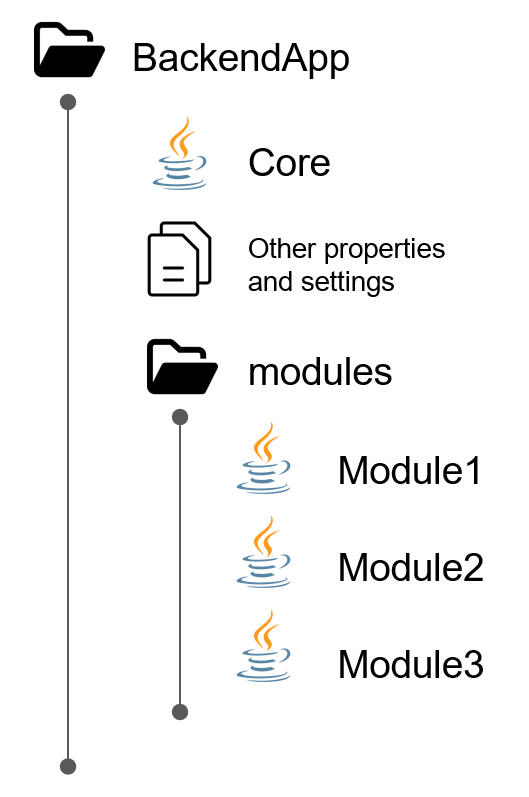
\includegraphics[scale=0.5]{images/plugin-folder-structure.png}
    \caption{Plugin architecture - Folder structure}
    \label{fig:figure1}
\end{figure}

\noindent In Figure \ref{fig:figure1}, the components labeled as core, module1, module2, and module3 represent packaged JARs. The core is responsible for detecting and loading the packaged Java sources from the modules folder. Typically, this task would require the use of a \textbf{ClassLoader}; however, Spring Boot simplifies this process for us. By utilizing Spring's loader properties \cite{springboot-loader-properties}, I can set the \hl{loader.path=file:modules/} property in the \textbf{loader.properties} file, located in the resources folder.
\\\\
The structure mentioned above presents various opportunities. For instance, in a distributed environment, if there's a need for a limited number of running instances but numerous lightweight microservices, instead of creating separate Spring Boot instances for each, they can all be appended to the same instance. Similarly, a small module responsible for logging or monitoring a specific microservice can be seamlessly integrated into the same instance. The environment can become even more dynamic if the loading and unloading of modules from the instance are controlled through commands given to the Spring Boot instance, such as REST API calls or periodic checks of a status flag inside each module, which can be externally updated.
\\\\
\noindent Ultimately, I concluded that continuing with this approach would introduce unnecessary complexity, especially since I didn't plan on adding numerous tightly coupled modules. Moreover, this strategy would necessitate the implementation of a plugin interface to specify the metadata of each service and an order loading mechanism to ensure that services dependent on others load after their dependencies are available.
\\\\
In the end, a simpler approach was chosen, but the above structure would still make an interesting choice in a more dynamic environment where there is a need for tightly coupled services that can be managed at runtime, using a plugin architecture.

\subsection{Final choice}


\noindent For this platform's use case, the final structure is organized as a \textbf{Maven project} with two Maven modules, thus adopting a \textbf{monolithic} approach. This approach simplifies the compilation and deployment of the modules within it. The parent pom defined in the main project allows for the specification of global parameters and configurations for shared dependencies. The modules themselves are implemented as \textbf{Spring Boot} projects, with one serving as a users microservice, functioning as an \textbf{authorization server}, and the other as a courses microservice (\textbf{resource server}), managing the official courses presented on the web platform. The authentication and authorization of resources is managed via \textbf{Spring Security}. Both Spring Boot applications are designed as \textbf{REST APIs}, following the \textbf{repository-service-controller pattern}.
\\\\
For the entire backend, I employ \textbf{Project Lombok} \cite{project-lombok}, a library that reduces code repetition and aids in writing cleaner code. An addition tool for boilerplate reduction is \textbf{MapStruct} \cite{mapstruct}, a library that generates mappers for classes automatically. For testing purposes, I utilize \textbf{JUnit} \cite{junit5} and \textbf{Mockito} \cite{baeldung-mockito}. Further details regarding library usage can be found in chapter \ref{Backend Explained}.

\newpage
\section{Frontend Framework}

Similar to the backend, my primary consideration for the frontend framework was focused on using a library with which I am familiar, specifically React.

\subsection{Initial attempts}

\noindent During my search for suitable frameworks, three names stood out to me: Vite (not a framework), Remix, and Next.js.

\subsubsection{Vite}

\noindent Vite, as described on its official website \cite{vite-guide}, is more of a frontend tool than a framework. It addresses common developer challenges by utilizing modern JavaScript features. With an integrated development server offering fast reloads and caching mechanisms, Vite significantly accelerates the development process. From what I have noticed, it is often chosen as an alternative to \textbf{Create React App}, boasting different bundling mechanics and notably faster performance. While Vite excels in client-side rendering, it lacks out-of-the-box support for server-side rendering, although this can be achieved through plugins.

\subsubsection{Remix}

\noindent After learning about Vite, I explored Remix, intrigued by its compatibility with Vite. According to their website \cite{remix-docs}, Remix is a framework built on top of React Router, serving as a compiler, server-side HTTP handler, server framework, and browser framework simultaneously. Although I see potential in Remix, particularly with its backing from Shopify, I faced challenges in finding necessary resources and specific use cases in their documentation. Consequently, I opted for a framework with a larger community, namely \textbf{Next.js}, as discussed in the final choice subsection.

\subsubsection{Modular frontend}

\noindent Regarding the frontend structure, I initially aimed for a modular approach, as I did for the backend. However, implementing this proved more challenging than anticipated. I considered utilizing monorepos as a solution, similar to the monolithic backend architecture. To manage this, I selected \textbf{Nx} \cite{nx-docs}, a build system designed for monorepos. Ultimately, navigating the complexities of Nx and its steep learning curve led me to abandon the idea of distinct microfrontends. Instead, I decided to only separate the modules structurally, as I considered it more suitable for my use case.

\subsection{Final choice}

\subsubsection{Why Next.js and not Remix}
\noindent Despite claims from one of Remix's co-founders that Remix matches, if not surpasses, Next.js in terms of speed \cite{remix-vs-next-according-to-remix}, I am inclined to favor Next.js for this web platform. While Remix may offer comparable performance, \textbf{Next.js} presents a larger ecosystem, providing abundant resources for specific use cases and ready-made solutions for common problems. Both Remix and Next.js are excellent solutions, but I personally found Next.js to be more accessible, both in terms of its features and documentation.
\\\\
\noindent Initially, I preferred Remix's routing approach, which allows you to specify all routes in the same file, whereas Next.js forces the usage of its file system route representation. This opinionated aspect initially concerned me, as I feared it would lead to a messy file hierarchy. However, in the end, I found this to be a beneficial standard, as it helps ensure that route segments remain manageable in length, by avoiding deep nesting. With the introduction of Next.js 13, a new App Router model was introduced, incorporating features such as Server Components, Streaming with Suspense, and Server Actions \cite{nextjs-app-router}. Although I initially used the Pages Router, I quickly migrated to the App Router to take advantage of its latest features. The transition was smooth, thanks to the documentation and support from the Discord community.

\subsubsection{Middleware}

\noindent One drawback of Next.js, in my view, is its tight integration of server and client aspects, which can occasionally lead to confusion about whether you are coding for the server side or client side of the application. Consequently, I have not considered using Next.js for the actual backend, preferring to keep the backend as a separate application. Therefore, the backend functionality of Next.js can be thought of as a \textbf{middleware} in the context of this web platform.

\subsubsection{Next.js Project}

\noindent The project was created using \hl{npx create-next-app@latest} \cite{nextjs-installation}, with \textbf{TypeScript}, \textbf{ESLint}, \textbf{Tailwind CSS} and \textbf{App Router} selected. On top of this, I also use \textbf{Prettier} \cite{prettier}, an opinionated code formatter in the Next.js project.
\\\\
\noindent \textbf{TypeScript} enhances code maintainability by introducing static typing to JavaScript variables. This allows the compiler and linter to detect potential issues such as incorrect type conversions or accessing undefined fields before they cause problems in production. Additionally, TypeScript enables text editors to provide context-aware suggestions based on variable types, leading to a more efficient development process. Since all TypeScript code is eventually compiled into JavaScript during the build process, there are no compatibility issues to worry about.
\\\\
\noindent \textbf{ESLint} is employed to enforce coding standards and maintain overall code quality. It identifies syntax errors, potential bugs, and problematic patterns, helping developers adhere to best practices and ensure consistency across the codebase.
\\\\
\noindent \textbf{Tailwind CSS} simplifies the project by eliminating the need for separate CSS files. Instead, styles are applied using predefined class names, reducing the overhead of managing custom class names and allowing for dynamic customization through class variants. Furthermore, Tailwind automatically removes unused styles during the bundling process, optimizing the CSS output.

\section{Frontend Optimization}

NextJS by itself already provides a lot of optimizations, such as automatic code splitting, image optimization, and server-side rendering. However, there are still some optimizations that can be done to improve the performance of the web platform.

\subsection{SWR}

\noindent SWR (stale-while-revalidate) is a strategy for caching data in the frontend, which is used for data that changes frequently. By using SWR, the web platform can display the latest data while also updating the cache in the background. This approach ensures that the user always has access to the most up-to-date information without sacrificing performance.
\\\\
\noindent Based on the previous invalidation strategy, a library with the same name, \textbf{SWR} \cite{swr}, is used. SWR is a React Hooks library for data fetching that provides out of the box ways to cache data, revalidate it, and handle errors. It is used on the client side to fetch data from the backend.

\section{Databases}

\subsection{H2 Database}

\noindent H2 \cite{h2} is a lightweight relational database management system, written in Java, which when used with Spring Boot, can be a fast solution for development and testing, as it acts as an in memory database. Since it supports SQL syntax, I am using it as a dummy database, executing the same queries I would for PostgreSQL, but without having to reset the database on each test instance.

\subsection{PostgreSQL}

\noindent PostgreSQL \cite{postgresql}, a relational database management system, is used for managing user data in this web platform. It handles critical information like personal details and refresh tokens. PostgreSQL was a top candidate when choosing, due to my prior experience with it, as well as its adherence to ACID principles, ensuring data integrity and reliability even under heavy user loads. Additionally, its open-source nature and permissive licensing model made it an attractive choice, especially compared to proprietary options like Oracle.
\\\\
\noindent The decision to use a relational database instead of a non-relational one was deliberate, considering the structured nature of the data and the need for a robust architecture to support complex relationships and transactions.

\subsection{MongoDB}

\noindent MongoDB \cite{mongodb} stands out as one of the preferred options for non-relational databases, especially in scenarios where data lacks a structured format. In the context of this web platform, a non-relational database was essential for managing course information due to its unstructured nature. Each course is represented as a JSON object with varying levels of depth, featuring a recursive structure of components that can nest within each other. MongoDB's capability to conduct full-text searches via specialized text indexes has proven to be a valuable asset. While it may not offer the complexity of search indexing seen in Elasticsearch, MongoDB's functionality proved sufficient for conducting course searches within the web application.

\subsection{Connecting to database}

\noindent Connection to the databases mentioned above is done through Spring Boot, especially through Spring Data \cite{spring-data}. For PostgreSQL and H2, I use Spring Data JPA with Hibernate, and also HikariCP \cite{hikaricp} for connection pooling. For MongoDB, Spring Data MongoDB is used.
\\\\
\noindent \textbf{JPA}, or Java Persistence API, serves as an interface defining standards for database manipulation, along with providing a native object-oriented query language known as JPQL.
\\\\
\noindent \textbf{Hibernate} is an implementation of the JPA guidelines, providing its own object-oriented query language as well, HQL.
\\\\
\noindent As Spring Data JPA is an integration for JPA, \textbf{Spring Data MongoDB} is an integration for MongoDB, offering a template helper class, data repositories, multiple document transactions and other useful features. 

\section{Deployment}

The web platform was designed with two profiles in mind: \textbf{development} and \textbf{production}. The development profile is intended for local testing and debugging, while the production profile is meant for deployment on a server. The deployment process is facilitated by \textbf{Docker} \cite{docker} and \textbf{Docker-Compose} \cite{docker-compose}, which allow for the creation of containers for the backend, frontend, and database. These containers are then orchestrated using Docker-Compose, ensuring that the web platform runs smoothly in a production environment.

\subsection{Running and Compiling}

\subsubsection{Backend}

\noindent For development purposes, the backend modules are run inside IntelliJ IDEA by executing the main class of each module. To run the modules successfully, some environment variables must be set. For this, a \textbf{.env} file is created in the root of each module, containing the necessary variables. A JetBrains plugin called \textbf{EnvFile} is used to load the environment variables from the .env file into the IDE. By default, the project is configured in Maven to use the \textbf{dev profile}.
\\\\
\noindent If the \textbf{prod profile} is selected, the modules can also be run using the above method, simulating a production environment. For example, it might be more accessible to test that the users module's production database (PostgreSQL) is running as expected, and there are no compatibility issues with the development database (H2), by running it directly in the IDE instead of compiling and testing outside it.
\\\\
\noindent After obtaining satisfying results with the previous method, the modules are compiled using Maven by running \hl{mvn clean package -P prod}, which generates a JAR file for each module using the \textbf{prod profile}. The JAR files are then run using the \hl{java -jar} command, with the necessary environment variables set.

\subsubsection{Frontend}

\noindent The frontend is run using the \hl{npm run dev} command, which starts the development server. The development server is accessible at \textbf{http://localhost:3000}. The frontend can also be run in production mode by running the \hl{npm run build} command, which compiles the NextJS project, followed by the \hl{npm run start} command. The production server is accessible at the same URL.
\\\\
\noindent The frontend also relies on environment variables, which are set in a \textbf{.env.local} file in the root of the frontend project and are automatically loaded by NextJS. Three files are used for environment variables: \textbf{.env.local} for local development, \textbf{.env.development} for development, and \textbf{.env.production} for production. Variables from the .env.local file have a higher priority, while the other two files are conditionally loaded based on the environment.
\\\\
\noindent \textbf{Attention!} NextJS will try to optimize many aspects of the application, but some of these optimizations might affect the behavior of the web platform. For example, NextJS caches all fetch requests by default, but this caching is not visible in development mode. If not careful, this might lead to unexpected results when testing the application, such as never-changing data, even if the backend has been updated.

\subsection{Docker}

\noindent Docker is a platform that simplifies the deployment process by packaging applications and their dependencies into containers. Containers are portable and isolated, ensuring that the contents run the same way in any environment. Docker also provides a centralized repository for storing and sharing container images, known as Docker Hub.
\\\\
\noindent To assist with the deployment process, a \textbf{Dockerfile} was created for each backend module, containing the necessary instructions for building the image. The Dockerfile for the backend modules is based on the \textbf{eclipse-temurin:17-jre-alpine} image and copies the compiled module JAR file into the image.
\\\\
\noindent The frontend also has a Dockerfile, based on the \textbf{node:18-alpine} image, with two stages: one for building the project and one for running it. The compiled project is copied into the second phase, which is then used to run the project. The frontend Dockerfile also contains the necessary instructions for installing the required dependencies and setting the environment variables.
\newpage
\noindent Although containers for the backend modules and frontend are created only for deployment, databases are needed in both development and production environments. For this reason, local containers were created and used for them. To visualize the data inside them, \textbf{pgAdmin} was used for PostgreSQL, and \textbf{mongo-express} for MongoDB.

\subsection{Docker-Compose}

\noindent Docker is a powerful tool for managing containers, but it can be challenging to orchestrate multiple containers manually, especially as the number of services increases.
\\\\
\noindent Docker-Compose is a tool for defining and running multi-container Docker applications. It simplifies the process of managing multiple containers by allowing users to define the services, networks, and volumes in a single file. The Docker-Compose file for the web platform contains the services for the backend, frontend, and database, as well as the necessary environment variables.
\\\\
\noindent The Docker-Compose file is used to build the images for the backend modules and frontend, as well as to create the containers for the database services. The containers are then started using the \hl{docker-compose up --build} command, which builds images and runs the services defined in the file. The web platform is accessible at \textbf{http://localhost:3000}.
\\\\
\noindent For communication between Docker services, a network is created by Docker-Compose, allowing the services to communicate with each other. Each service is accessible to the others by using the service name as the hostname, as defined in the Docker-Compose file.
\\\\
\noindent Tweaks can be made to the Docker-Compose file to modify the behavior of the services on a production server. For example, exposing specific ports, setting environment variables, or defining volumes for persistent data storage.

\subsection{Extending}

\noindent As the application grows, a CI/CD pipeline such as \textbf{Jenkins} can be implemented to automate the deployment process. This pipeline can be used to build, test, and deploy the application to a server, ensuring that the latest changes are always available to users. \textbf{Kubernetes} can also be used to manage the containers in a production environment, ensuring that the application is always available and scalable.
\chapter{Backend Explained} \label{Backend Explained}

In this chapter I will document the contents of the backend project and challenges met along the development process.

\section{Project Configuration}

\subsection{Parent Project}

\noindent The backend main project is a multi-module Maven project. 
In a multi-module Maven project, the parent POM (Project Object Model) serves as the primary configuration file that defines common settings, dependencies, and plugins for all the modules within the project. It helps to centralize and manage configurations that are shared across multiple modules, promoting consistency and reducing redundancy. Additionally, the parent POM can define build profiles, repositories, and other project-wide settings that are inherited by all child modules.
\\\\
\noindent In the \textbf{pom.xml} from \hl{/backend/pom.xml} (Figure \ref{fig:figure2}), essential metadata settings are defined, including groupId, artifactId, version, modules, and packaging. Additionally, a parent is specified, namely \hl{spring-boot-starter-parent} from org.springframework.boot, which provides default configurations and dependencies for Spring Boot applications. Right after, global variables are utilized to specify the Java version (17), set the project encoding as UTF-8, and define other reusable values, such as library versions. Following this, \textbf{two profiles}, "dev" and "prod", are declared to facilitate switching between running modes. These profiles determine the file configurations used in the Spring Boot applications. Next, \textbf{dependencies} and \textbf{dependencyManagement} settings are specified. The \hl{spring-boot-starter-web} from org.springframework.boot is added as a dependency to all modules, pulling in web development-related dependencies like an embedded Tomcat server and data binding. DependencyManagement, a setting specific to the parent pom.xml, provides general configurations for potential dependencies without directly including them. It primarily serves to globally specify library versions, eliminating the need to specify versions in each file when imported in modules. Similarly, within the \textbf{build} setting, \textbf{plugins} and \textbf{pluginManagement} are utilized. The \hl{maven-compiler-plugin} is imported in all modules for packaging applications into JARs. In pluginManagement, configuration settings for the mapping library \textbf{MapStruct} are specified, and \hl{spring-boot-maven-plugin} is instructed to exclude Project Lombok's code. These configurations can be overridden in child modules if necessary.

\begin{figure}[h]
    \centering
    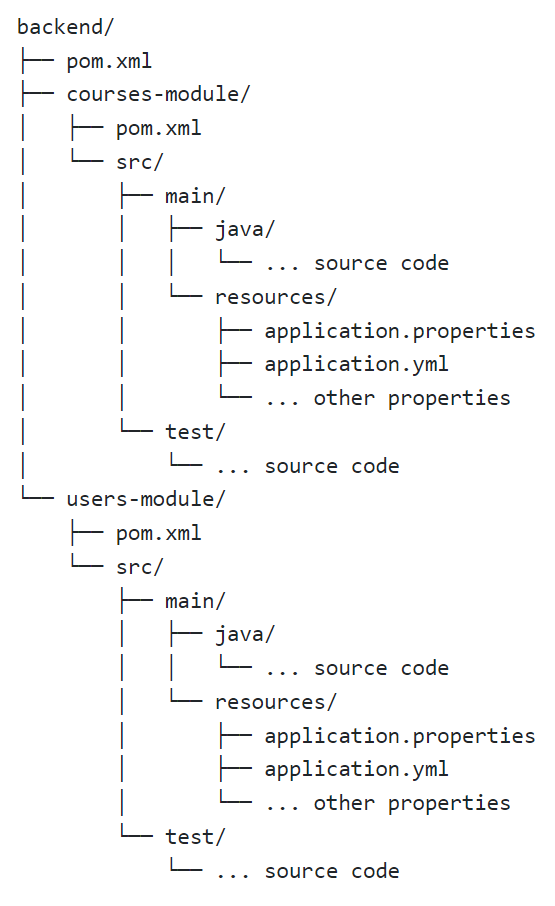
\includegraphics[scale=0.7]{images/backend-folder-structure.png}
    \caption{Backend - Folder structure}
    \label{fig:figure2}
\end{figure}

\subsection{Users Module Project} \label{Users Module Project}

\noindent In the \textbf{pom.xml} from \hl{/backend/users-module/pom.xml} (Figure \ref{fig:figure2}), alongside standard metadata, the dependencies utilized in this module are declared. These dependencies include \textbf{mapstruct}, \textbf{mapstruct-processor}, \textbf{lombok}, \textbf{spring-boot-starter-data-jpa}, \textbf{hibernate-core}, \textbf{hibernate-hikaricp}, \textbf{postgresql}, \textbf{spring-boot-starter-test}, \textbf{junit-jupiter-api}, \textbf{h2}, \textbf{jjwt-api}, \textbf{jjwt-impl}, \textbf{jjwt-jackson}, and \textbf{caffeine}. Further details about their usage will be provided in subsequent sections.
\\\\\newpage
\noindent In the \textbf{resources folder} from \hl{/backend/users-module/src/main/resources} (Figure \ref{fig:figure2}) are located configuration and property files for Spring Boot.
\\\\
\noindent A \textbf{banner.txt} file that is displayed right in the beginning of the application. It contains written in big text the name of the module, as well as the module's version and spring boot's version. This information can be useful for monitoring and letting you know if you are running with outdated software.
\\\\
\noindent When it comes to application settings, Spring Boot automatically recognizes two types of files: \textbf{application.yml} and \textbf{application.properties}. The distinction lies in their usage, as application.properties supports only string values, while application.yml is better suited for handling complex values and nested properties. In the users module, both types of files are used. This approach allows for a separation between common and generic settings in application.yml, while custom properties are managed in application.properties.
\\\\
\noindent In the configuration from inside \textbf{application.yml}, the \textbf{server.port} property specifies the port used to start the Embedded Tomcat Server. It's crucial to assign a unique port to avoid conflicts with other applications. The \textbf{spring.profiles.active} property determines the active profiles for the application, obtained through the \textbf{@activatedProperties@} placeholder, replaced by Maven based on the \textbf{<activatedProperties>} tag.
\\\\
\noindent The section for configuring the HikariCP \cite{hikaricp} connection pool includes properties such as \textbf{connection-timeout}, \textbf{idle-timeout}, \textbf{max-lifetime}, \textbf{minimum-idle}, \textbf{maximum-pool-size}, and \textbf{pool-name}. These properties define parameters like maximum wait time for a connection, maximum idle time, maximum lifetime of a connection, minimum number of idle connections, maximum pool size, and the pool name, respectively.
\\\\
\noindent The properties \textbf{ddl-auto} and \textbf{show-sql} relate to Hibernate and JPA. ddl-auto specifies how Hibernate handles database schema updates based on entity mappings, set here to "update" to allow for automatic schema updates based on their corresponding Java entity. show-sql controls whether queries executed by Hibernate are logged, aiding in debugging database operations and helping with performance, allowing you to see if manual query optimization is required.
\\\\
\noindent Finally, \textbf{server.error.include-message} determines whether error messages are included in error responses sent by the server. In this case, error messages are included, aiding in debugging and error handling for the REST API backend. By default, these messages are hidden to prevent leakage of private code logic information, but that is handled via custom error processors in this web platform.
\\\\
\noindent Based on selected profile, Spring Boot can use conditional files. For example, for an active profile x and an inactive profile y, \mbox{\textbf{application-x.properties}} will be loaded but \mbox{\textbf{application-y.properties}} will not.
\\\\
\noindent In the \textbf{application-dev.properties} file of the users module, several settings are configured to manage database connectivity, H2 console access, JPA behavior, data seeding, and logging levels. The \textbf{spring.datasource.url} setting specifies the URL used to connect to the database, with the example provided connecting to an H2 in-memory database named DesignOOP-UsersDB. Credentials for database authentication are defined with \textbf{spring.datasource.username} and \textbf{spring.datasource.password}, set to sa and an empty string, respectively, for running an instance of the module in development mode. The JDBC driver class name is specified with \textbf{spring.datasource.driver-class-name}, set to org.h2.Driver for the H2 database. The \textbf{spring.h2.console.enabled} setting determines whether the H2 console is enabled, allowing browser-based interaction with the database when set to true. Additionally, the Hibernate dialect for JPA is configured with spring.jpa.database-platform, set to org.hibernate.dialect.H2Dialect for compatibility with H2. Data seeding, the process of populating the database with initial data, is controlled by \textbf{app.data.seeding.enabled}, set to true to enable seeding. This feature is needed for testing purposes, as H2 is used as an in-memory database, that resets its content on each restart. Finally, logging levels for specific packages or classes are configured with logging.level, with debug-level logging enabled for Spring MVC method invocation (\textbf{org.springframework.web.servlet.mvc.method.annotation}) and Spring Security-related classes (\textbf{org.springframework.security}).
\\\\
\noindent In the \textbf{application-prod.properties} file of the users module, database connectivity settings are configured to connect to a PostgreSQL database. The \textbf{datasource.url}, \textbf{datasource.username}, and \textbf{datasource.password} settings specify the JDBC URL, username, and password for accessing the database, respectively. These values are placeholders (\$\{POSTGRES\_URL\}, \$\{POSTGRES\_USERNAME\}, \$\{POSTGRES\_PASSWORD\}) that are replaced with actual values stored in environment variables or property files. The database type is set to PostgreSQL via \textbf{jpa.database}, and the JDBC driver class name is specified with \textbf{datasource.driver-class-name}, set to org.postgresql.Driver for PostgreSQL databases. Additional Hibernate properties are configured with \textbf{jpa.properties}, including \textbf{hibernate.format\_sql} set to true to format SQL queries for readability, and hibernate.dialect set to \textbf{PostgreSQLDialect} to specify the dialect for PostgreSQL databases.
\\\\
\noindent The \textbf{application.properties} file contains custom settings regarding JWT settings.

\subsection{Courses Module Project}

\noindent In the \textbf{pom.xml} from \hl{/backend/courses-module/pom.xml} (Figure \ref{fig:figure2}) are declared the dependencies for the course module. They include \textbf{mapstruct}, \textbf{mapstruct-processor}, \textbf{spring-boot-starter-data-mongodb}, \textbf{spring-boot-starter-security}, \textbf{spring-boot-starter-oauth2-resource-server}, \textbf{spring-security-oauth2}, \textbf{lombok}. Further details about their usage will appear in subsequent sections.
\\\\
\noindent Configuration and property files for Spring Boot are located in the \textbf{resources folder} from \hl{/backend/courses-module/src/main/resources} (Figure \ref{fig:figure2}). The purpose of the files present in this folder (\textbf{banner.txt}, \textbf{application.yml}, \textbf{application.properties}, \textbf{application-[profile].properties}) is already described in the beginning of the \ref{Users Module Project} subsection.
\\\\
\noindent In the configuration provided, the \textbf{server.port} property specifies the port for the Embedded Tomcat Server, ensuring it operates on a unique port to avoid conflicts with other applications. The \textbf{spring.profiles.active} property determines the active profiles for the application, dynamically assigned based on Maven's \textbf{<activatedProperties>} tag, allowing for flexible configuration.
\\\\
\noindent The section for configuring the MongoDB database includes properties such as \textbf{auto-index-creation}, \textbf{authentication-database}, \textbf{username}, \textbf{password}, \textbf{database}, \textbf{host}, and \textbf{port}. These properties define parameters such as auto-index creation, authentication details, database credentials, and connection details, ensuring seamless integration with the MongoDB database. Some of the previously mentioned fields use placeholders, that will be replaced by environmental variables (\$\{mongodb\_username\}, \$\{mongodb\_password\}, \$\{mongodb\_database\}, \$\{mongodb\_host\}, \$\{mongodb\_port\}).
\\\\
\noindent The \textbf{server.error.include-message} property determines whether error messages are included in error responses sent by the server. Enabling this property aids in debugging and error handling for the REST API backend. By default, these messages are hidden to prevent leakage of private code logic information, but custom error processors handle them within this web platform.
\\\\
\noindent When the development profile is active, extra debugging information is enabled via the \textbf{logging.level.org.springframework.web.servlet.mvc.method.annotation} and the
\textbf{logging.level.org.springframework.security} properties, which are set to "DEBUG" inside the \textbf{applications-dev.properties} file.

\section{Folder structure of a module}

To ensure code maintainability, all modules in this web platform representing Spring Boot applications follow the folder structure shown in Figure \ref{fig:figure3}.

\begin{figure}[h]
    \centering
    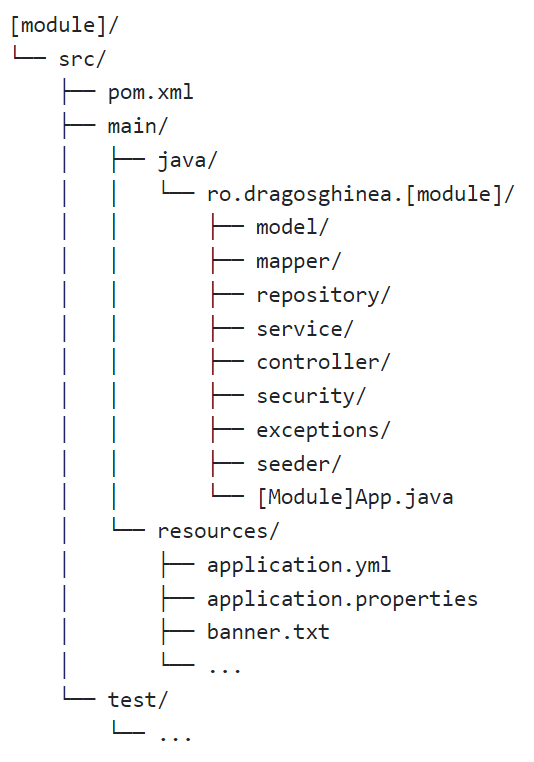
\includegraphics[scale=0.7]{images/module-folder-structure.png}
    \caption{Module - Folder structure}
    \label{fig:figure3}
\end{figure}

\noindent This folder structure is a template for the modules, but if required, more packages could be created besides the ones specified in \hl{ro.dragosghinea.[module]}. In fact, from the ones mentioned in Figure \ref{fig:figure3}, only \textbf{model}, \textbf{repository}, \textbf{service}, \textbf{controller} are crucial, as they are the base of the repository-controller-service pattern that I try to enforce in Spring Boot modules. More details regarding each package present in the main folder of the module are described in the following sections.

\section{Repositories}

In the repository-service-controller pattern, the role of the repository classes is to communicate with the database, executing transactions. As a separation of concerns and structured hierarchy, repositories are supposed to only be accessed by the services. For repositories, important are the \textbf{repository} and \textbf{model} packages from Figure \ref{fig:figure3}.
\\\\
\noindent Inside \textbf{repository} are defined repository interfaces, that contain methods for interacting with the database. These interfaces have automatic implementations by Spring Data, which are influenced by method definitions and, if necessary, custom queries specified using the \textbf{@Query} annotation. Notably, complex queries can be automatically generated based on method names. For instance, the method signature \verb|List<Person>| \verb|findDistinctPeopleByLastnameOrFirstname(String lastname, String firstname);| produces a query that precisely fulfills its name's intent. For further insights into this behavior, refer to \cite{spring-data-repositories}. Additionally, Spring Data can accommodate different return types, such as returning \textbf{null} for a find method with a return type of \textbf{Entity}, or an \textbf{Optional<Entity>} returning an empty value.
\\\\
\noindent In the \textbf{model} package, you'll find classes designated as entities, which are utilized by Spring Data to interact with the database. Additionally, this package contains special objects known as data transfer objects (DTOs), which facilitate communication with higher layers such as services and controllers. Data transfer objects serve a crucial role in decoupling, as their usage detaches information from the database. Direct manipulation of entities can inadvertently trigger unwanted database updates, making DTOs a preferred choice for communication between layers or anywhere outside the database interaction domain.

\subsection{Users Module}

\subsubsection{Model}

\noindent The users module uses Spring Data JPA as the primary interface, implemented via Hibernate. The entities of the module are created via \textbf{@Entity} and \textbf{@Table} annotations. The @Entity annotation marks the class as a JPA entity. The @Table annotation allows customization of the entity, allowing the addition of foreign keys and changing the name of the table used for the entity (by default, the class name is also the table name).

\begin{figure}[h]
    \centering
    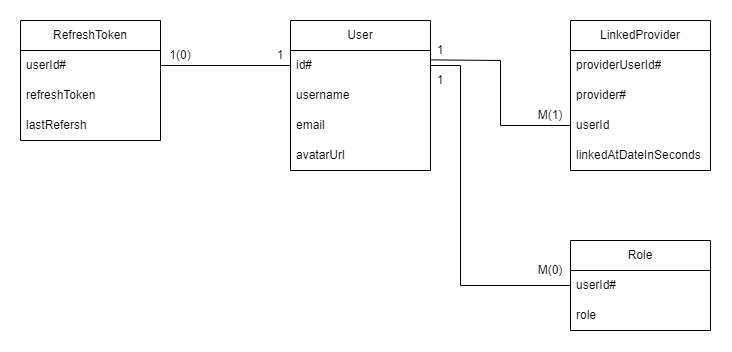
\includegraphics[scale=0.6]{images/users-schema.png}
    \caption{Users Database Schema}
    \label{fig:figure4}
\end{figure}

\newpage
\noindent In the users module, there are corresponding classes for the entities represented in Figure \ref{fig:figure4}. Classes annotated with \textbf{@Entity} are RefreshToken, User, and LinkedProvider. The Role entity is not an actual class, as the annotation \textbf{@ElementCollection} is used inside the User entity. This annotation automatically takes an iterable collection and maps it to a separate table.
\\\\
The \textbf{@Table} annotation is used for two purposes in this module. Firstly, to rename the User entity to "User\_", as the name without an underscore seems to be reserved by the database's internal mechanics. This is done via \textbf{@Table(name="USER\_")}. The second purpose is declaring unique key constraints, done via the {@Table(uniqueConstraints = {...}} in the LinkedProvider entity. Besides the composite primary key, the LinkedProvider should have the unique composite key \textbf{(provider, userId)}, ensuring a user doesn't have two external providers of the same type linked. Code wise, the unique constraint is defined via \textbf{@UniqueConstraint(name="OneProviderPerUser", columnNames = \{"user\_id", "provider"\})}.
\\\\
\noindent In the model classes, entity relationships are defined using fields with special annotations. The relationship between the LinkedProvider and User entities is established through two fields, although only one is necessary for the relationship to be recognized. In the LinkedProvider class, the \textbf{\textit{private User user;}} field is annotated with \textbf{@ManyToOne}. This annotation includes a parameter (fetch=FetchType.LAZY), instructing Hibernate to retrieve this field from the database only when it's accessed via a call. Similarly, the User class denotes the relationship with the \textbf{@OneToMany} annotation and the \textbf{\textit{List<LinkedProvider> linkedProviders;}} field. The \textbf{cascade = CascadeType.ALL} parameter ensures that all linked providers are deleted if the corresponding user is deleted, allowing for cascading events. Incorporating both the userId and user field within the LinkedProvider presented some challenges, which were addressed by adding two annotations. The userId field is annotated with @Column(user\_id), while the user field uses @JoinColumn(name = "user\_id", referencedColumnName = "id", insertable = false, updatable = false). The @JoinColumn annotation enables the entity to exist without automatically persisting modifications to the database made through the user field. A similar relationship is established between the User and RefreshToken entities.
\\\\
\noindent In addition to the entities, corresponding DTOs are created to facilitate communication in upper layers such as services and controllers. Alongside these entity-specific DTOs, there are also additional DTOs that don't directly correspond to specific entities but contain information utilized for certain requests.

\subsubsection{Repository}

\noindent In the users module, repositories are interfaces that extend the \textbf{JpaRepository<\\EntityClass, EntityIdClass>} type. This JpaRepository, a part of Spring Data, inherits functionality from CrudRepository, which handles CRUD operations like findById, save, and deleteById, as well as from PagingAndSortingRepository, which adds methods for pagination and sorting. With repositories defined for nearly all entities shown in Figure \ref{fig:figure4}, automatic and custom-generated queries are utilized. An automatic query example is \textit{LinkedProvider findByProviderUserIdAndProvider(String providerUserId, ProviderType provider)}, which performs the action described by its method name. Custom queries are also employed in the users module, such as the need to eagerly load a lazy field without making two trips to the database, as demonstrated by the annotation \textit{@Query("SELECT rt FROM RefreshToken rt JOIN FETCH rt.user WHERE rt.userId = :userId")}.

\subsection{Courses Module}

\subsubsection{Model}

\noindent The courses module uses Spring Data MongoDB, where entities are annotated with \textbf{@Document}. MongoDB was chosen for its suitability to handle dynamic elements like courses, which may evolve over time without a fixed design. For instance, if additional metadata needs to be added to course objects in the future, MongoDB seamlessly accommodates these changes without requiring database refactorings, as its document-based structure automatically adapts to new fields. The recursive nature of the component tree in courses would have posed challenges with a relational database, given its lack of structured definition. Since courses are manipulated as JSONs on the frontend and no complex queries benefiting from relational databases are anticipated on the server side, MongoDB emerged as the optimal choice, offering storage in BSON format closely aligned with JSON.
\\\\
\noindent The courses module's most complex operation is the \textbf{full-text search feature}, aimed at retrieving relevant courses based on user input. Initially, specialized database systems like Elasticsearch were considered for their scalability and indexing capabilities. However, configuring support for both MongoDB and Elasticsearch proved challenging and excessive for the current use case. While Elasticsearch remains a viable option for future scalability needs, the chosen approach for the current platform is to utilize MongoDB's built-in text search feature.
\\\\
\noindent To enable this feature, the Course entity defines multiple text indexes using \textbf{@TextIndexed} with varying weights, which are later merged into a single full-text search index applied to the database. It's essential to ensure that \textbf{auto-index-creation} is set to true in Spring Boot's properties to facilitate index creation.
\\\\
\noindent The \textbf{full-text search} functionality matches against multiple properties with different weights to calculate a relevancy score. These properties, ranked in order of importance from highest to lowest, include title, tags, subtitle, description, and components content. For specifying the weights for each property, the weight parameter is utilized in the @TextIndexed annotation. The text score is returned inside the entity via a float field, annotated with @TextScore.

\subsubsection{Repository}

\noindent In the courses repository, the Spring Data \textbf{MongoRepository<EntityClass, EntityIdClass>} interface is extended along with a custom CourseSearchRepository interface. Similar to JpaRepository used in the users module, MongoRepository provides common CRUD and pagination methods.
\\\\
\noindent The custom CourseSearchRepository interface exposes a new method: \textit{Page<Course> search(String query, int pageNumber, int pageSize, boolean fetchWithoutComponents)}. This method conditionally excludes the \textbf{components} field from the returned values based on the fetchWithoutComponents parameter. This optimization reduces payload size since only metadata, not content, is essential for presenting search results to users.
\\\\
\noindent The CourseSearchRepository interface is implemented through a custom implementation, \textbf{CourseSearchRepositoryImpl}, which utilizes MongoTemplate to execute the search query. In this implementation, the query string is matched as a case-insensitive phrase with ignored diacritics. The resulting List, wrapped in a Page format, is sorted by the text score. Spring automatically detects and uses the custom implementation of CourseSearchRepository. The custom implementation was done with the help of the following online resource: \cite{mongodb-custom-repositories}.

\section{Services}

Services, responsible for executing algorithms, manipulating data, and interfacing with repositories, constitute the business logic layer in the web platform's modules. They are mainly called by controllers or other services, while they, in turn, call repositories. Ideally, they should all reside within the \textbf{service} package, as indicated in Figure \ref{fig:figure3}, with the exception of security-related services, which are placed separately in the security package.
\\\\
\noindent Mappers, essential for converting objects between different types, are predominantly utilized in the backend for mapping DTOs to entities and vice versa. The web platform uses \textbf{MapStruct} to automate the generation of mappers. This library identifies interfaces annotated with \textbf{@Mapper} and compiles implementations during build time. However, a challenge arises due to caching issues, where changes to mapped classes may not trigger the generation of new implementations. Consequently, runtime errors may occur during mapping attempts. To avoid this issue, it's advisable to perform a Maven clean operation before compiling, or at least upon encountering mapper-related errors.

\subsection{Users Module}

\noindent In the users module, the primary focus lies on authentication. Several services handle authentication against various linked providers like Discord or GitHub. Additionally, there's a general authentication service responsible for invoking the appropriate service based on the input type. Apart from these, there are two services dedicated to CRUD operations: one for user CRUD and another for refresh tokens CRUD. Further details on refresh tokens can be found in the security section.
\\\\
\noindent Within this module, service methods declare their return type and parameters using DTOs, while internally operating with entities. Consequently, each service requires both a repository instance and a mapper instance. To address this, a compositional approach is adopted. Fields for the necessary instances are defined within the services and initialized via a parameterized constructor. Lombok facilitates this process with its \textbf{@RequiredArgsConstructor} annotation, which automatically generates a constructor with parameters for all final fields within the annotated class. Spring Boot handles the instantiation of these services through \textbf{dependency injection}. By recognizing the dependencies of a constructor, Spring Boot constructs and retains instances of those dependencies, injecting them when creating instances of the parameterized service.

\subsection{Courses Module}

\noindent In the courses module, the primary focus revolves around resource management. Consequently, the service within this module is responsible for handling CRUD operations related to courses. Unlike JPA, the MongoDB integration of Spring Data does not automatically persist changes and is not as tightly coupled to the database session. Therefore, the decision was made not to create a DTO for the course object. However, in the context of DTOs, a class was created specifically to facilitate communication of page data to the controller. This class, named PageDto, is essentially a mapping of Spring's Page class, but with select fields renamed and additional fields added as needed.

\section{Controllers}

Controllers serve as the entry point for a REST API, exposing routes that can be accessed via HTTP requests. They orchestrate the business logic defined in services, maintaining a separation of concerns by communicating only with services and not directly with repositories. In this web platform, controller classes are located in the \textbf{controller} package (Figure \ref{fig:figure3}), identified by the \textbf{@RestController} annotation.
\\\\
\noindent Routes are defined using annotations, such as \textbf{@RequestMapping}, which sets the base route for all methods within the class, and method-specific annotations like \textbf{@GetMapping}, \textbf{@PostMapping}, \textbf{@DeleteMapping}, and \textbf{@PutMapping} to define the HTTP methods for individual routes. These annotations can also have a value parameter to extend the route specified by the controller class.
\\\\
\noindent Data validation is automatically handled by Spring Boot, rejecting requests with parameters that don't match the method's object parameters. Additional validation, like password length or email format, can be implemented separately. Annotations like \textbf{@RequestHeader}, \textbf{@RequestParam}, \textbf{@PathVariable}, and \textbf{@RequestBody} are used to extract data from different parts of the request, such as headers, query parameters, dynamic path segments, and the request body, respectively. There are other specialized annotations available for specific request elements as well.
\\\\
\noindent For \textbf{exception handling}, three approaches are employed, inspired by \cite{baeldung-spring-exceptions}. \textbf{The first approach} involves handling exceptions at the controller layer. If an error occurs within a controller method, a \textbf{ResponseStatusException} is thrown to indicate the specific HTTP status code and error message. \textbf{The second approach} utilizes a global controller exception handler defined using \textbf{@ControllerAdvice}. This class can intercept and handle errors thrown within controllers, allowing for centralized exception handling and customization of the response. \textbf{The third approach} involves annotating exceptions thrown by services with \textbf{@ResponseStatus}. This annotation specifies the HTTP status code to be returned when the exception is encountered, allowing the default error resolver to handle it appropriately.

\begin{lstlisting}[style=json, frame=single, caption={error response format}, label={lst:listing1}]
{
    "timestamp": date string,
    "status": HttpStatusCode,
    "error": HttpStatusError,
    "message": error string,
    "path": route string
}
\end{lstlisting}

\noindent In listing \ref{lst:listing1}, the error format follows a standard commonly used in Spring Boot applications. It includes several key fields: \textbf{timestamp} indicates the exact time when the error occurred, formatted as an ISO 8601 string (YYYY-MM-DDTHH:MM:SS.sss±hh:mm); \textbf{status} represents the HTTP status code of the response to the request; \textbf{error} denotes the associated error category corresponding to the error status (e.g., "Not found" for error status 404); \textbf{message} provides a human-readable error message; \textbf{path} specifies the route at which the error was thrown.

\subsection{Users Module}

In this subsection, the entry points of the users module are explained, resembling a REST API documentation. This module consists of two controllers with distinct purposes. One controller manages authentication and token generation, handling routes starting with \textbf{/v1/auth}, while the other allows user profile customization and manages routes starting with \textbf{/v1/users}.
\\\\
\noindent The \textcolor{olive}{GET} \textbf{/v1/users/me} route fetches the user details for the currently logged-in user. An unauthorized request response is sent if this route is accessed without an authenticated user.
\\\\
\noindent The \textcolor{cyan}{PATCH} \textbf{/v1/users/me} route updates user details. It receives a body with the fields of the user that need an update. It can be a single field or multiple.
\\\\
\noindent The \textcolor{orange}{POST} \textbf{/v1/auth/login} route handles user login, expecting a clientRegistrationId and an accessToken in the request body. The clientRegistrationId represents the OAuth2 provider (e.g., Discord or GitHub), while the accessToken is a valid OAuth2 access token. Upon validation, user information is extracted and a new access token with a refresh token is returned.
\\\\
\noindent The \textcolor{orange}{POST} \textbf{/v1/auth/logout} route simply logs out the currently authenticated user that executes the request.
\\\\
\noindent The \textcolor{orange}{POST} \textbf{/v1/auth/refresh} route generates a new access token based on a refresh token. The refresh token can be passed as a header (\textbf{refresh-token}) or as a parameter in the request body (\textbf{refresh\_token}). To optimize performance, a cache using the \textbf{Caffeine} library stores recently generated tokens for 3 seconds, preventing excessive token regeneration. If a cache value is returned, the response body will signal it via a message field.
\\\\
\noindent The \textcolor{orange}{POST} \textbf{/v1/auth/validate-token} route validates backend access tokens (not OAuth2 tokens generated by Discord or GitHub), returning a response status code of 200 for valid tokens and 401 for invalid ones.

\subsection{Courses Module}

In this subsection, the entry points of the courses module are explained, resembling a REST API documentation.
\\\\
\noindent The \textcolor{olive}{\textbf{GET}} \textbf{/v1/courses} route retrieves courses and accepts optional query parameters: \textbf{pageNumber} (default: 0), \textbf{pageSize} (default: 20), and \textbf{search} for filtering courses based on a phrase. Additionally, the custom request header \textbf{X-Fetch-Without-Components} can be provided to optimize payload by excluding course components when unnecessary.
\\\\
\noindent The \textcolor{orange}{\textbf{POST}} \textbf{/v1/courses} route creates a new course. It expects a request body containing all course fields except the ID, which is optional and auto-generated if absent. The newly created course is returned, containing the generated ID if one was not given.
\\\\
\noindent The \textcolor{blue}{\textbf{PUT}} \textbf{/v1/courses/\{courseId\}} route updates a course identified by \{courseId\}. It receives the updated course in the request body, with the ID remaining unchanged.
\\\\
\noindent The \textcolor{red}{\textbf{DELETE}} \textbf{/v1/courses/\{courseId\}} route deletes a course specified by \{courseId\}, without requiring additional parameters or request body.
\\\\
\noindent The \textcolor{olive}{\textbf{GET}} \textbf{/v1/courses/\{courseId\}} route fetches details of a specific course, identified by \{courseId\}. No additional parameters are considered.

\section{Security}

The security of the backend relies heavily on \textbf{Spring Security}. In the context of this web platform, there are two main types of backend modules: resource servers and authorization servers. The users module acts as the \textbf{authorization server}, responsible for generating access and refresh tokens and managing their validity. On the other hand, the courses module serves as the \textbf{resource server}, verifying all tokens using the users module.
\\\\
\noindent Security-related services and configurations are located within the security package (see Figure \ref{fig:figure3}). The primary security configuration can be found in the \textbf{SecurityConfig} class, which is annotated with both \textbf{@Configuration} and \textbf{@EnableWebSecurity}. In this configuration, CORS protection is enabled while CSRF protection is disabled.
\\\\
\noindent \textbf{CORS (Cross-Origin Resource Sharing)} protection is essential to prevent unauthorized access from other domains to resources. Although not typically recommended for public REST APIs due to potential accessibility limitations, for this web platform, access is restricted to known sources only. Therefore, the CORS configuration specifies only the frontend and other modules as allowed origins for all methods.
\\\\
\noindent \textbf{CSRF (Cross-Site Request Forgery)} is a security vulnerability that enables attackers to execute requests on behalf of authenticated users. Exploiting this vulnerability involves sending a malicious link to an authenticated user. Upon clicking, the link triggers requests using the user's session, typically retrieved from browser cookies or localStorage. Given that the REST API currently serves as an internal API only, implementing CSRF protection is deemed unnecessary. Instead, session protection is entrusted to frontend and middleware security measures.
\\\\
\noindent In managing user authentication, \textbf{JWT tokens} are employed. They offer numerous advantages, including their stateless, decentralized nature, making them self-contained and secure. Additionally, they are compact and lightweight, enhancing application performance. To seamlessly integrate JWT tokens into the backend, Spring Security's session creation policy is configured as stateless. A custom token authentication provider is utilized, which accepts authentication of type \textbf{UsernameAndPasswordAuthenticationToken}. Here, the "username" corresponds to the client provider type, while the "password" represents an OAuth2 access token. Leveraging a service that extracts user information from the linked provider and maps it to a user within the web platform, a new authentication is generated based on the retrieved user data.
\\\\
\noindent The tokens are generated by a token service, which receives a secret and two expiration times via Spring's \textbf{@Value} annotation. This service utilizes the secret to sign the tokens, while the expiration times determine the lifespan of the access and refresh tokens. Storing sensitive information within these tokens is discouraged. Therefore, for this web platform, only the email address and user roles are encoded within them.
\\\\
\noindent To convert the access token into an authentication object containing the logged-in user, a OncePerRequestFilter is implemented. This custom JwtAuthenticationFilter runs before each controller method, leveraging Spring Security's \textbf{chain of responsibility}. It facilitates the use of an authorization object injected by Spring within the controller methods.
\\\\
\noindent One of the challenges with JWT tokens is their invalidation process. Merely deleting the token from the user's browser upon logout isn't sufficient, as it might still be retained by an attacker for later use. This necessitates a trade-off between the efficiency of stateless tokens and the security of stored sessions. In this system, although access tokens aren't stored, the users module maintains the refresh tokens. This approach limits the number of active tokens per user, allowing only one refresh token with a corresponding access token to be valid at any given time. If the refresh token is invalidated, so is the access token associated with it. Refresh tokens are stored in the database with an additional field indicating the latest date they were used to generate a new access token. When a user validates their access token, the users module searches the database for the corresponding refresh token. If found, it checks the latest refresh date. If the token was generated before this latest refresh date, it's considered invalid. When no refresh token is found in the database, any access token for that user is also deemed invalid. Since the latest refresh date is updated with each refresh, this ensures that only one valid access token can exist for a user at any given time.
\\\\
\noindent On resource servers, the validation of tokens is facilitated by enabling oauth2ResourceServer in Spring Security's configuration. This resource server implementation incorporates a custom JWT decoder and an object post processor, which in turn injects a custom authentication entry point for handling failures. However, injecting this custom authentication entry point posed more challenges than expected. Initially, attempts to specify it within oauth2ResourceServer or at the httpBasic level within Spring Security's configuration proved redundant, as errors were not being caught as anticipated. The solution to this dilemma was found in utilizing withObjectPostProcessor, as elaborated in a discussion referenced here \cite{springsecurity-github-issue-failhandler}.
\\\\
\noindent Within the SecurityConfig, a custom JWT Decoder @Bean is instantiated. This decoder first parses the JWT before validating it through a custom JWTValidator. This validator performs a request to the users service to verify the JWT's validity. Parsing the JWT before validation is a deliberate step aimed at optimizing the process. By parsing first, unnecessary requests for poorly validated JWT tokens are avoided.
\\\\
\noindent Additional configuration is necessary for authorization. To extract user authorities from the JWT access token, the authorities field must be utilized. Thus, a custom \textbf{JwtAuthenticationConverter} is instantiated via @Bean to specifically handle this field. Once the user's authorities are mapped, controller annotations can be employed for authorization purposes. The \textbf{@PreAuthorize} annotation enables various checks on the authenticated user. For instance, the creation of courses is annotated with \textbf{@PreAuthorize("hasAuthority('ROLE\_COURSE\_MANAGER')")}, which permits only course managers to access this route. To enable this annotation, the \textbf{@EnableMethodSecurity} annotation must be activated in the main class of the Spring Boot application.
\\\\
\noindent The usage of custom JWT Decoder and custom JwtAuthenticationConverter for the OAuth2 Resource Server was inspired by \cite{spring-security-resource-server}.
\\\\
\noindent To enhance security concerning controller errors, a CustomErrorAttributes bean is implemented, extending \textbf{DefaultErrorAttributes}. This custom implementation serves to identify "Internal Server Error" exceptions, typically unhandled errors that expose internal logic. Upon detection, the implementation generates a SHA256 hash, replacing the error message. To access the original error message, the pair (hash, message) is logged within Spring Boot. This hash value functions as a reference ID, ensuring that the error remains private and accessible only to individuals with access to the backend's internal logic.
\\\\
\noindent To define a default admin with access to all areas within the platform, a custom Spring Boot configuration property (\textbf{default\_admin\_email}) is used. This property is injected via \textbf{@Value} in a @Configuration class named \textbf{DefaultAdmin}. When building the JWT token and specifying authorities, a check is performed to determine if the user is the default admin. If so, the user's existing roles are overwritten with the roles assigned to the default admin. Currently, since there are no negative roles like "BANNED", the admin is granted all roles. The identity of the default admin is not private information in this context, so discovering the email does not compromise the application. Furthermore, the email is declared outside the application and specified in a Spring Boot property for flexibility, rather than using a hardcoded value.

\section{Testing}

Two main approaches are used for testing the modules: unit testing and route testing via Postman.
\\\\
\noindent For unit testing, \textbf{JUnit5} \cite{junit5} is used. JUnit5 is a testing framework for Java that provides annotations for component testing. The tests created with JUnit5 are located in the \textbf{test} package shown in Figure \ref{fig:figure3}. Unit testing offers several benefits: it provides confidence that the code runs as expected if all tests pass, acts as documentation by showing the expected behavior, and speeds up development due to the automated nature of the tests, which makes running them easy and fast compared to manually setting up an environment and executing actions.
\\\\
\noindent To achieve isolation in tests, \textbf{Mockito} \cite{baeldung-mockito} is employed. Mockito is a framework that can mock the dependencies of the components being tested, ensuring that any exceptions thrown are caused by the component under test, not by external factors. For example, it allows testing the business logic of a service independently of the logic within its dependent repositories or mappers. This is achieved by hardcoding the return values of methods in the dependencies, so they provide the expected objects.
\\\\
\noindent While the tests are primarily designed as unit tests, the inclusion of the \textbf{@SpringBootTest} annotation unintentionally transforms them into integration tests. This occurs as the annotation triggers the initialization of the entire application context before running the tests. This approach is adopted to facilitate the testing of instances injected by Spring Boot.
\\\\
\noindent Tests can be run via \hl{mvn test} or by running the test class directly from the IDE. The results are displayed in the console, indicating details regarding the tests that were executed. Failed tests present a stack trace, showing the location of the failure. Before running the tests, environment variables for running the modules in test mode must be set. For this reason, the testing phase is excluded from the packaging process, and the tests must be run separately beforehand. In Figure \ref{fig:intellij-tests} is shown a successful test execution in IntelliJ IDEA for the users module. The left side of the image displays the list of tests, while the right side shows the console output during their execution.

\begin{figure}[h]
    \centering
    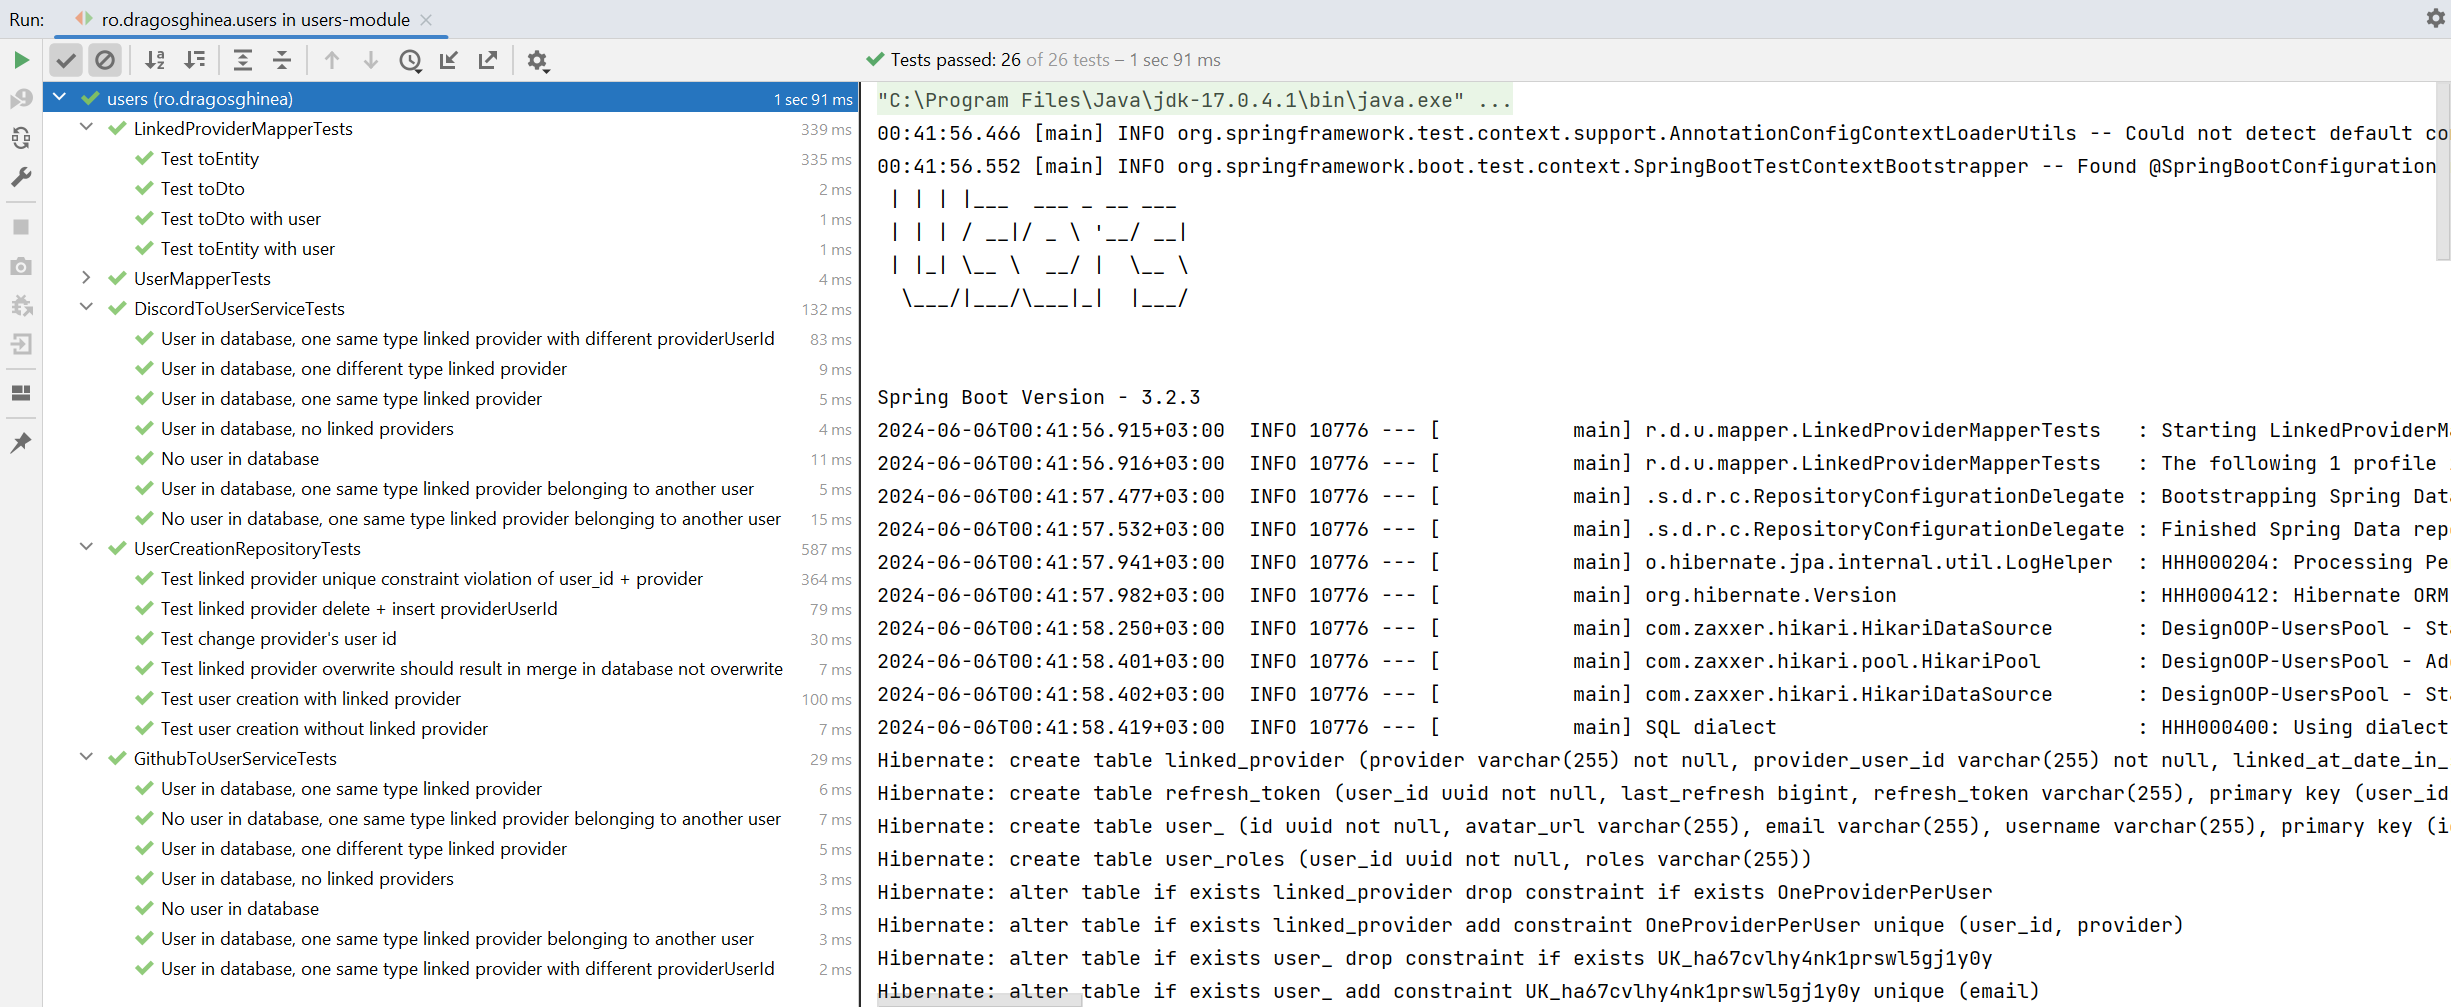
\includegraphics[trim={0 0 17cm 0},clip, width=\textwidth]{images/intellij-tests.png}
    \caption{Tests executed in IntelliJ IDEA}
    \label{fig:intellij-tests}
\end{figure}

\noindent \textbf{Postman} \cite{postman} serves as an API development tool enabling users to execute intricate requests and document them. Within this web platform, it was employed for manual route testing, involving tasks such as verifying correct request parsing, assessing response format, and inspecting backend side effects upon route access.

\begin{figure}[h]
    \centering
    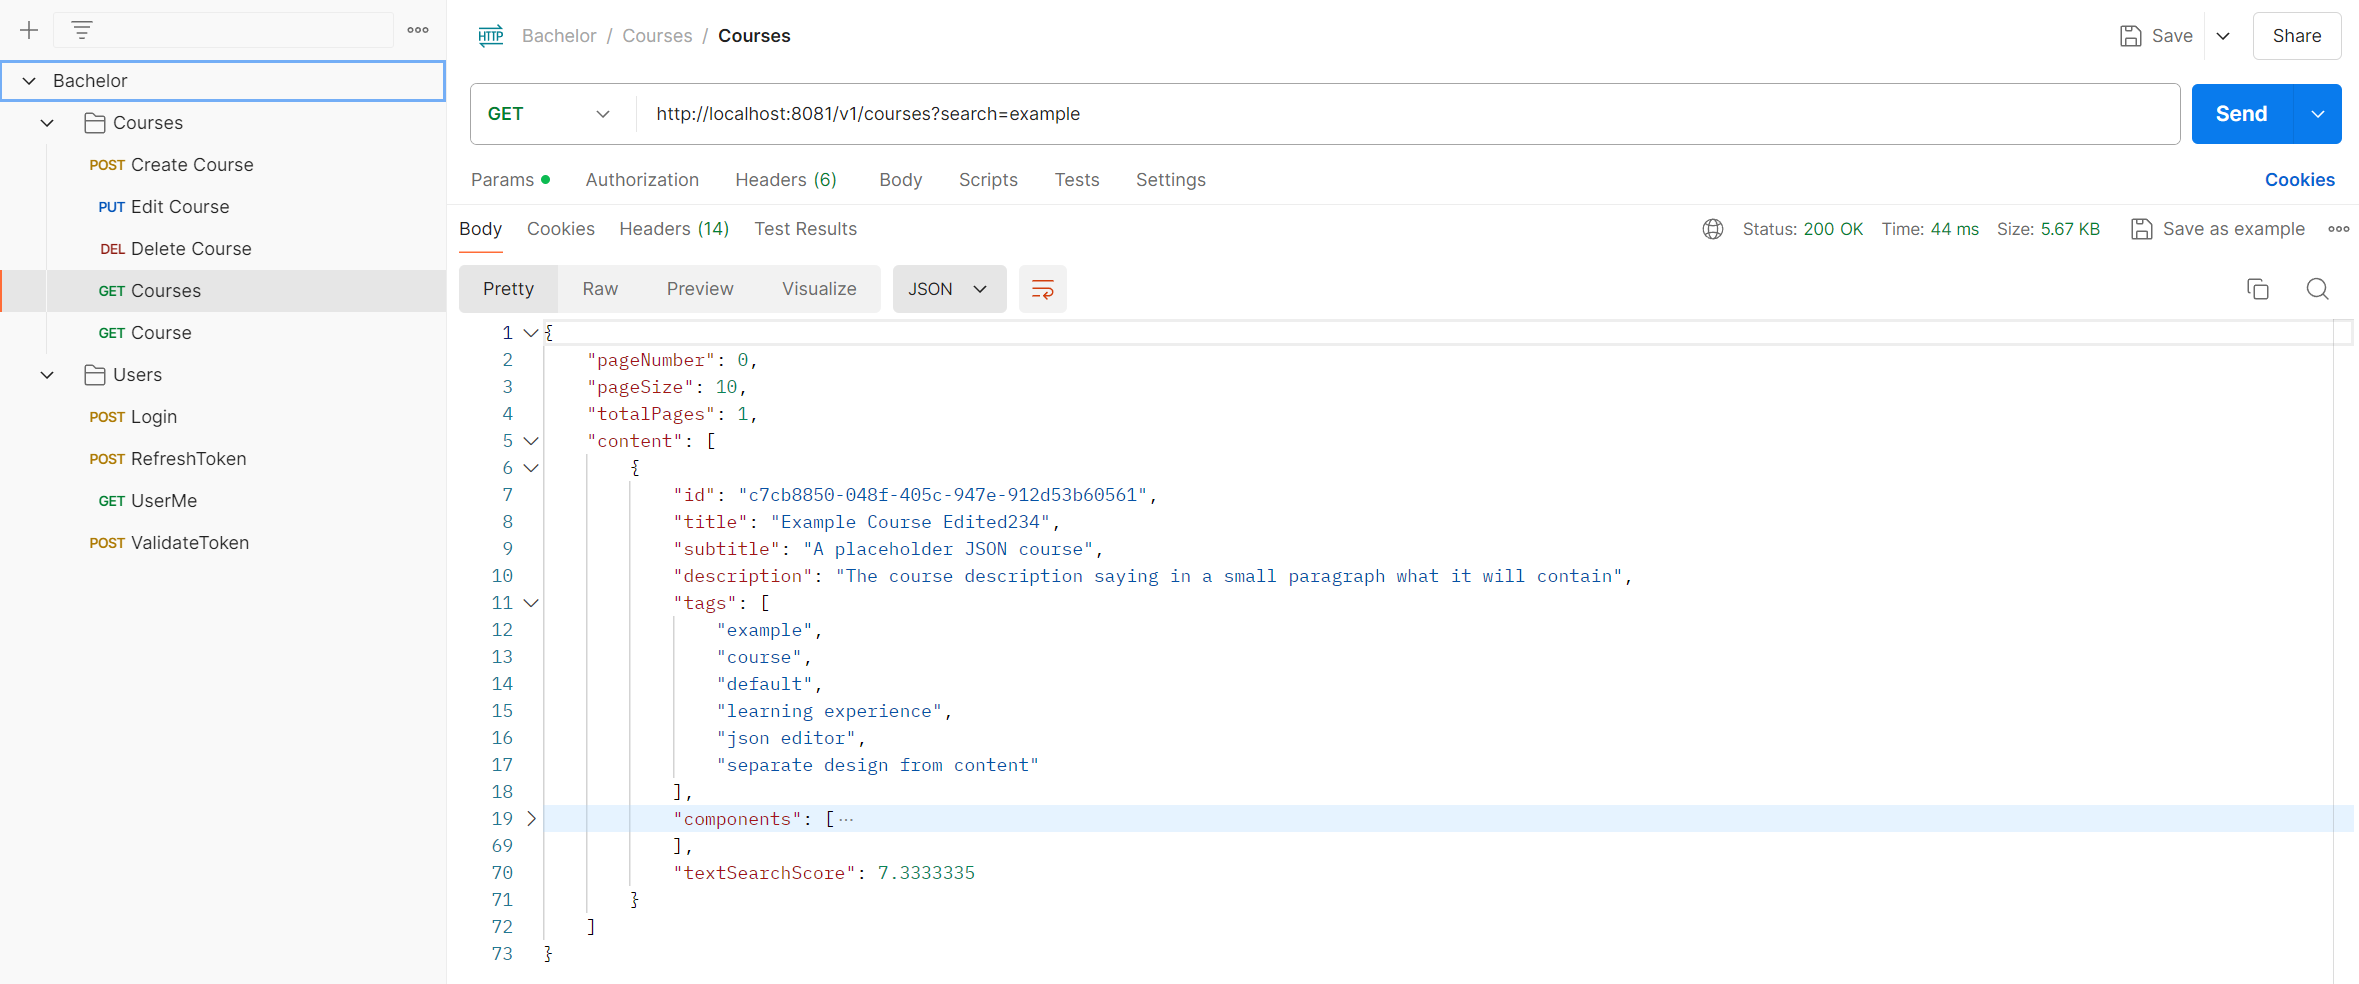
\includegraphics[trim={0 0 20cm 0},clip, width=\textwidth]{images/postman.png}
    \caption{Postman Interface}
    \label{fig:postman}
\end{figure}

\noindent In Figure \ref{fig:postman} the Postman interface is displayed, showcasing the collections and some requests used for testing the routes. The image also displays the response format for a successful GET request used to fetch the list of courses, using a search query. From the response, we can see that the courses are paginated and that each course has a text search score.
\\\\
\noindent In the future, Postman can also be used to document the API, as it provides features for adding descriptions and examples to collections and requests.
\chapter{Frontend Explained}

In this chapter I will document the contents of the frontend project and challenges met along the development process.

\section{Project Configuration}
\subsection{NextJS}

\noindent As discussed in the \textbf{Architecture and Choice of Technology} chapter, the frontend is built with NextJS 14. The project is configured to use TypeScript, Tailwind, ESLint, and the App Router.
\\\\
\noindent The App Router defines rules for creating routes within the application. For more details, see the project structure of an App Router application here \cite{nextjs-app-router-folders}. Although components can be placed directly in the App Router, only routes are placed inside it to maintain separation of concerns. While it was not possible to have separate app folders for each module, a minimum distinction is created by having different folders for each module inside the app folder, such as \textbf{main}, \textbf{(courses)}, and \textbf{(users)}. Folders with names in round brackets are interpreted as not being part of the route, thus providing only grouping capabilities.
\\\\
\noindent Throughout the application, environment variables are used to specify settings such as OAuth2 client secrets and other configuration variables needed throughout the application. Notably, these include the URLs to the backend modules, which can be accessed both in development mode and in production. NextJS by default allows the existence of three files: \textbf{.env.development}, which is used only in development mode, \textbf{.env.production}, which is used only in production, and \textbf{.env*}, which can override any value provided in the previous two files. There are also two types of environment variables within those files: private ones that are not accessible on the client side, ensuring they don't accidentally leak, and publicly available ones that are also added on the client side. To recognize a variable as a publicly available one, it needs to start with the prefix \texttt{NEXT\_PUBLIC\_}. \textbf{Attention!} It is important to take into account that \texttt{NEXT\_PUBLIC\_} variables are hardcoded and replaced with their values at project build time. This makes them immutable, so they should be properly set before the build. More information regarding how environment variables are handled by NextJS can be found here \cite{nextjs-env-variables}.

\subsection{VSCode + Extensions}

\noindent The coding environment utilizes VSCode with several helpful extensions. Custom configurations are added in the \textbf{.vscode} folder, inside a \textbf{settings.json} file, to tailor the project setup. To enhance development efficiency, the following extensions are employed: One Dark Pro, ESLint, npm Intellisense, Path Intellisense, Tailwind CSS Intellisense, Auto Rename Tag, Babel JavaScript, JavaScript and TypeScript Nightly, and Prettier. These extensions facilitate development by providing an aesthetically pleasing editor, offering suggestions for autocomplete and refactoring, highlighting potential syntax or logic errors in the code, and formatting all frontend code according to a customized standard. 
\\\\
\noindent The content of the \texttt{settings.json} file is presented below. It contains editor settings as well as extension settings that override the default ones.
\\\\
 \noindent The setting \textbf{"editor.defaultFormatter": "esbenp.prettier-vscode"} specifies Prettier as the default formatter for the editor, ensuring consistent code formatting. The setting \textbf{"editor.formatOnSave": true} enables automatic formatting of the code each time a file is saved. Under \textbf{"editor.codeActionsOnSave"}, \textbf{"source.fixAll.eslint": "explicit"} and \textbf{"source.addMissingImports": "explicit"} ensure that ESLint fixes all fixable issues and adds any missing imports when the file is saved. The \textbf{"files.associations"} section associates \texttt{.css} files with the Tailwind CSS language mode for better syntax highlighting and IntelliSense support. Various Prettier settings are defined to standardize the code style: \textbf{"prettier.tabWidth": 2} sets the tab width to 2 spaces, \textbf{"prettier.useTabs": false} ensures spaces are used instead of tabs, \textbf{"prettier.semi": true} enforces the use of semicolons, \textbf{"prettier.singleQuote": false} and \textbf{"prettier.jsxSingleQuote": false} enforce the use of double quotes for JavaScript and JSX respectively, \textbf{"prettier.trailing-\\Comma": "es5"} requires trailing commas where valid in ES5 (such as objects, arrays, etc.), and \textbf{"prettier.arrowParens": "always"} ensures parentheses are always used around arrow function parameters. For TypeScript React files, the default formatter is again set to Prettier with \textbf{"typescriptreact" : { "editor.defaultFormatter": "esbenp.prettier-vscode" }}.

\subsection{Tailwind}

\noindent Tailwind CSS is automatically integrated by NextJS, but further customization is done via \textbf{tailwind.config.ts}. Besides the configuration, custom styles are defined inside the \hl{/styles} folder. The main CSS file is \textbf{globals.css}, in which the other CSS files are imported. The \textbf{globals.css} file is then imported in the root layout of the frontend application. For this web platform, CSS files are mainly used to declare variables and add custom classes in one of the three layers of Tailwind: \textbf{base}, \textbf{components}, and \textbf{utilities}. The \textbf{base} layer is used for applying global styles and setting up foundational styles such as resets and typographic defaults. The \textbf{components} layer is for defining custom component styles, such as buttons and cards, ensuring consistency across the application. The \textbf{utilities} layer consists of utility classes that can be applied directly in the HTML to modify individual elements, providing a high degree of flexibility and control over styling. 
\\\\
\noindent The \textbf{tailwind.config.ts} file provides an easy way to extend the default theme and override or create new CSS classes. Besides extending the theme, the config file is used to specify the files that use Tailwind. The config file also allows the extension of Tailwind CSS with plugins, such as \textbf{tailwindcss-animate} and \textbf{@tailwindcss/container-queries}. These plugins enhance the functionality of Tailwind by adding additional utilities and features, making it more versatile and powerful for complex styling needs.

\subsection{Middleware}

\noindent In previous versions, I have referred to the backend created by NextJS as the middleware of the application. In this subsection, I am referring to the middleware configuration within NextJS, specifically the interceptor of requests between the client and the backend of NextJS. The middleware of this NextJS project is handled via the \textbf{middleware.ts} file. This file exports two main objects: a \textbf{NextMiddleware} function that receives a request and returns a NextResponse, and a \textbf{config} object which provides extra settings for the middleware. For example, the \textbf{config} object can define a pattern for matching routes, ensuring that not all routes will be affected by the NextMiddleware function. More information regarding the logic inside the auth middleware can be found in the security section.

\section{Folder structure}

In Figure \ref{fig:figure5}, the folder structure of the frontend project is presented. It is noticeable at first sight that some folders repeat themselves, appearing both at the root of the project and inside a module. This is intentional, as the folders have the same purpose wherever they appear. The difference between them is that the root folders are more general, meaning they can be used across all modules, while the nested folders are specific to the module they belong to.

\begin{figure}[h]
    \centering
    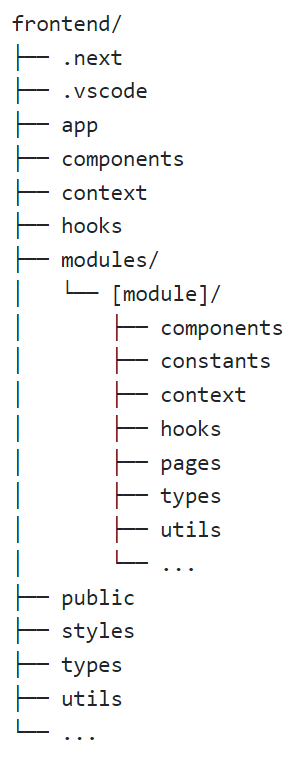
\includegraphics[scale=0.75]{images/frontend-folder-structure.png}
    \caption{Frontend - Folder structure}
    \label{fig:figure5}
\end{figure}

\noindent The \textbf{.next} folder contains bundled files essential for development mode, including cache of fetch requests and other metadata required for the NextJS project to function. Occasionally, I encountered random errors with the bundler, which were resolved by deleting this folder along with the \textbf{node\_modules} folder and allowing them to regenerate.
\\\\
\noindent The \textbf{.vscode} folder, previously discussed, contains the \textbf{settings.json} file, which specifies the extension properties to override in VSCode. This folder becomes completely unnecessary if a different text editor is used.
\\\\
\noindent The \textbf{app} folder is designated for NextJS's App Router and contains the folder tree that maps to various routes within the frontend application.
\\\\
\noindent The \textbf{components} folder contains reusable UI components that are used throughout the application. Components are the building blocks of the user interface, encapsulating markup, styles, and behavior. By organizing them in a dedicated folder, you ensure that they are easily accessible and can be reused across different parts of the application. This promotes consistency and reduces duplication. 
\\\\
\noindent The \textbf{hooks} folder contains custom React hooks. Hooks are functions that allow you to use state and other React features without writing a class. Custom hooks enable the reuse of stateful logic between components. By placing these hooks in a dedicated folder, the shared logic such as data fetching, form handling, or authentication is modularized and can be used across multiple components.
\\\\
\noindent The \textbf{context} folder is used for React Context API files. Context provides a way to pass data through the component tree without having to pass props down manually at every level. By using a context folder, global state or configuration that needs to be accessible throughout the application, such as theme settings or user authentication status, are managed and organized. This ensures that the context definitions and providers are centrally located and easy to manage.
\\\\
\noindent The \textbf{constants} folder contains constant values used across the application. By centralizing these values, the application ensures that they are defined in one place, making them easy to update and reducing the risk of hardcoded values scattered throughout the codebase. This practice improves maintainability and clarity, as developers can quickly locate and modify constants as needed.
\\\\
\noindent The \textbf{types} folder is dedicated to TypeScript type definitions. Type definitions help ensure that the code is type-safe, providing better tooling support, such as autocompletion and error checking. By placing important and reusable type definitions in a single folder, the NextJS project maintains a clear structure and make it easy to manage and reference types across the application. This is especially useful in large codebases where consistent use of types can prevent bugs and improve code quality.
\\\\
\noindent The \textbf{utils} folder contains utility functions and helper methods that are used across the application. These functions perform common tasks that are not specific to any single component or module, such as formatting dates, manipulating arrays, or making API requests. By organizing these utilities in a dedicated folder, it promotes code reuse and keep the codebase DRY (Don't Repeat Yourself). This also makes it easier to test and maintain these utility functions independently of the components that use them.
\\\\
\noindent The \textbf{modules} folder simulates a multi-module architecture, with each child folder representing a module that defines its own structure. Each module typically contains folders such as components, types, utils, constants, context, hooks, and pages. This design allows for modular development, where each module can independently specify its own folders or omit unnecessary ones. The \textbf{pages} folder, unique to each module and absent in the root structure, defines pages and layouts imported into the \textbf{app} folder. This structure ensures that each module is self-contained and can manage its specific functionality while maintaining a coherent overall project organization.
\\\\
\noindent The folder structure presented in Figure \ref{fig:figure5} and previously explained was inspired by the project structure of other applications, but mostly by this blog post \cite{react-folder-structure}.
\\\\
\noindent When referencing files within this folder structure, it is important to use absolute paths instead of relative ones. Although this approach might break modularity, as moving a folder will invalidate the paths within it, it provides clarity regarding the overall location of the imported files. The @/ symbol is used to denote the root of the application, simplifying the process of locating and importing files across different modules. This practice ensures that file references are consistent and understandable, regardless of the specific module or directory from which they are being accessed.

\section{Themes and Design}

\subsection{Light and Dark}

\noindent The web platform offers two main themes: dark and light. Additionally, there is a "system" theme that selects between dark and light based on the preferences of the user's device.
\\\\
\noindent These themes are implemented using the \textbf{next-themes} package from npm. This package provides a \textbf{ThemeProvider}, which is placed in the root layout of the application. CSS variables for theme customization are declared at the \textbf{@base} Tailwind layer, within the \textbf{:root} and \textbf{.dark} modifiers. These variables dynamically switch between light and dark modes based on the selected theme.
\\\\
\noindent The package also offers a \textbf{useTheme} hook, which allows retrieval of the selected theme and the resolved theme. The selected theme can be light, dark or system, but the resolved theme will be either light or dark, depending on the device settings. The \textbf{useTheme} hook also provides a \textbf{setTheme} function to update the theme. Importantly, the package ensures that if dark mode is enabled, the light theme will not flicker before the dark theme loads, providing a smooth user experience.
\\\\
\noindent To apply custom styles on components with Tailwind CSS now becomes very simple. All classes that are prefixed by \textbf{dark:} will be applied only on dark mode.
\newpage
\begin{figure}[h]
    \centering
    \begin{minipage}{0.45\textwidth}
        \centering
        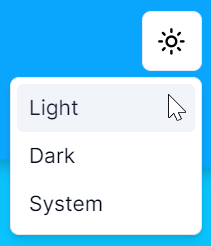
\includegraphics[width=0.5\linewidth]{images/theme-button-light.png}
        \caption{Theme Button - Light}
        \label{fig:theme-button-light}
    \end{minipage}%
    \hspace{0.1\textwidth}% 
    \begin{minipage}{0.45\textwidth}
        \centering
        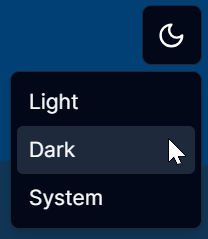
\includegraphics[width=0.5\linewidth]{images/theme-button-dark.png}
        \caption{Theme Button - Dark}
        \label{fig:ftheme-button-dark}
    \end{minipage}
\end{figure}

\noindent The user can easily change between themes using the button available on all pages, as shown in Figures \ref{fig:theme-button-light} and \ref{fig:ftheme-button-dark}. The button is implemented as a toggle switch, and will also change appearance based on the selected theme.

\subsection{Shadcn/UI}

\noindent Shadcn/UI is an open-source repository that offers accessible and customizable components implemented with \textbf{Tailwind CSS} and \textbf{Radix/UI Primitives}. Radix Primitives is a low-level UI component library focused on accessibility, customization, and developer experience. Shadcn \textbf{is not} a components library in the traditional sense, as components are not directly imported from a package. Instead, to use them, they need to be copy-pasted into the application, making the components as customizable as possible.
\\\\
\noindent The components taken from Shadcn \cite{shadcn-components} are placed in the \textbf{ui} folder within the root \textbf{components} directory. Although these components are fully editable, most are retained in their original source code with only minor modifications related to typography or the addition of extra variants. This approach ensures the components remain customizable while still adhering to the design standards of the application.
\\\\
\noindent The components provided by Shadcn integrate well with Next-Themes as well, having both light and dark modes.
\\\\
\noindent For installation, although the components can be manually copied, an automated option exists as well. Before using it, the \hl{npx shadcn-ui@latest init} command must be executed. This command configures download preferences for Shadcn, such as the components folder, TypeScript or JavaScript, CSS variables, component styles, and more. It also adds a utility function for merging multiple strings of classes, utilizing the \textbf{tailwind-merge} package, which is required within the source code of the components. After this initial setup, components can be downloaded via \hl{npx shadcn-ui@latest add <component>}.

\subsection{Typography}

\noindent Typography is an important aspect of the application, providing a subconscious user experience based on how it is chosen. The first step in defining typography was deciding on a typography scale. There are three main categories of typography scales: high contrast, medium contrast, and low contrast.
\\\\
\textbf{High Contrast:} This scale features significant size differences between text elements, making it ideal for drawing attention to headings and titles. It's useful for creating a dramatic and impactful design.
\\\\
\textbf{Medium Contrast:} With a balanced difference in text sizes, this scale is versatile and suitable for a harmonious and readable design. It works well for body text, subheadings, and captions, providing clear hierarchy without being overwhelming.
\\\\
\textbf{Low Contrast:} Featuring subtle size differences, this scale creates a uniform appearance and is perfect for minimalist designs. It enhances readability and user comfort, making it ideal for content-heavy applications like articles and reports.

\begin{figure}[h]
    \centering
    \begin{minipage}{0.45\textwidth}
        \centering
        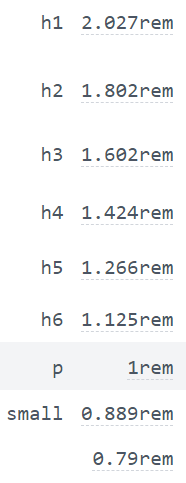
\includegraphics[width=0.5\linewidth]{images/typography-major-second.png}
        \caption{Major Second - 1.125}
        \label{fig:figure6}
    \end{minipage}%
    \hspace{0.1\textwidth}% 
    \begin{minipage}{0.45\textwidth}
        \centering
        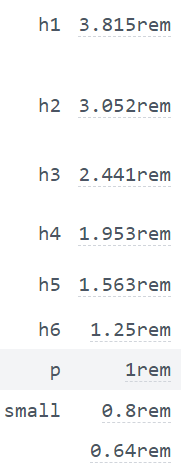
\includegraphics[width=0.5\linewidth]{images/typography-major-third.png}
        \caption{Major Third - 1.250}
        \label{fig:figure7}
    \end{minipage}
\end{figure}

\noindent For window sizes below \textbf{768px}, a major second typescale is applied, as depicted in Figure \ref{fig:figure6}. Conversely, for larger sizes, a major third typescale is utilized, as demonstrated in Figure \ref{fig:figure7}. Both fall within the \textbf{medium contrast} category, establishing a clear hierarchy while ensuring user engagement. % This approach facilitates distinct section separation while accommodating occasional heavier content.
\\\\
\noindent The typography scales mentioned above are implemented via custom Tailwind CSS classes (h1-typography, h2-typography, ..., p-typography, small-typography, caption-typography), which are directly applied to components. Occasionally, text size adjustments are made using Tailwind's text-[size] utility classes to improve page layout, but the overall design adheres to the specified scales.
\\\\
\noindent Adhering to NextJS's default settings, the web application adopts the \textbf{Inter} font. Alongside typography scale and font style considerations, factors such as letter and line spacing, color, and text decorators must be taken into account. Due to time constraints, emphasis has been placed on typography scale and font style, with other aspects being improvised to maintain an aesthetically pleasing design.

\subsection{Responsive}

\noindent Responsiveness is crucial for all web applications. Ensuring that a website looks good and works well on different devices and screen sizes is essential. Two strategies are employed inside the frontend application.
\\\\
\noindent Firstly, the web platform relies on Tailwind's responsive features, such as breakpoints for window sizes that conditionally activate classes when the minimum size is reached. Tailwind follows a mobile-first design approach, where styles are overridden from the smallest to the largest screen size.
\\\\
\noindent Secondly, a higher-order component is utilized to conditionally render content based on media queries. The \textbf{ConditionalRenderMediaQuery} component accepts three main parameters: \textbf{mediaQuery} (a string), \textbf{trueComponent} (a ReactNode), and \textbf{falseComponent} (a ReactNode). It can also receive additional parameters for server-side rendering configuration. This component leverages the \textbf{useMediaQuery} hook from the \texttt{usehooks-ts} library \cite{usehooks-ts}, which returns either true or false based on a media query string. Despite being marked as a client-side component, it can accept server-side components as parameters without converting them to client-side components. This is made possible by the inner workings of NextJS, which reserves slots for component parameters and renders the client-side component independently of the components received as parameters.
\\\\
\noindent An example of responsiveness can be seen in figures \ref{fig:main-page-desktop} and \ref{fig:main-page-mobile}, which display the different layout designs for desktop and mobile devices.

\section{Main Page}

The main page is designed to be minimalistic yet welcoming, with an attractive design and useful information. It focuses on transmitting three crucial pieces of information to the user:
\\\\
\noindent \textbf{Who are you?} This is conveyed through the web platform's logo and name, displayed in the navbar as DesignOOP. The name is suggestive and easy to remember, especially for courses related to object-oriented programming design patterns. The logo, generated with AI using \textbf{Bing AI}, represents building blocks surrounded by paintbrushes, signifying design.
\\\\
\noindent \textbf{What do you do?} This information is communicated through the suggestions card, which includes links to the community for user interaction, the official courses page, and the educational resources editor.
\\\\
\noindent \textbf{How can you help me?} This question is addressed through bullet points text on the main page, highlighting key benefits. Additionally, the suggestions card provides further assistance by offering relevant links and resources.

\begin{figure}[h]
    \centering
    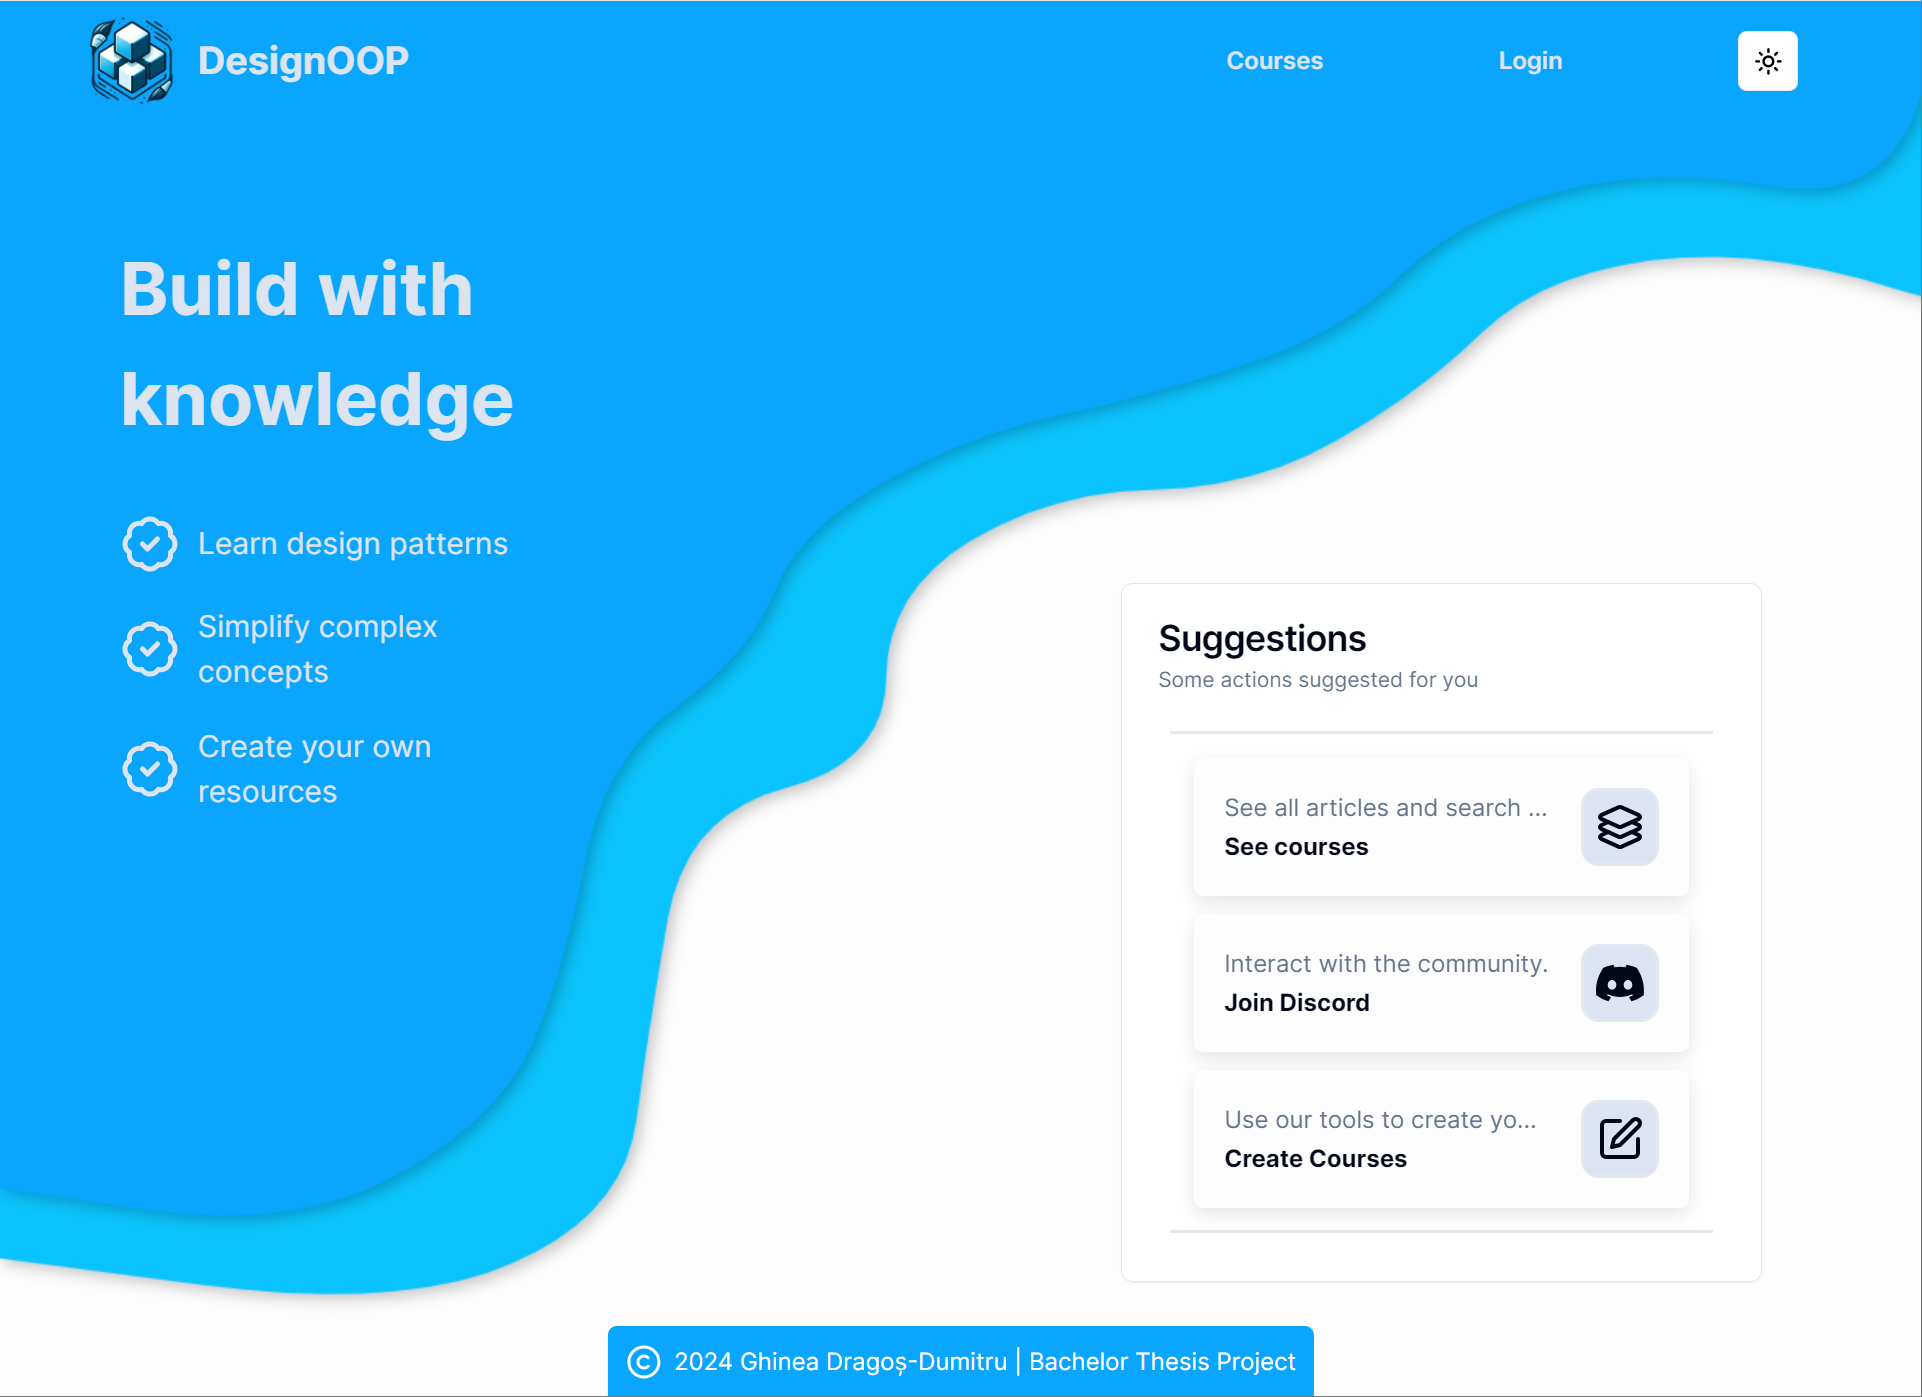
\includegraphics[scale=0.45, trim = {0 0 1 0}, clip]{images/main-page-desktop.png}
    \caption{Main Page - Desktop}
    \label{fig:main-page-desktop}
\end{figure}

\begin{figure}[h]
    \centering
    
\includegraphics[scale=0.4]{images/main-page-mobile.png}
    \caption{Main Page - Mobile}
    \label{fig:main-page-mobile}
\end{figure}

\subsection{Waves}

\noindent The wavy background with two layers is intended to create an organic, aesthetically pleasing look, providing a positive first impression of the application.
\\\\
\noindent When considering how to create the waves, \textbf{Bézier curves} were the first choice due to their ability to produce smooth and rounded lines. For the outline of the waves, cubic Bézier curves were utilized. Using an HTML canvas along with helper JavaScript functions to draw the curves and control points, a curve editor was created. This editor outputs the necessary control points to recreate the curve, with the coordinates normalized between 0 and 1, relative to the size of the canvas.
\\\\
\noindent The canvas shown in Figure \ref{fig:figure8} functions as a curve editor, allowing users to drag control points of multiple curves. The red dots indicate draggable control points, while the curves themselves are represented by green dots, placed closely together to form a continuous green line. In the canvas depicted, four Bézier curves are arranged next to each other, creating the appearance of a continuous wavy line. The canvas in Figure \ref{fig:figure8} has a square aspect ratio. For mobile waves, the same editing technique is employed, but instead of a square canvas, a slightly taller and narrower one is used. This adjustment ensures the waves are appropriately scaled and visually appealing on different screen sizes.

\begin{figure}[h]
    \centering
    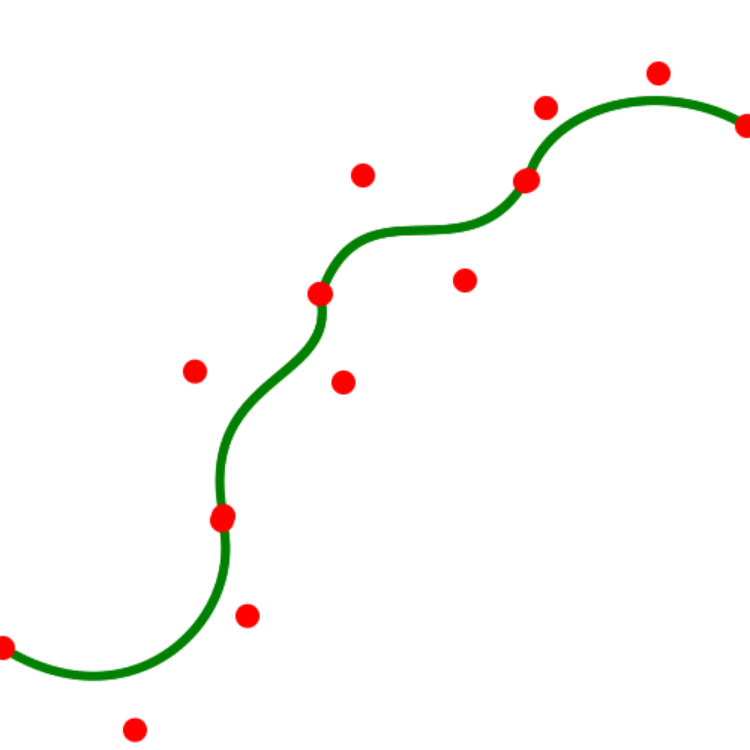
\includegraphics[scale=0.6]{images/bezier-curve-editor.png}
    \caption{Bézier curves in a canvas}
    \label{fig:figure8}
\end{figure}

\noindent After establishing the shape of the wave, the next step is to convert it into an actual surface. This is done by implementing the concept of \textbf{Bézier skin}. A Bézier skin is used on the main page to create a closed shape from Bézier curves based on control points. In Figure \ref{fig:figure9}, the control points are chosen as the top corners of the screen, to which the green dots are added. The green dots are generated along the curve established in Figure \ref{fig:figure8}. To make the wave move, the control points marked with green dots are moved diagonally back and forth, along a sinusoidal trajectory over time. For an organic feel, the dots are not moved back and forth simultaneously. To achieve a natural gradual randomization, \textbf{Perlin noise} is used.

\begin{figure}[h]
    \centering
    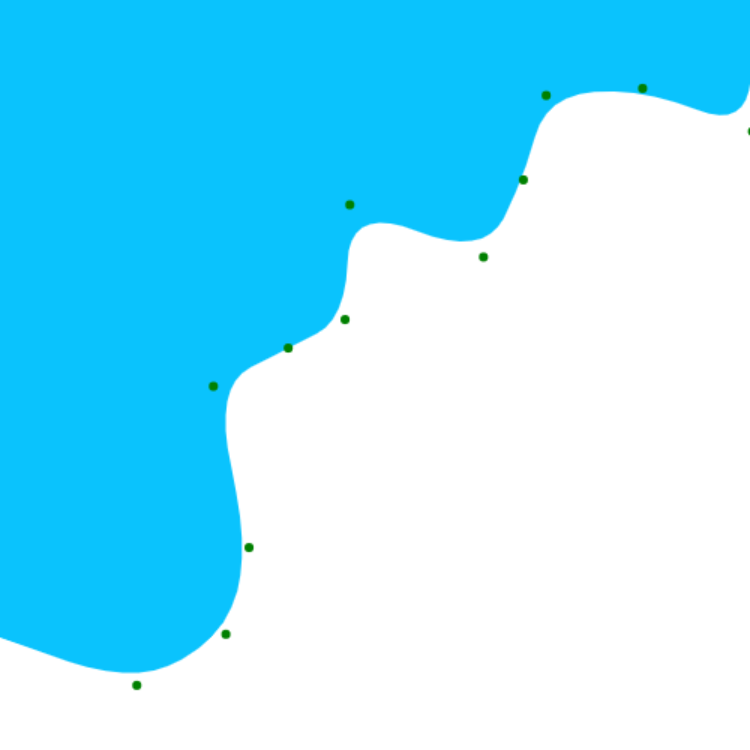
\includegraphics[scale=0.6]{images/bezier-wave-with-guides.png}
    \caption{Wave with guide points}
    \label{fig:figure9}
\end{figure}

\noindent After having the dynamic wave, the only thing left to obtain the final design is to add a shadow on it and combine it with another wave to offer depth perception. The final result is on the main page of the web platform.

\subsection{Navbar}

\noindent The navbar of the web platform contains multiple elements for quick access to other areas of the website. Firstly, there is the logo along with the web platform's name, which acts as a home button when clicked, loading the main page. Secondly, there is the courses button, which redirects to the courses section. Finally, there is the user profile button. If the user is not logged in, the button displays "Login"; for logged-in users, there are two buttons: one for accessing their profile and another for logging out.
\\\\
\noindent The navbar uses the \textbf{ConditionalRenderMediaQuery} higher-order component to selectively load a mobile navbar and a desktop navbar. The navbar component is not placed at the root level of the application but inside the layout of each module. Although the navbar might vary in design from section to section, it maintains a consistent look across all of them.
\\\\
\noindent To avoid the use of too many files, if the navbar requires a different style for a specific module of the application, a new variant is created, and Tailwind class names are added or removed accordingly. Currently, two variants exist: \textbf{main} (see Figure \ref{fig:navbar-main}) and \textbf{default} (see Figure \ref{fig:navbar-default}). If no variant is specified when the component is called, the default variant will be used.

\begin{figure}[h]
    \centering
    
\includegraphics[scale=0.55]{images/navbar-main.png}
    \caption{Navbar - Main Variant}
    \label{fig:navbar-main}
\end{figure}

\begin{figure}[h]
    \centering
    
\includegraphics[scale=0.55]{images/navbar-default.png}
    \caption{Navbar - Default Variant}
    \label{fig:navbar-default}
\end{figure}

\subsection{Suggestions}

\noindent The suggestions card currently directs users towards the three main uses of the application. Firstly, the \textbf{Join Discord} option connects users to a Discord community where they can interact with others who share an interest in design patterns and exchange knowledge. Secondly, the \textbf{See courses} option presents users with the official learning resources available on the web platform. Finally, the \textbf{Create courses} option redirects users to the educational resource creator, personalized in the style of the web application.
\\\\
\noindent A suggestion inside the suggestions box (Figure \ref{fig:suggestions-card}) consists of three components: a bolded title, a suggestive icon, and a description that is truncated but becomes fully visible on hover.

\begin{figure}[h]
    \centering
    
\includegraphics[scale=0.7]{images/suggestions-card.png}
    \caption{Suggestions box with hovered suggestion}
    \label{fig:suggestions-card}
\end{figure}

\noindent Although currently static, the suggestions could become more dynamic and user specialized in the future, by storing the user activity in their profile and recommend specific courses based on the visited ones.

\section{Profile}

The profile is part of the \textbf{users module}, along with the frontend security measures that will be covered in a later section.

\subsection{Details}

\noindent A user profile currently consists of their details (Figure \ref{fig:profile-card}). The profile page presents the avatar of the user along with their username, the linked providers, and the date they were connected. At the time of writing this thesis, there are two possible user providers: \textbf{Discord} and \textbf{GitHub}.
\\\\
\noindent Users are generated based on the emails from provider connections. If a user connects via GitHub, for example, with a specific email, and there is a user associated with that email, then the authentication request will resolve using that user. In case a user does not exist with that email, a new one is created and linked to the provider that resulted in the creation of the user. The initial profile picture along with the username are taken from the linked provider on user creation. If a linked provider changes their email, the linked provider's ID from the backend is automatically relocated to the new email.

\begin{figure}[h]
    \centering
    
\includegraphics[scale=0.7]{images/profile-card.png}
    \caption{Profile details card}
    \label{fig:profile-card}
\end{figure}

\subsection{Account Usage}

\noindent Currently, the accounts have only administrative purposes, being used for authorization. Authorization is required in the web application for course management. Although the course editor is open for everyone, even unauthenticated users, official courses can't be managed by anonymous people.
\\\\
\noindent In the future, accounts might serve an important role in managing data such as browsing history, which could facilitate a recommendation algorithm personalized to user preferences and needs. Besides that, a notifications center can be employed, providing users with direct messages if there are problems, opportunities to learn, or other things specific users might need to know. In the ecosystem of interacting with users, the possibilities are nearly endless.

\section{Courses}

The courses represent the main reason this web application exists. The frontend needs to provide valuable interfaces, both for reading the courses and creating them. To improve the user's experience multiple features are implemented, which are presented in the following subsections.

\subsection{Layout}

\noindent All pages from the courses module have a three-column layout, including as much information as possible in a structured way that is easily understood by people. On mobile, similar to this layout, only the middle section is displayed, but arrows on the sides of the screen allow the opening of the hidden sections as side sheets/dialogs. On top of this three-column layout is the global navbar of the application, refered to as the \textbf{static navbar}.
\\\\
\noindent The \textbf{left side} is a separate vertical navbar with specific options for the courses module. From this navbar, you can change between searching for courses, viewing your browsing history, and opening the course editor. The left side is meant to be somewhat generic for all pages from the module, but due to possible future extensions, the internal structure allows overwriting this navigation bar in any courses route.
\\\\
\noindent The \textbf{middle side} represents the most important content of the page you are on. For course searches, it will be a list along with a search bar. For a course view, it will be the content of the course. For a course editor, it will be a JSON editor for the components of a course, and so on.
\\\\
\noindent The \textbf{right side} should be a helper view to the main content presented in the middle side. For example, for a course view, it contains the table of contents and possible actions, such as opening it in the course editor. For the course editor, it offers a live preview of the components configuration. For course searches, it offers a search history.
\\\\
\noindent A \textbf{dynamic layout} is employed to give users more control over the size of the sides. The \textbf{react-resizable-layout} npm library is used to make each side a resizable box. A maximum and a minimum size are put on each side, so the user doesn't end up losing a section by making it disappear.
\\\\
\begin{figure}[h]
  \centering
  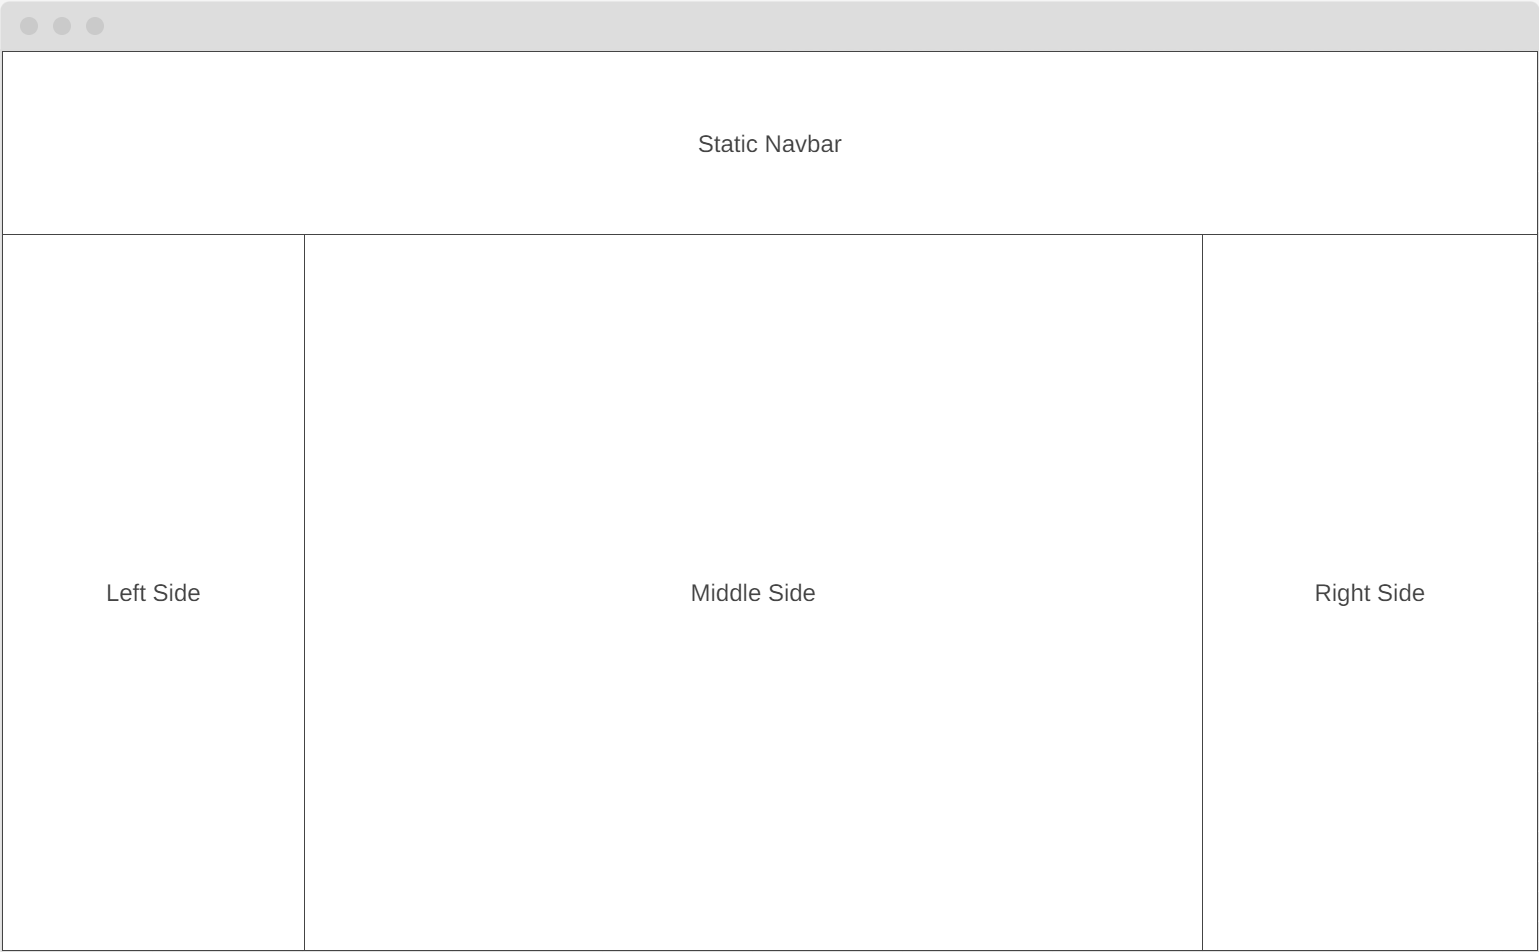
\includegraphics[scale=0.6]{images/courses-layout.png}
  \caption{Courses Module Layout - Desktop}
  \label{fig:figure10}
\end{figure}

\subsection{Search}

\noindent The search page is used for course navigation, presenting a general list of courses and the possibility to search through them. How the search input is parsed to produce the returned list of courses is explained in the backend chapter. In this subsection, the presented information for the user is explained. The components presented below can be seen in Figure \ref{fig:search-page}.
\\\\
\noindent Courses are displayed to the user in the format of cards. A course card consists of the title and subtitle, with the course description and the course tags. This information should be enough for identifying the course, and more details about it can be obtained by clicking it, which will open the course view. There is a height limit put on the description, so in case it gets exceeded, the content will become scrollable.
\\\\
\noindent The card also contains a search score when the search input is not empty. The score represents how likely the course is what the user was searching for. Although it theoretically is a score between 0 and 100, a 100 score is impossible, since you would need to search for everything present in the course to get it. The score is still relevant through relativity, as it can be used to order courses from the search. The course that has the higher score in a search is most likely more relevant than one with a lower score.
\\\\
\noindent While the middle side contains the search bar and the list of courses, the right sidebar contains a search history. Currently, the search history is saved inside \textbf{localStorage} and has a maximum of 10 entries. Older entries are automatically removed. All entries can, in fact, be removed through a clear all button that will empty the search.
\\\\
\noindent The search history is updated on each input change from the search field, but to avoid updating the history on each letter change, the \textbf{useDebounceCallback} hook from \textit{usehooks-ts} is used \cite{usehooks-ts}. The hook waits for half a second before signaling the input value change. If in the meantime a new value change event is triggered, then the waiting event is canceled, and the new event will also begin to wait. Eventually, the wait finishes without other events being triggered, and that is when the callback that has been waiting finally executes.
\\\\
\noindent In case there are no search results or the search history is empty a proper message is shown so the user is aware it is in fact not a loading error or broken display, and indeed there was nothing to show for their input. 

\begin{figure}[h]
    \centering
    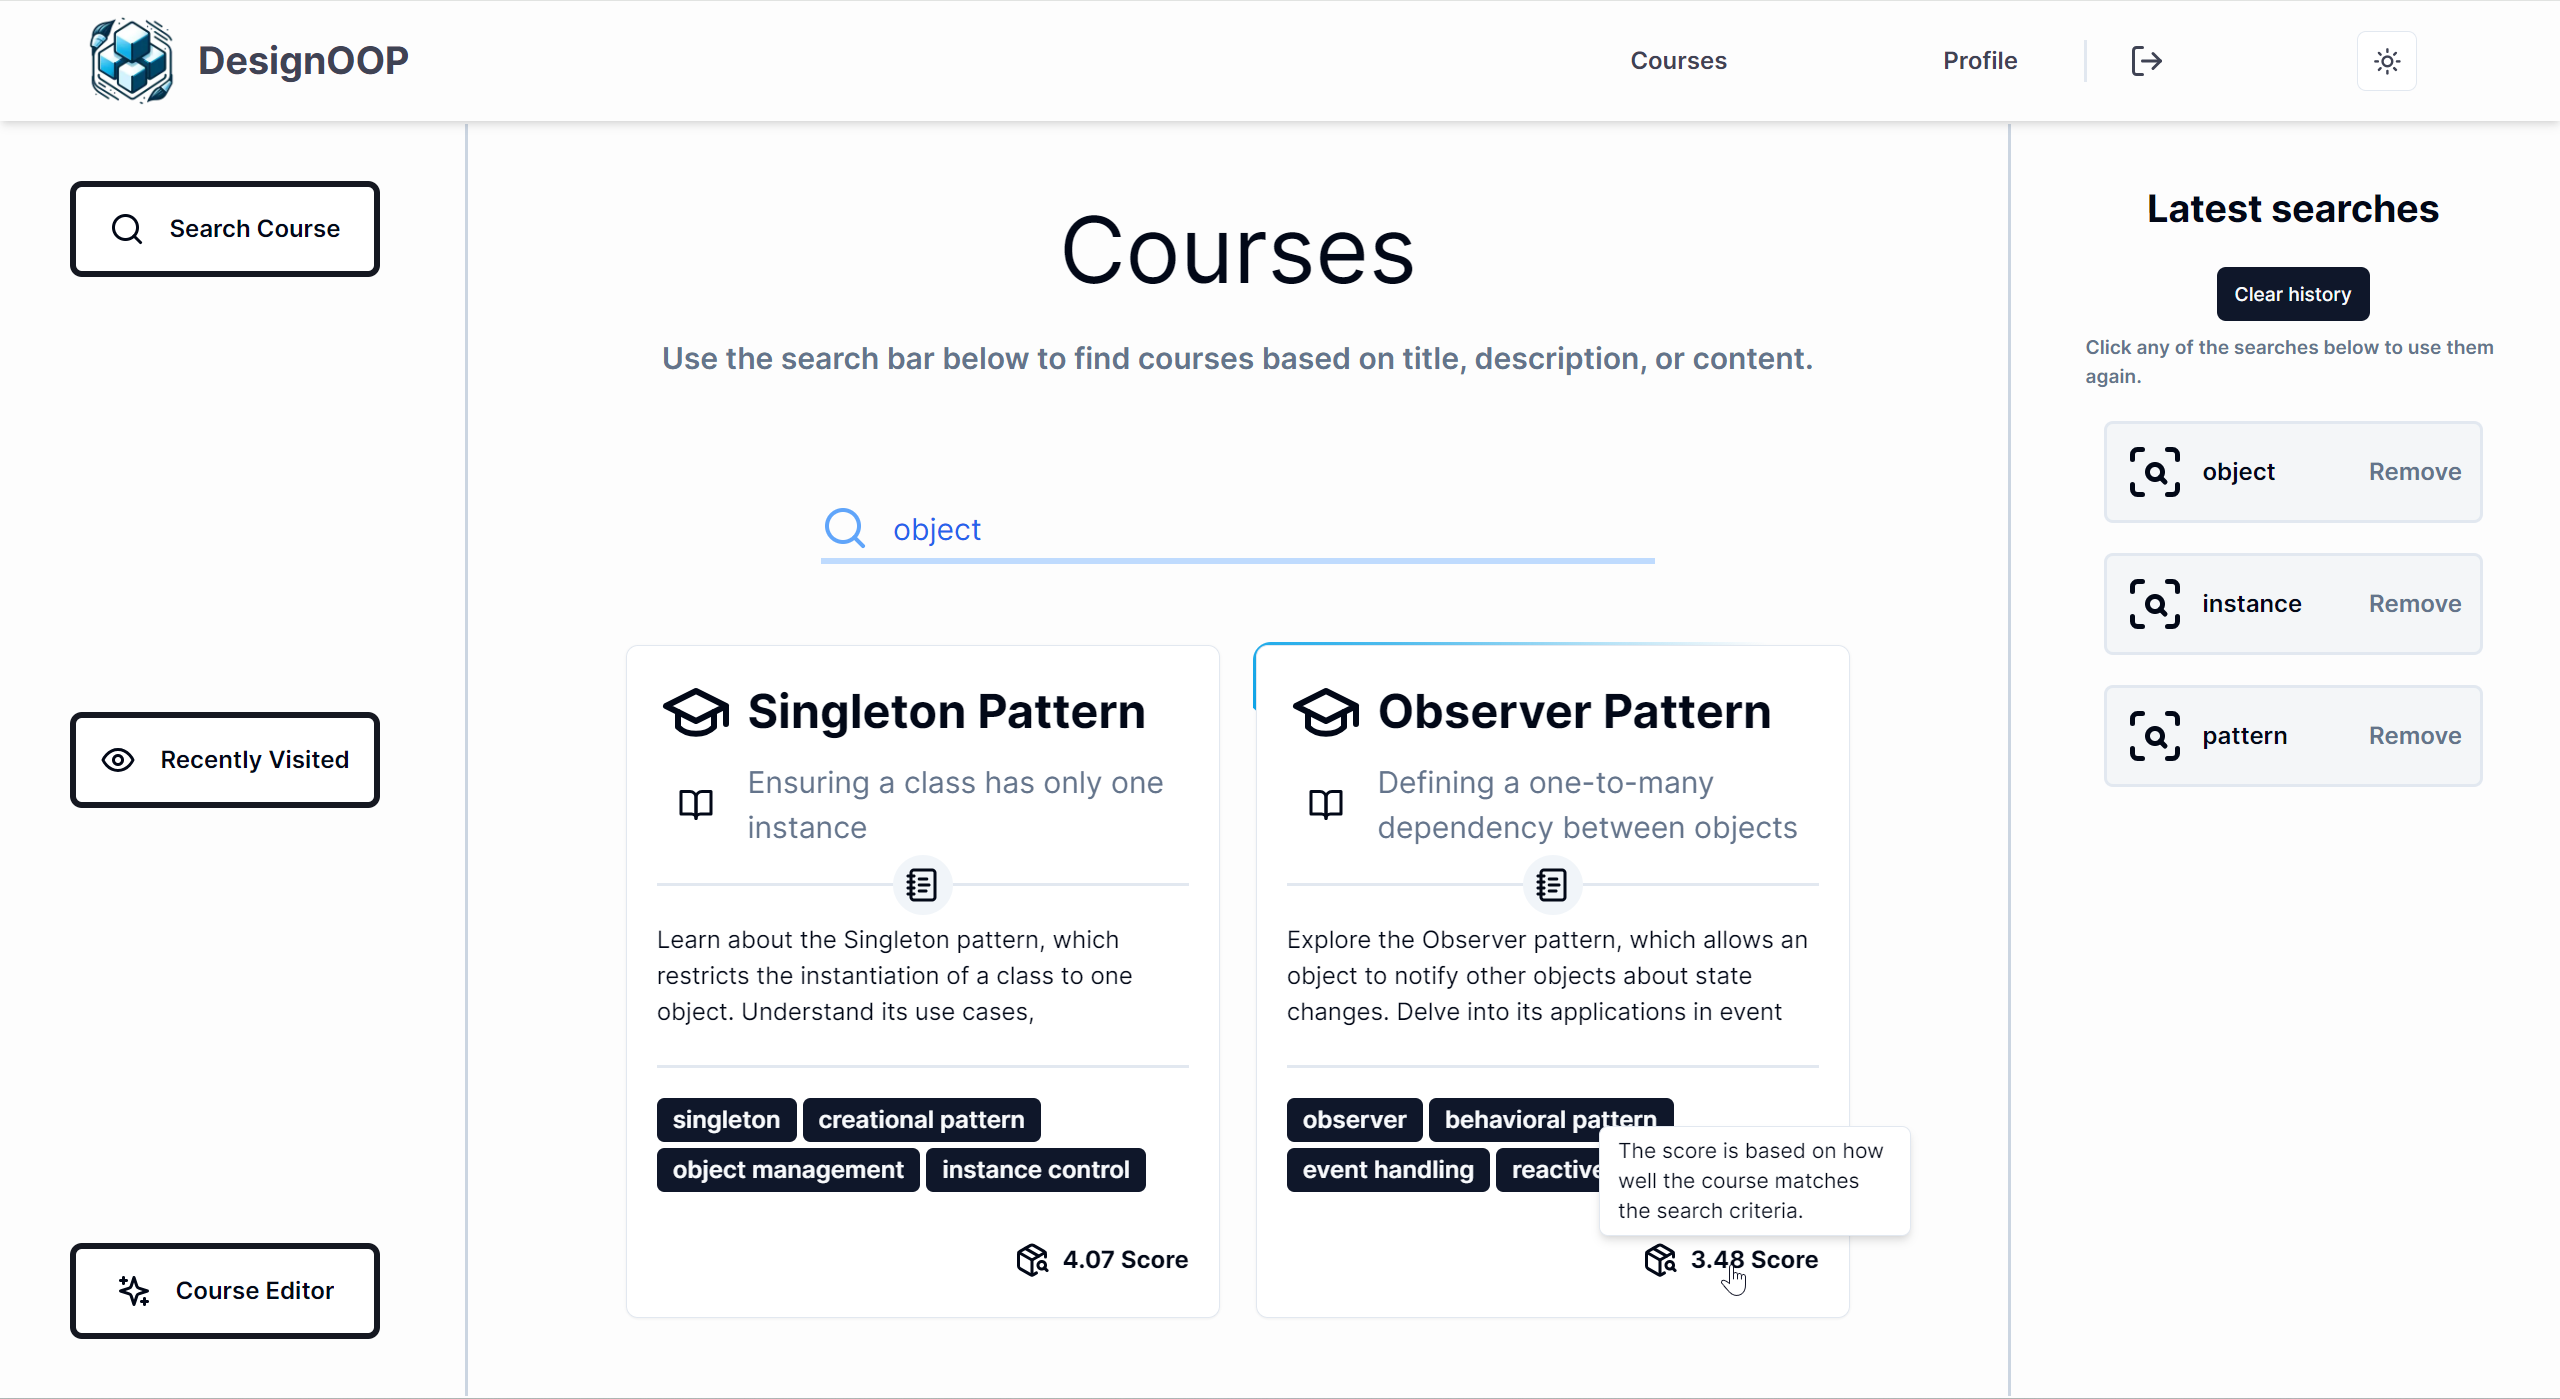
\includegraphics[scale=0.33]{images/search-page-preview.png}
    \caption{Courses search page}
    \label{fig:search-page}
\end{figure}

\subsection{Browsing History}

\noindent The course browsing history is also stored inside the \textbf{localStorage}. When entering a course page, a component used specially for side effects named \textbf{CourseViewHistory} uses the \textbf{useLocalStorage} hook from \textit{usehooks-ts} to update the browsing history of the \textbf{localStorage}. To avoid trips to the database, the information needed to output the course inside the history is saved completely.
\\\\
\noindent A \textbf{CourseHistoryItem} refers to the information needed to display a visited course. It contains the same information as a course card from the \textbf{Search} subsection, to which the search score is replaced with a last visited date. Since the course card is saved fully, even if the course information changes or is deleted, the display at which the course was accessed will be preserved.
\\\\
\noindent While the middle side displays the history, the right side presents the user with extra actions that they could take regarding it. Currently, the user can only clear their browsing history, but in the future, course recommendations might be placed here as well.
\\\\
\noindent When the browsing history is empty, a message telling the user that the page will be populated after some courses are accessed is displayed.

\begin{figure}[h]
    \centering
    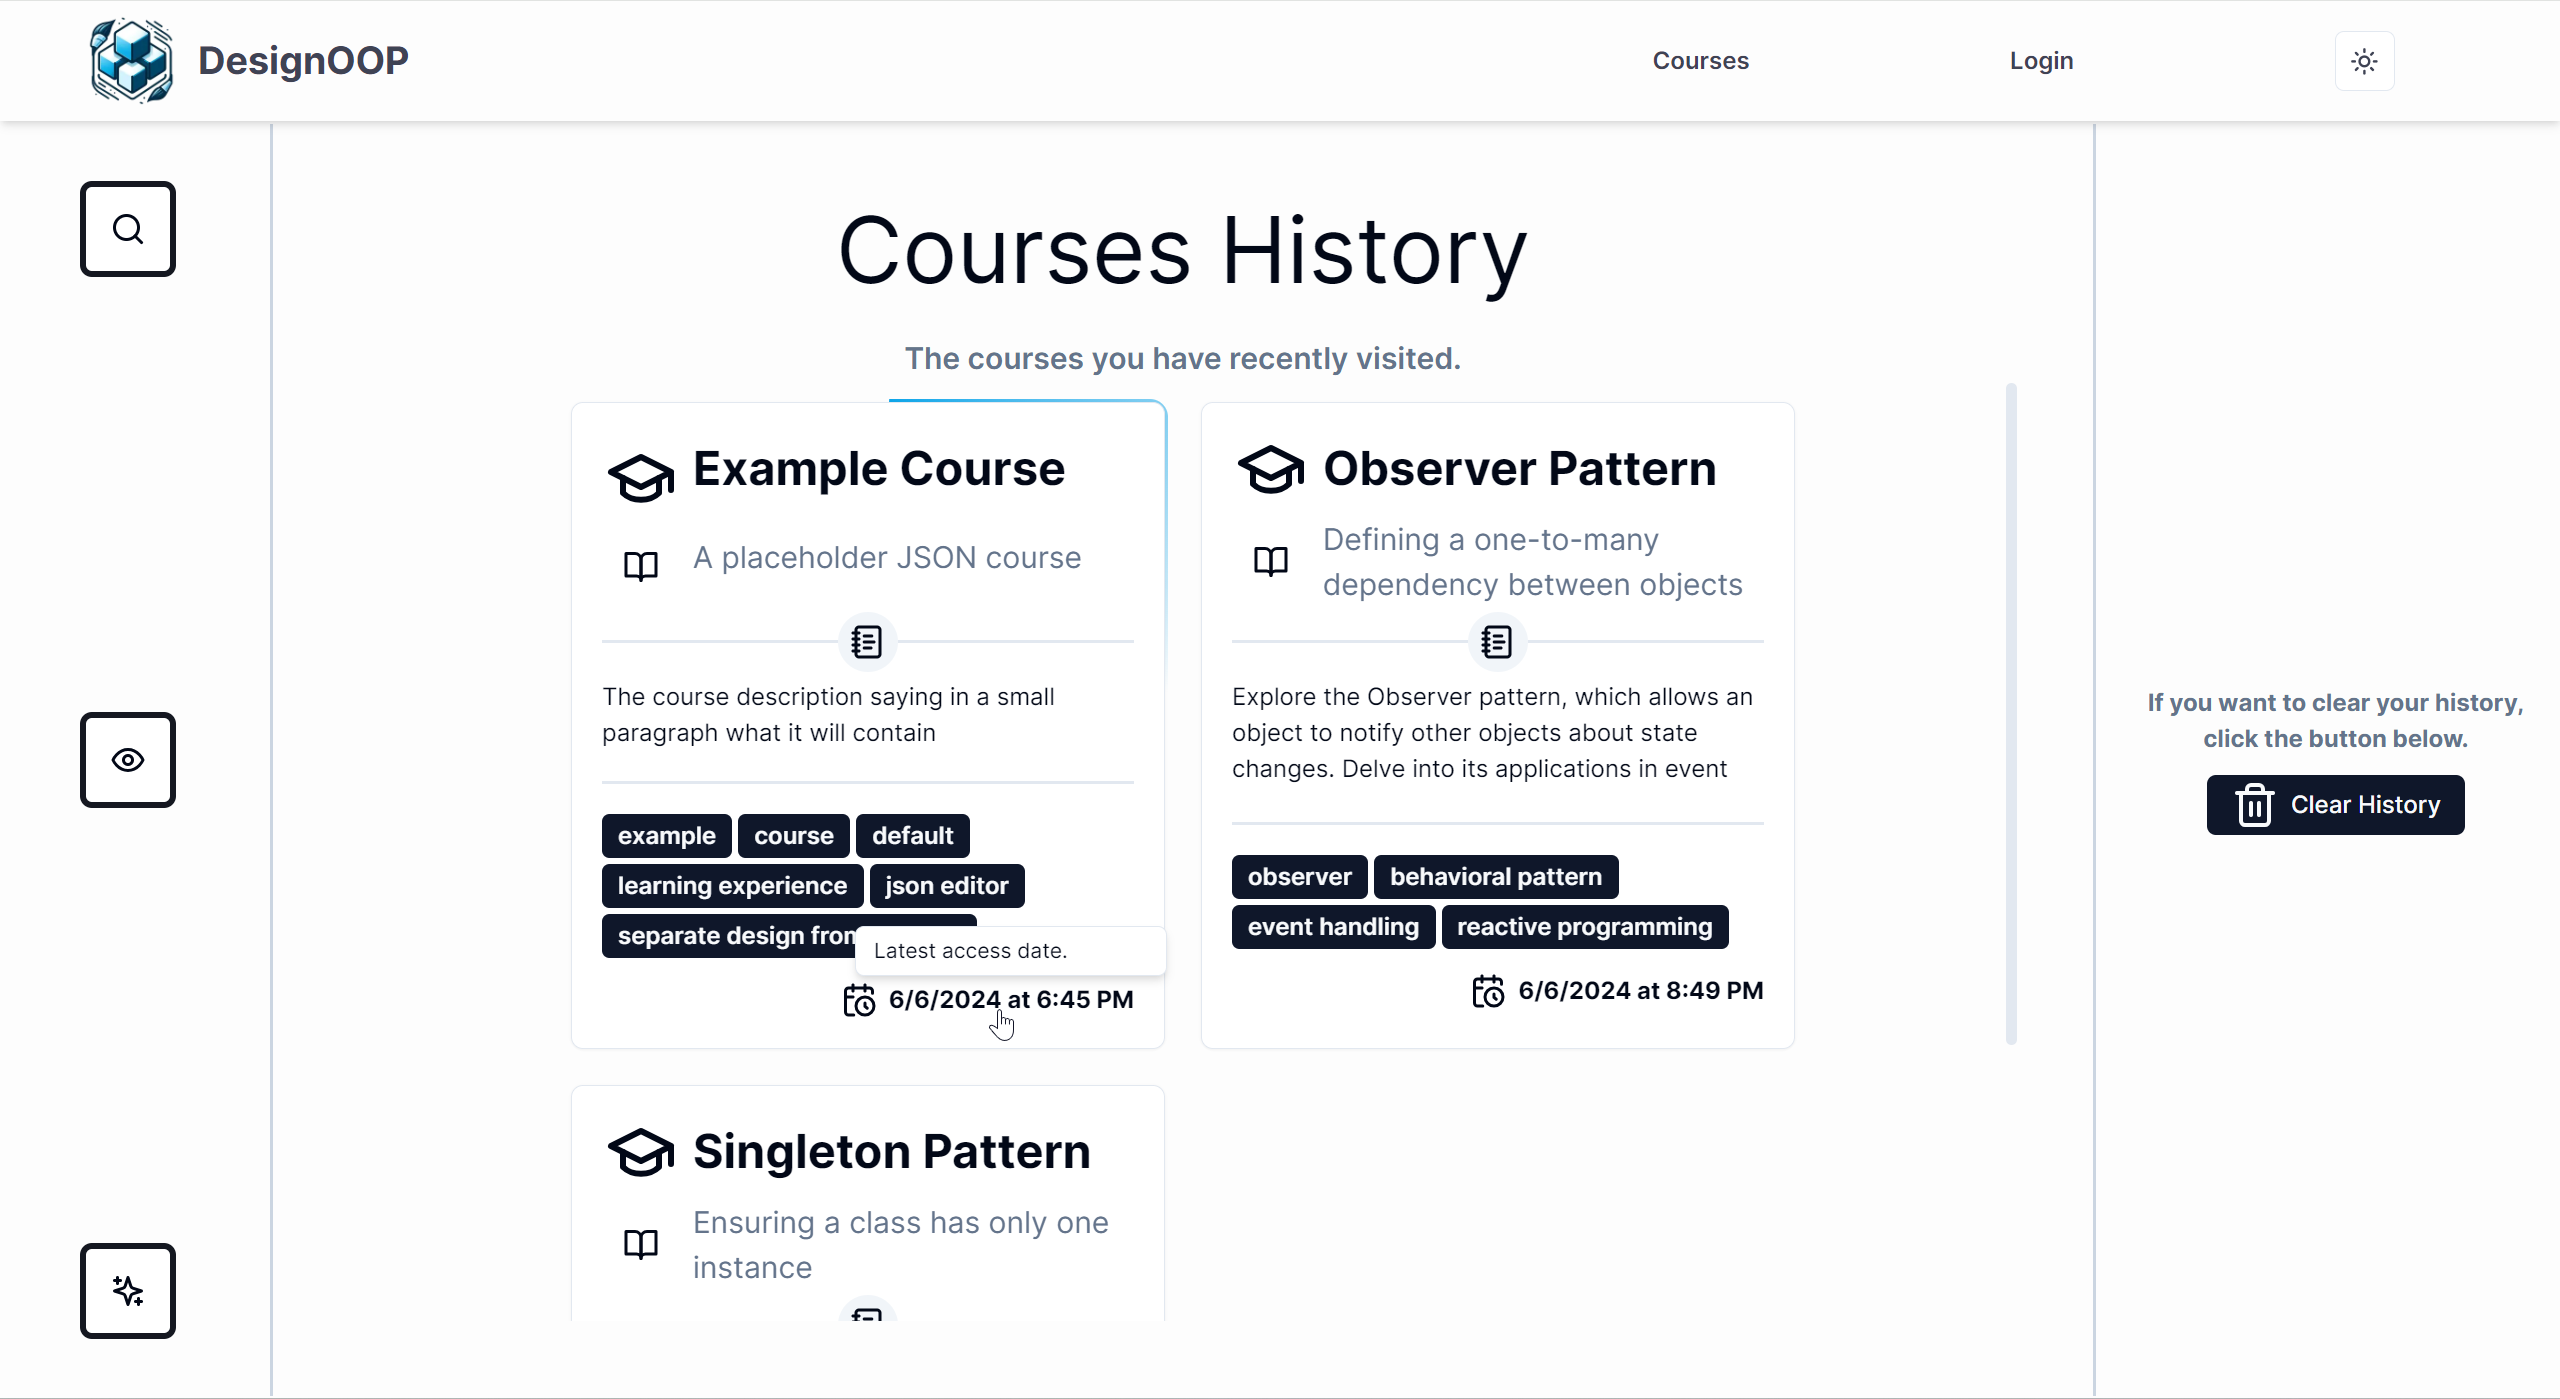
\includegraphics[scale=0.33]{images/courses-history.png}
    \caption{Courses browsing history page}
    \label{fig:courses-history}
\end{figure}

\subsection{View}

\noindent The course view loads the course in the middle section and utilities in the right side, such as a table of contents that helps navigation through the course's components (see Figure \ref{fig:course-table-of-contents}). Besides the table of contents, user actions are declared on the right side. Based on the authorization of the user, the actions could include a delete course button. To ensure it was not clicked by accident, a dialog will open that asks the user to type the name of the course to confirm deletion. Regardless of user authorization, a button for opening the course inside the course editor is shown to encourage users to create their own resources and learn from already written examples.
\\\\
\noindent In case the course can't load due to reasons such as an invalid courseId format, course not found, or unknown errors, the middle and right sides will display an appropriate error message.

\begin{figure}[h]
    \centering
    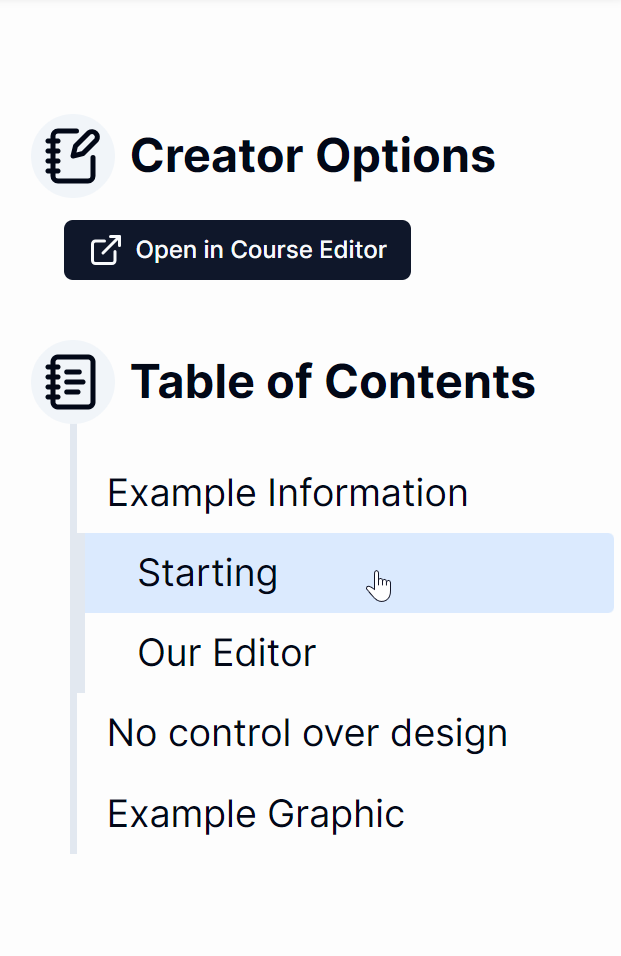
\includegraphics[scale=0.7]{images/table-of-contents.png}
    \caption{Course View - Right Side}
    \label{fig:course-table-of-contents}
\end{figure}

\section{Course Editor}

Although the course content is kept separate from the design, its internal structure can get very complex and intricate. Editing it in a usual text or code editor might prove challenging, as the most you can get out of them is syntax highlighting for JSON and autocompletion of brackets. For this reason, the web platform implements its own editor tool that can help the creator in a more specific way.

\subsection{Course Structure}

\noindent A \textbf{Course} component will parse the metadata of the course, along with the components tree, which is recursively parsed by \textbf{DynamicCourseComponent}.
\\\\
\noindent The \textbf{components} property of the course consists of multiple objects that can have dynamic parameters. For identifying them, all components must have the \textbf{componentType} property. In a separate \textbf{dynamic-course-components.tsx} file located inside the \hl{@/modules/courses/constants} folder, a \texttt{Components} constant object is declared. This constant maps a string to a configuration that contains three properties: \textbf{component}, \textbf{params}, and \textbf{hasChildren}. The \textbf{component} property returns a React component. The string that maps to this configuration is none other than the value of the \textbf{componentType} property.
\\\\
\noindent After the component configuration is identified using the raw JSON object, the \textbf{DynamicCourseComponent} will take the other properties of the object, with the exception of the \textbf{children} and \textbf{contentTable} properties, and pass them as parameters to the React component from the configuration. Using \texttt{useMemo}, the \textbf{children} property is parsed into a list of more dynamic components, therefore creating the recursive part. The usage of this hook ensures that the children are not rendered again unless the JSON object changes.
\\\\
\noindent All course components can be found inside the \hl{@/modules/courses/components/course/components} folder. If a new component is created or the parameters are modified, the \texttt{Components} constant also needs to be modified to reflect the changes.
\\\\
\noindent Each dynamic component is wrapped into an \textbf{ErrorBoundary} component, which will try to catch rendering errors as soon as they appear. This is especially useful in mid-editing, when components might not be written properly but you still want to be able to see the parts that work. The \textbf{ErrorBoundary} simply replaces the content with an error message.

\subsection{JSON Editor}

\noindent The JSON Editor is meant to fit the role of a code editor, specialized for creating resources that respect the format of this web platform. To achieve this, the \textbf{CodeMirror} library \cite{codemirror} was used. Since it is a JavaScript component, it cannot be used directly in React, as it needs to be wrapped inside a component. To do this, the web platform uses an already existing React wrapper over CodeMirror, \textbf{react-codemirror} by uiw \cite{react-codemirror}.

\begin{figure}[h]
    \centering
    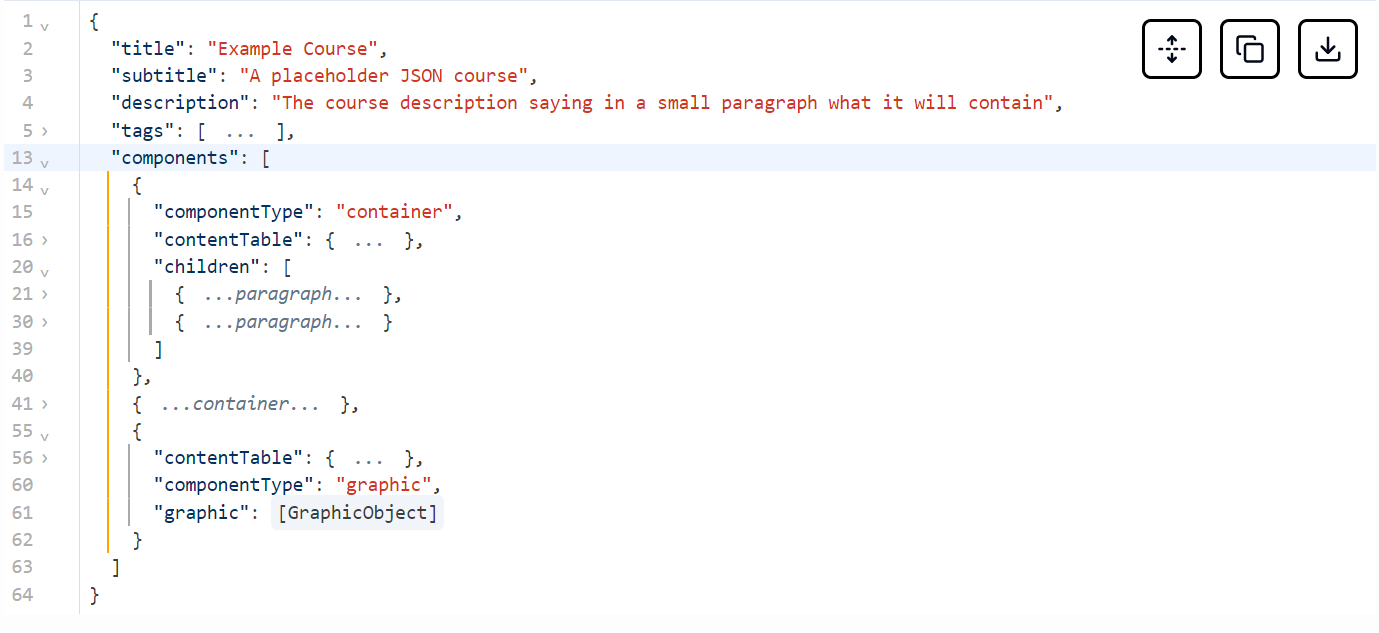
\includegraphics[scale=0.63]{images/json-editor-light.png}
    \caption{JSON Editor with example course - Light Theme}
    \label{fig:json-editor-light}
\end{figure}

\begin{figure}[h]
    \centering
    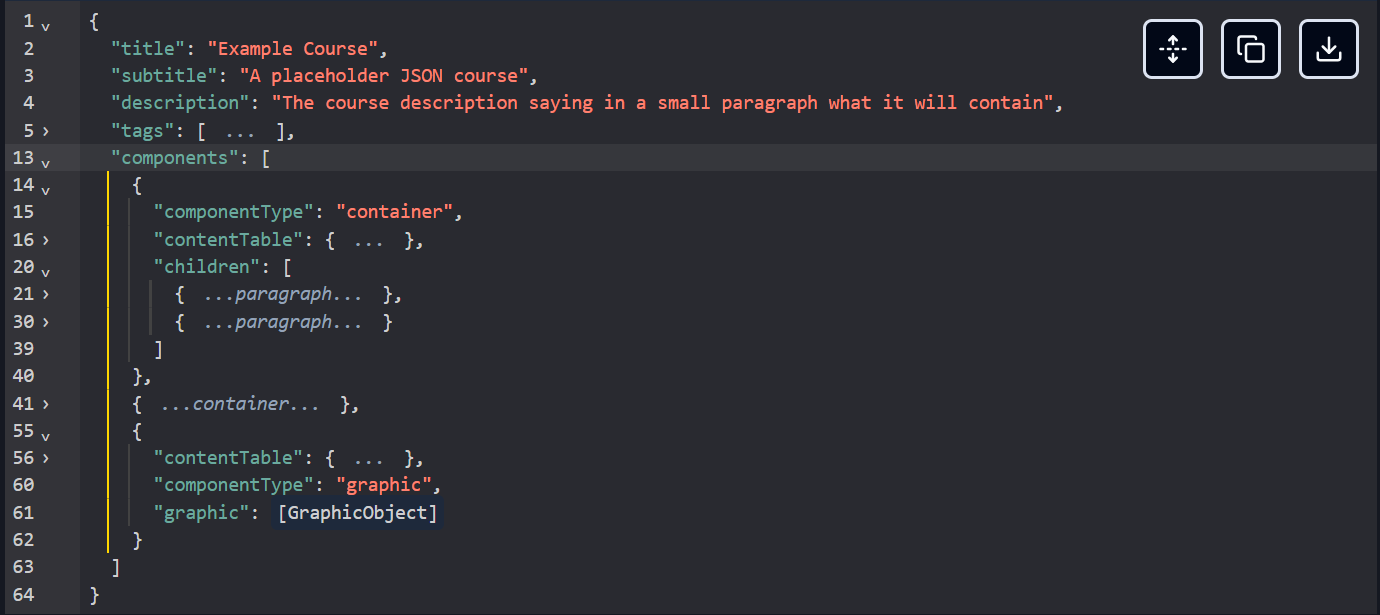
\includegraphics[scale=0.63]{images/json-editor-dark.png}
    \caption{JSON Editor with example course - Dark Theme}
    \label{fig:json-editor-dark}
\end{figure}
\newpage
\noindent The JSONEditor component is responsible for bringing together all the custom features that make the code editor functional. Firstly, it returns a react CodeMirror instance, to which a JSON content is passed as initial value. For syntax highlighting, the \texttt{lang} parameter is set to "json". The CodeMirror component also receives several more parameters, such as a theme, a list of extensions, an \texttt{onUpdate} function and a ref object that is later used for external access to the state via utility buttons.
\\\\
\noindent To synchronize the \textbf{theme of the editor} with the theme of the web platform, the \texttt{xcodeLight} (visible in Figure \ref{fig:json-editor-light}) and \texttt{xcodeDark} (visible in Figure \ref{fig:json-editor-dark}) themes are imported from the \texttt{@uiw/codemirror-theme-xcode} package and used according to the theme from next-themes. To choose between the themes, the \textbf{resolved theme} provided by the \texttt{useTheme} hook is used.
\\\\
\noindent Three utility buttons are displayed in the right corner of the editor (also visible in Figure \ref{fig:json-editor-light}). The first button, \textbf{Folding toggle}, uses the syntax of the code inside the editor to either collapse all blocks or expand them. When components are collapsed, the JSON editor will display a widget \textbf{"...componentType..."}. In a hierarchy this can be useful for visualizing the tree depth without unnecessary code reveals or nameless collapsed blocks that don't offer any information. The second button, \textbf{"Copy to clipboard"}, is a classic usage button that allows you to quickly retrieve the information from the editor inside your clipboard. The third button, \textbf{Download JSON}, is used for downloading the content inside a \texttt{course.json} file. This is useful when the content gets very long, and you want to save local copies of your work.
\\\\
\noindent The \textbf{onUpdate} function receives a \texttt{viewUpdate} as a parameter when triggered. This \texttt{viewUpdate} contains details regarding the modifications of the code view. \textbf{Attention!} This does not only refer to state modifications but includes fine-grained details such as cursor position changes, linter suggestion additions, hovering over warnings, and so on. Although this much access to detail is great, it is unnecessary for the use case of saving the new JSON after it gets updated. To filter the unnecessary monitored changes, a custom function is used that checks the transactions within the update. To pass the filter, the update needs to have an effect of type \textbf{setDiagnosticsEffect} inside it. This ensures that the update function after the filter will have access to the latest diagnostics, as there is a delay between the actual change of the document and the setting of diagnostics, but it is known that the diagnostics trigger on each document change. A further optimization is done by the usage of \textbf{useDebounceCallback} on the update function, which limits the update function from triggering at most once per half a second.
\\\\
\noindent The editor provided by CodeMirror benefits from a lot of extension points. Some of them that are more complex, such as linting and autocompletion, are discussed in the following subsections, while the simple ones are explained here.
\\\\
\noindent The \textbf{graphicWidgets} is a custom implemented extension that can be found inside the \texttt{@/modules/courses/utils/json-graphic-replace.tsx} file. A graphic component parsed as a JSON object contains a very long base64 string, that if left unformatted will occupy too much of the editor's screen. To avoid this, an extension that parses the \textbf{"graphic"} property is implemented. This extension replaces the long base64 string with a special widget called \textbf{[GraphicObject]} (visible on line 61 inside the Figure \ref{fig:json-editor-light}). This only happens if the graphic property's value starts with a dot. This is done just in case the user would like to keep the long string visible for whatever reasons. The widget is not a simple label though, as it is also clickable. When clicked, the widget will open a \textbf{toast} message at the top of the page, with two possible actions: \textbf{Open in editor} and \textbf{Set graphic from clipboard}. The first option will open the graphic editor with the graphic that is hidden by the widget parsed inside the editor. The second option will assume you have a graphic in your clipboard, and replace the one behind the widget with the new retrieved one.
\\\\
\noindent The \textbf{lintGutter} extension is imported from the \texttt{@codemirror/lint} package and is responsible for adding decorations to the gutter of the code editor. For example, a red dot will appear for lines with errors and a triangle for lines with warnings.
\\\\
\noindent The \textbf{indentationMarkers} extension, imported from \textbf{@replit/codemirror-indentation-markers} package is responsible for adding vertical lines to the indentation of the JSON. These lines are helpful since the components might become very intricate, and it is important to be able to easily differentiate between depth levels. You can also better interpret your position in the document, as the depth level that you are at is highlighted with a different color than the other lines.
\\\\
\noindent A JSON line can get very long when writing properties such as descriptions or paragraphs. To avoid horizontal scrolling for these lines, the editor is using two extensions for line wrapping. Firstly, \textbf{EditorView.lineWrapping}, where \texttt{EditorView} is imported from \texttt{@codemirror/view}, is an extension that wraps lines when their length exceeds the editor's. Secondly, \textbf{wrappedLineIndent} from the \texttt{codemirror-wrapped-line-indent} package is an extension responsible for keeping the depth level of the property when line wraps.

\subsection{Custom JSON Parser and Grammar}

\noindent Although the course content can be parsed as a normal JSON, to facilitate linting and autocomplete, that make use of the syntax tree, the JSON grammar is extended, with custom properties that will help easier map the components.
\\\\
\noindent When thinking about the customization of suggestions and linting of the course JSON, two strategies were considered.
\\\\
\noindent The first option, keeping the logic private inside the backend was considered a good solution for multiple reasons. It takes the computational load away from the client browser, as the heavy operations are handled by the backend server. If there is some logic that the client should not know, it can safely run in the backend, so it is also good for protecting business logic.
\\\\
\noindent Since the focus at this point was the backend, technologies such as \textbf{ANTLR4 (ANother Tool for Language Recognition v4)} have been considered and a language server strategy to be employed was chosen. ANTLR helps generating a parser based on a grammar, and also has Java integrations, which makes it a good choice for the Spring Boot backend. \textbf{Language servers} have a defined standard for the request and response, which allows them to easily connect with multiple applications that implement the same standard. For more details regarding this method, check \cite{language-server-protocol}. This would mean that not only the syntax tree will be produced by the backend, but the diagnostics and autocomplete suggestions as well. \textbf{CodeMirror} also seemed to have integration endpoints for language server as well, so it would have been relatively easy to utilize it.
\\\\
\noindent Although this approach has benefits, there are two downsides to it that were considered as well. Firstly, the trade-off between privacy and speed. Although the computational load is moved elsewhere, making the request and waiting for the response will also delay the whole process. Besides that, a considerable downside is the fact that the editor is now dependent of a server, and won't be able to process the syntax tree without it.
\\\\
\noindent With the previous considerations in mind, the choice to have the parser on the client side was made. In this way, the user could use the editor even without access to internet. Looking through CodeMirror's forum and documentation, a JavaScript parser system that directly integrates in the browser and has CodeMirror compatibility, since it is maintained by the CodeMirror team, was found. \textbf{Lezer} \cite{lezer} is an open source library that provides a parser generator which outputs JavaScript modules.
\\\\
\noindent The grammar for the JSON parser is defined in the \texttt{json.grammar} file, located inside the \hl{@/modules/courses/utils/lezer-parser} folder. The grammar is written in a custom format that is later parsed by the \texttt{lezer-generator} package. The \texttt{lezer-generator} package is a command line tool that generates a JavaScript module from the grammar file. To create the \textbf{lezer-parser.ts} and \textbf{lezer-parser.terms.ts} files, the command \hl{npx lezer-generator json.grammar -o lezer-parser.ts} is executed. The \textbf{lezer-parser.ts} file contains the parser, while the \textbf{lezer-parser.terms.ts} file contains the terms used in it.
\\\\
\noindent The grammar was obtained by using an existing JSON one, taken from the \textbf{@lezer/json} package, and extending it with custom properties. The customization had to be as abstract as possible, as adding syntax for each component would be inefficient since the parser would need to be updated each time a new component is added. The custom properties added to the JSON grammar are \textbf{componentType}, \textbf{graphic}, \textbf{children}, and \textbf{contentTable}. The \textbf{componentType} property is mandatory for all components, as it is used to identify the component. The \textbf{graphic} property is used to hide long base64 strings behind a widget. The \textbf{children} property is used to create a recursive structure of components. The \textbf{contentTable} property is used to create a table of contents for the course view. To test the new grammar, an existing playground was used, which is available at \cite{lezer-playground}.

\begin{figure}[h]
    \centering
    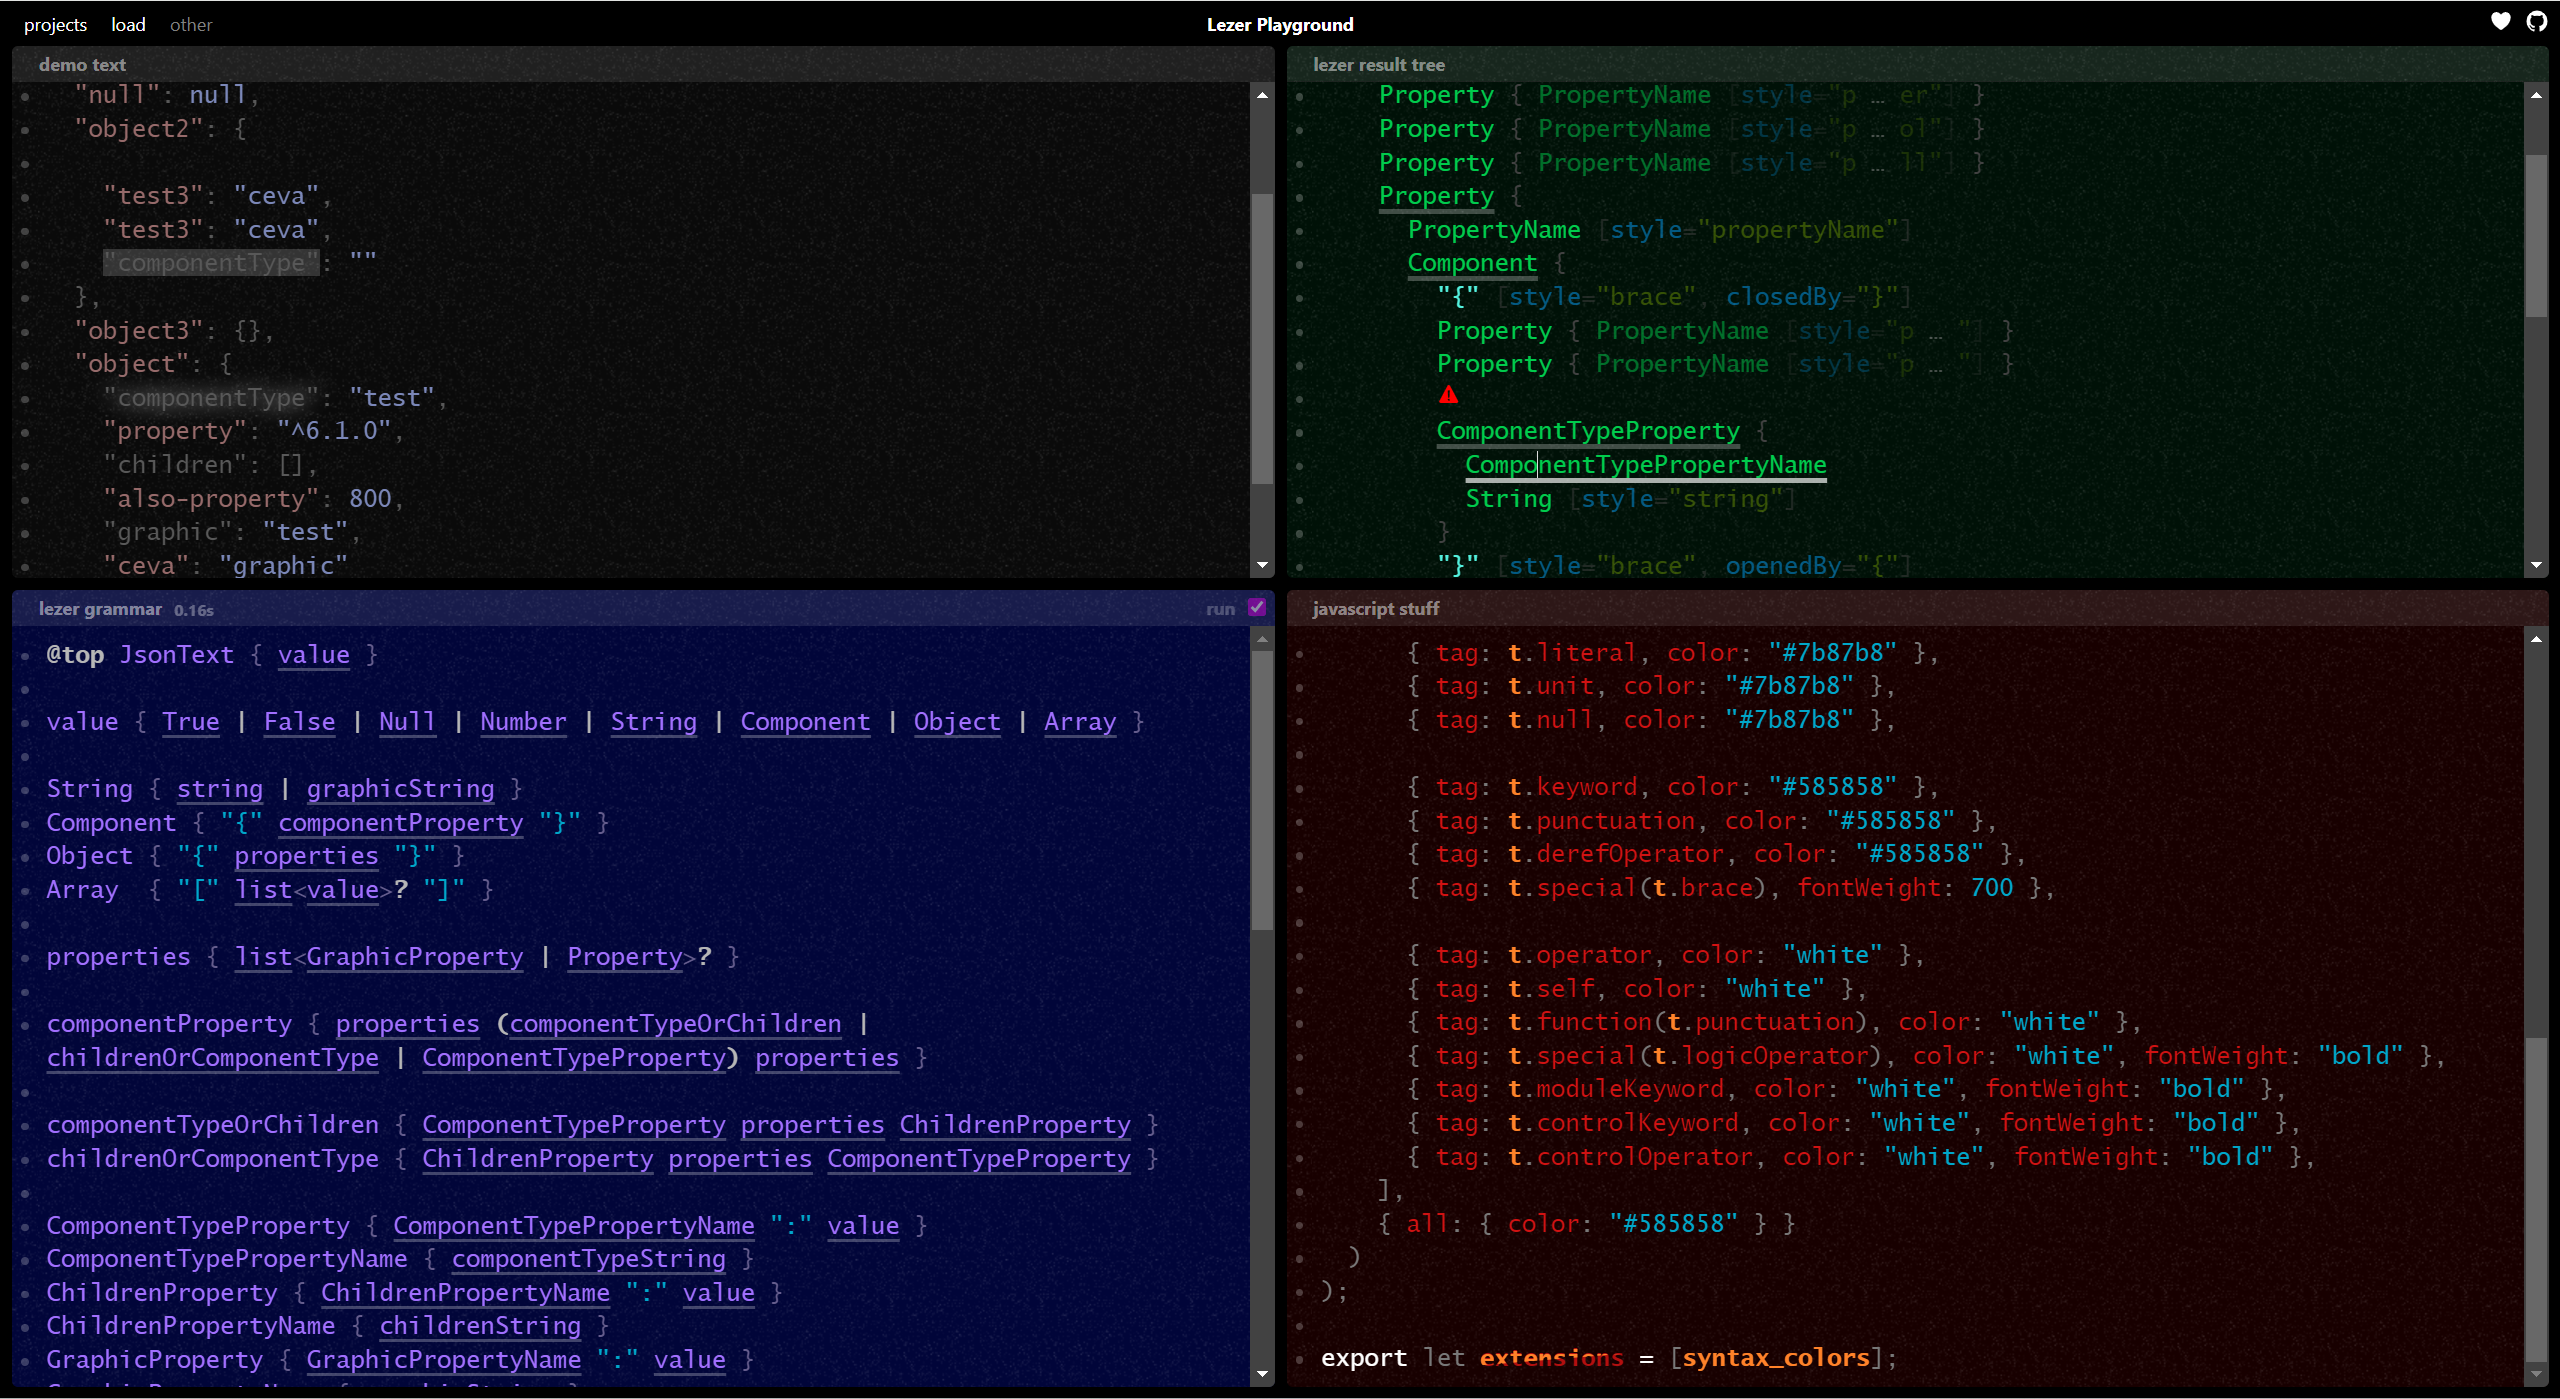
\includegraphics[scale=0.35]{images/lezer-playground.png}
    \caption{Grammar test in the Lezer playground \cite{lezer-playground}}
    \label{fig:lezer-playground}
\end{figure}

\noindent The previously obtained parser is used to create a language extension for the CodeMirror editor. This is done inside the \textbf{json-course-language.ts} file, located inside the \hl{@/modules/courses/utils} folder. Now that the parser has been encapsulated in a \textbf{LanguageSupport} object, it can be used directly in the extensions list.

\subsection{Linting}

\noindent Since Components are defined with a configuration that contains parameters information, those can be used to offer personalized linting messages. Warnings are provided when a component is missing a mandatory parameter, or when a parameter is not of the correct type. The linting messages are displayed in the gutter of the editor. 
\\\\
\noindent Without a custom syntax tree, to identify the type of the component and its children, the linter would need to parse the JSON content and analyze it. This would be a very heavy operation, especially for large JSON files. To avoid this, the custom syntax tree is used, which is generated by the Lezer parser. The linter can now easily identify the type of the component and its children, by using search based on the custom properties added to the JSON grammar.
\\\\
Although the current grammar is not very complex and doesn't add a lot of optimization, it is a good start for future improvements. The linter can be extended to offer more personalized messages or there could be multiple grammars that map different languages to the same syntax tree, which would allow the linter to be used for multiple languages.
\\\\
\noindent If linter errors are identified, the editor will display a red dot in the gutter, and the line with the error will be highlighted. Hovering over the red dot will display the error message (see Figure \ref{fig:json-editor-linter-error}). While errors are present, the content of the editor will not replace the JSON content of the course, as the user might not be aware of the error. The user will be able to save the content only after the errors are fixed.

\begin{figure}[h]
    \centering
    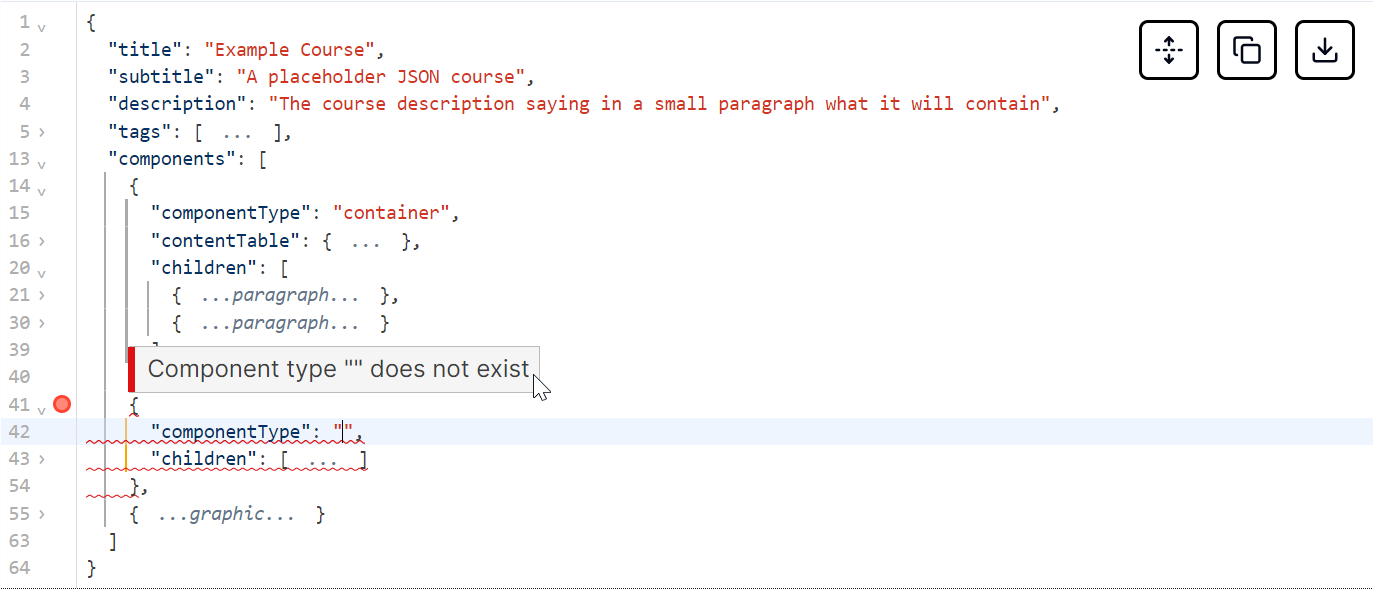
\includegraphics[scale=0.62]{images/json-editor-linter-error.png}
    \caption{JSON Editor - Linter Error Example}
    \label{fig:json-editor-linter-error}
\end{figure}

\subsection{Autocomplete}

\noindent There are two types of autocompletion that are implemented in the JSON editor. The first one is the autocompletion of the components (see Figure \ref{fig:json-editor-autocomplete-components}). When typing a componentType inside the components/children property, a list of components will be displayed. The second one is the autocompletion of the parameters (see Figure \ref{fig:json-editor-autocomplete-fields}). When typing a parameter inside a component, a list of parameters will be displayed. The parameters are filtered based on the componentType that is being typed.
\\\\
\noindent After a suggestion offered by the CodeMirror editor is selected from the list of suggestions generated by the custom extensions \textbf{json-autocomplete-components.ts} and \textbf{json-autocomplete-parameters.ts}, it will be inserted inside the editor at the cursor position. The code snippet that gets inserted might contain placeholders for values, which can be navigated through by pressing the tab key. The placeholders are replaced with the actual value when the user types something.

\begin{figure}[h]
    \centering
    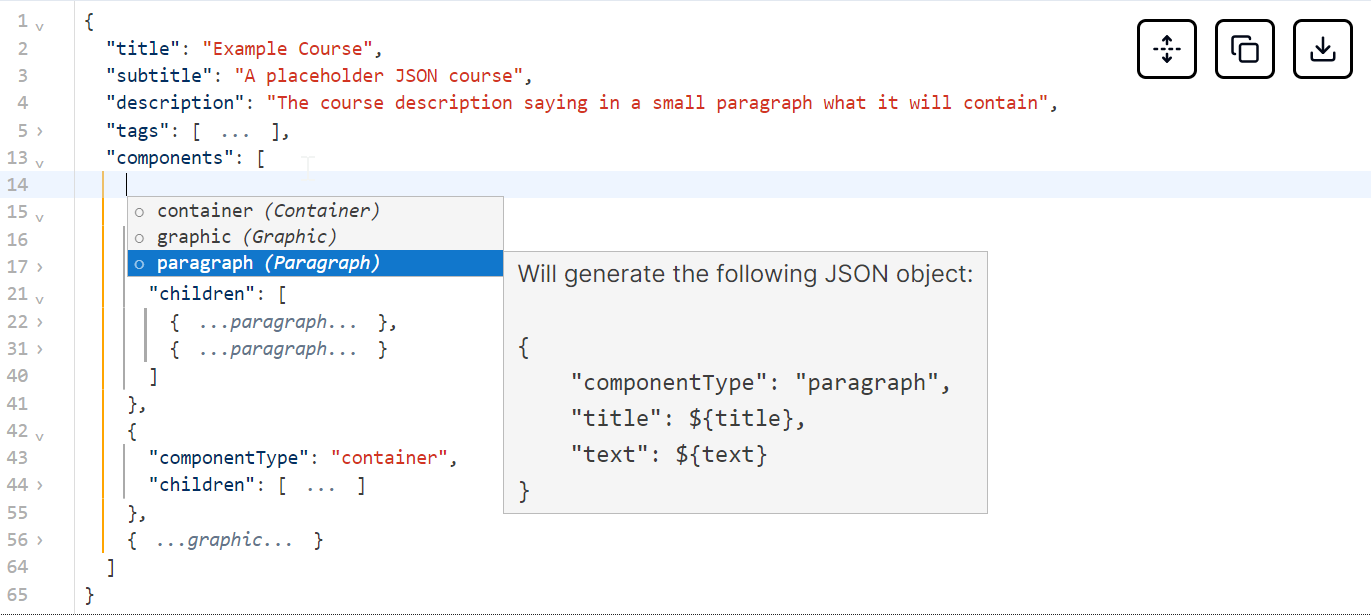
\includegraphics[scale=0.65]{images/json-editor-autocomplete-components.png}
    \caption{JSON Editor - Components Autocomplete Example}
    \label{fig:json-editor-autocomplete-components}
\end{figure}

\begin{figure}[hbt!]
    \centering
    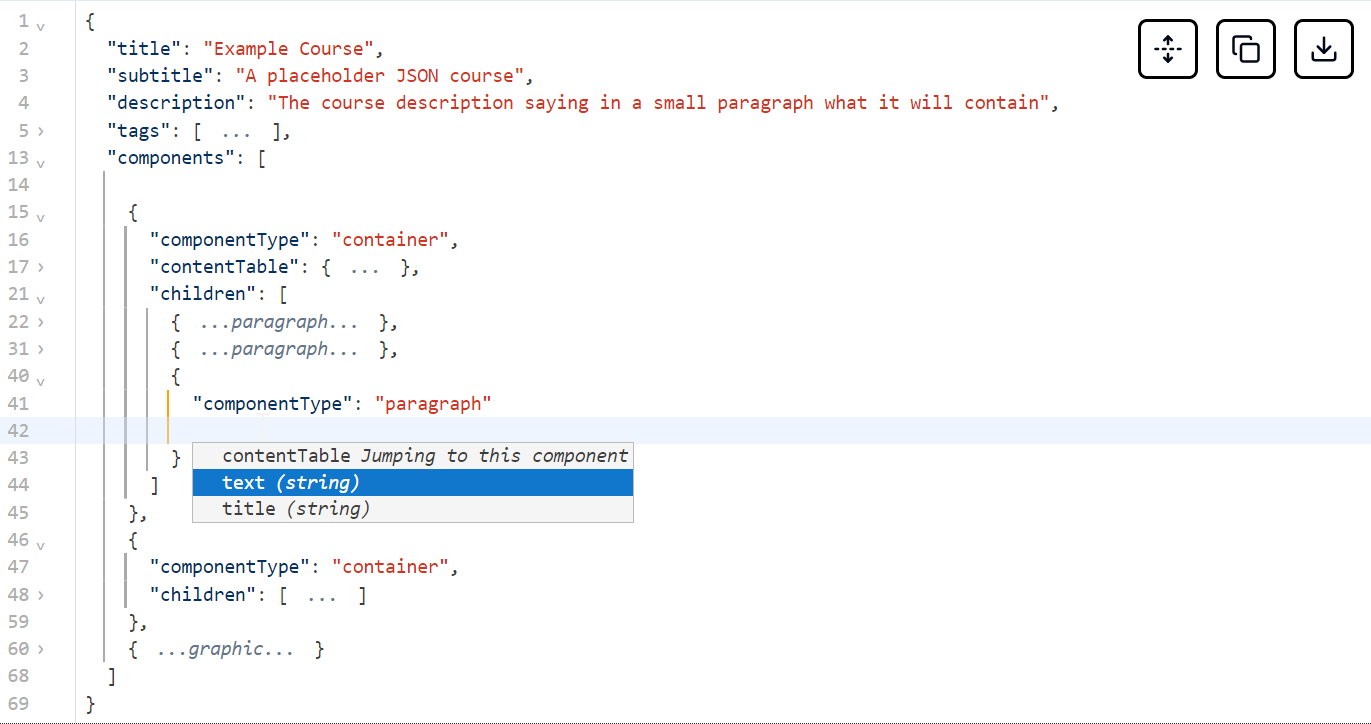
\includegraphics[scale=0.65]{images/json-editor-autocomplete-fields.png}
    \caption{JSON Editor - Properties Autocomplete Example}
    \label{fig:json-editor-autocomplete-fields}
\end{figure}

\noindent Autocomplete snippets can even get more dynamic, by providing code snippets that are always different when the suggestion is accepted. An example of this, is generating the \textbf{contentTable} property which will generate a unique UUID for each entry. The contentTable needs to have an unique id, as the table of contents has a \textbf{goto feature} that allows the user to navigate to the component that is clicked. The required UUIDs are generated by the \texttt{uuid} npm package, which is a simple and efficient way to generate unique identifiers.
\\\\
\noindent This is by far one of the most helpful features of the editor, as it can guide the user through the creation of a course, offering suggestions for components and parameters. The user can also learn about the components and their parameters by reading the suggestions. The autocomplete feature is also a good way to avoid typos, as the user can select the correct component or parameter from the list of suggestions.

\subsection{AutoRepair JSON}

\begin{figure}[h]
    \centering
    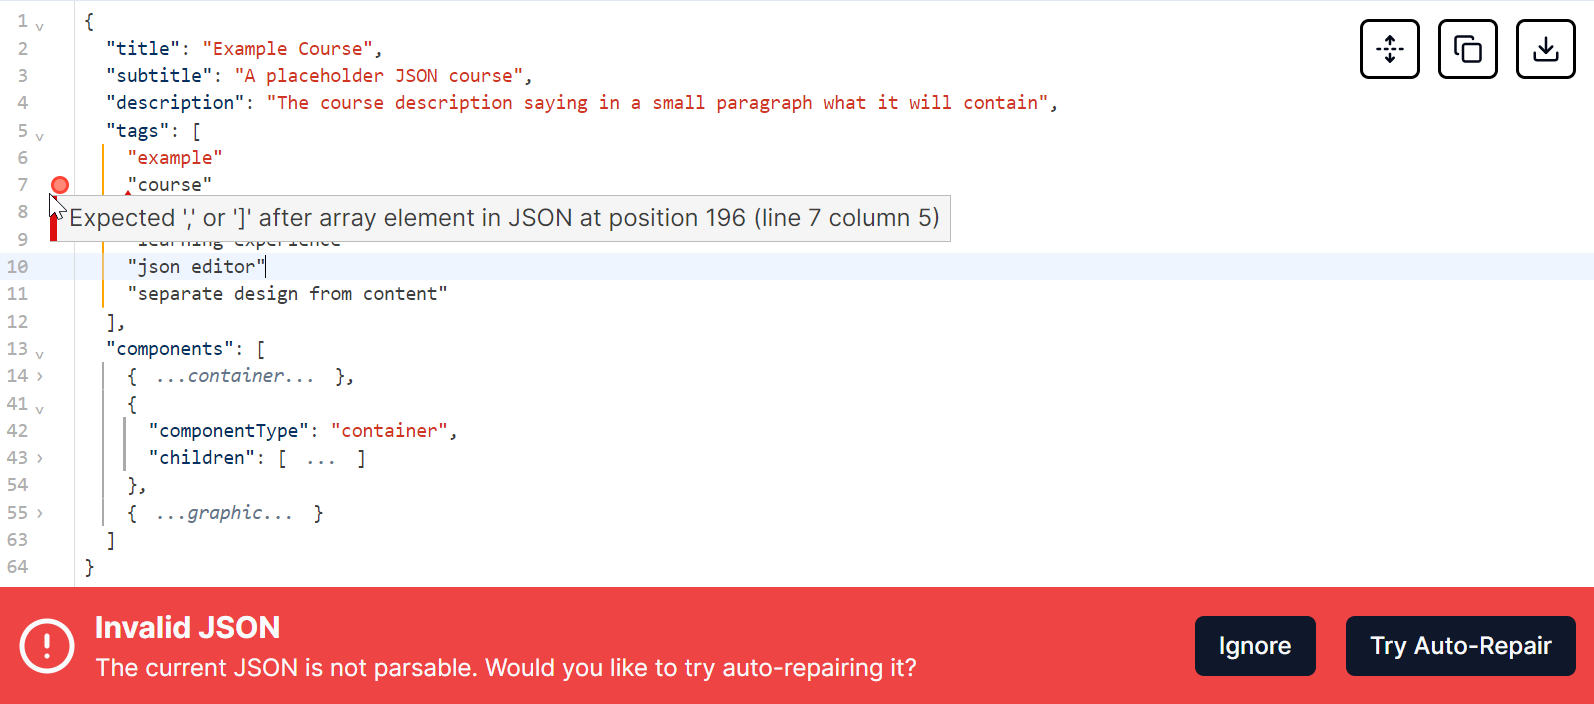
\includegraphics[scale=0.55]{images/json-editor-autorepair.png}
    \caption{JSON Editor - AutoRepair Prompt}
    \label{fig:json-editor-autorepair}
\end{figure}

\begin{figure}[h]
    \centering
    
\includegraphics[scale=1]{images/json-editor-autorepair-success.png}
    \caption{JSON Editor - AutoRepair Success Toast}
    \label{fig:json-editor-autorepair-success}
\end{figure}

\begin{figure}[hbt!]
    \centering
    
\includegraphics[scale=1]{images/json-editor-autorepair-error.png}
    \caption{JSON Editor - AutoRepair Error Toast}
    \label{fig:json-editor-autorepair-error}
\end{figure}

\noindent When working with JSONs you will often encounter the problem of missing commas, brackets, or quotes. This can be very frustrating, as the JSON will not be valid and the editor will not be able to parse it. To avoid this, the editor is equipped with an \textbf{AutoRepair} feature. The feature is implemented inside the \textbf{json-auto-repair-lint.ts} file, located inside the \hl{@/modules/courses/utils} folder.
\\\\
\noindent Inside the JSON Editor, whenever a JSON parse exception is encountered, one that does not belong to the custom linter, in the bottom of the editor an alert box will be displayed, which gives the user two options (see Figure \ref{fig:json-editor-autorepair}). They can choose to ignore the error, which will make the box disappear until the error changes or is fixed, or they can choose trying to auto-repair it. A \textbf{toast} message with the result of the auto-repair operation will be displayed in the bottom right corner of the screen (see Figures \ref{fig:json-editor-autorepair-success} and \ref{fig:json-editor-autorepair-error}).
\\\\
\noindent For auto-repairing, the \textbf{jsonrepair} npm package is used. It provides a lot of features regarding the JSON, besides handling commas, brackets, and quotes. The package can also handle the removal of comments, trailing commas, and other JSON specific problems. It helps with compatibility, as it also replaces Python and MongoDB specific syntax with the standard JSON syntax.
\\\\
\noindent It is important to keep in mind that the auto-repair feature is not a replacement for the linter. The linter is used to provide personalized messages for the user, while the auto-repair feature is used to quickly fix the JSON so it can be parsed. The linter will still display errors if the JSON is not correctly written, even after the auto-repair operation. There might even be times when the auto-repair operation will not be able to fix the JSON, but the linter will still be able to provide a message for the user.
\\\\
\noindent Its important to check the place of the error after the JSON is auto-repaired, as the auto-repair might decide that instead of adding a quote and a missing comma, it will concatenate the two strings. This is a rare case, but it can happen, and the user should be aware of it. Even if it occurs, it will be obvious in the live preview that the component is not displayed correctly.

\subsection{Live Preview}

\noindent The live preview is a feature that allows the user to see the course as it would be displayed on the web platform. The live preview is displayed in the right side of the editor (see Figure \ref{fig:live-preview-editor}), and it is updated in real-time as the user types.
\\\\
\noindent To make this possible, since usually the two sides (middle and right) are handled separately, a \textbf{React Context} is used to share the JSON content between them. A provider is created inside the \textbf{course-json-provider.tsx} file, located inside the \hl{@/modules/courses/context} folder. The provider is wrapped around the layout of the whole courses section. Of course, the provider should not be used outside the editor, although it is available everywhere in this section. For this reason, the course JSON from inside the provider is cleared when the route changes, using an \textbf{useEffect} that relies on Next.js' \textbf{usePath} hook.

\begin{figure}[h]
    \centering
    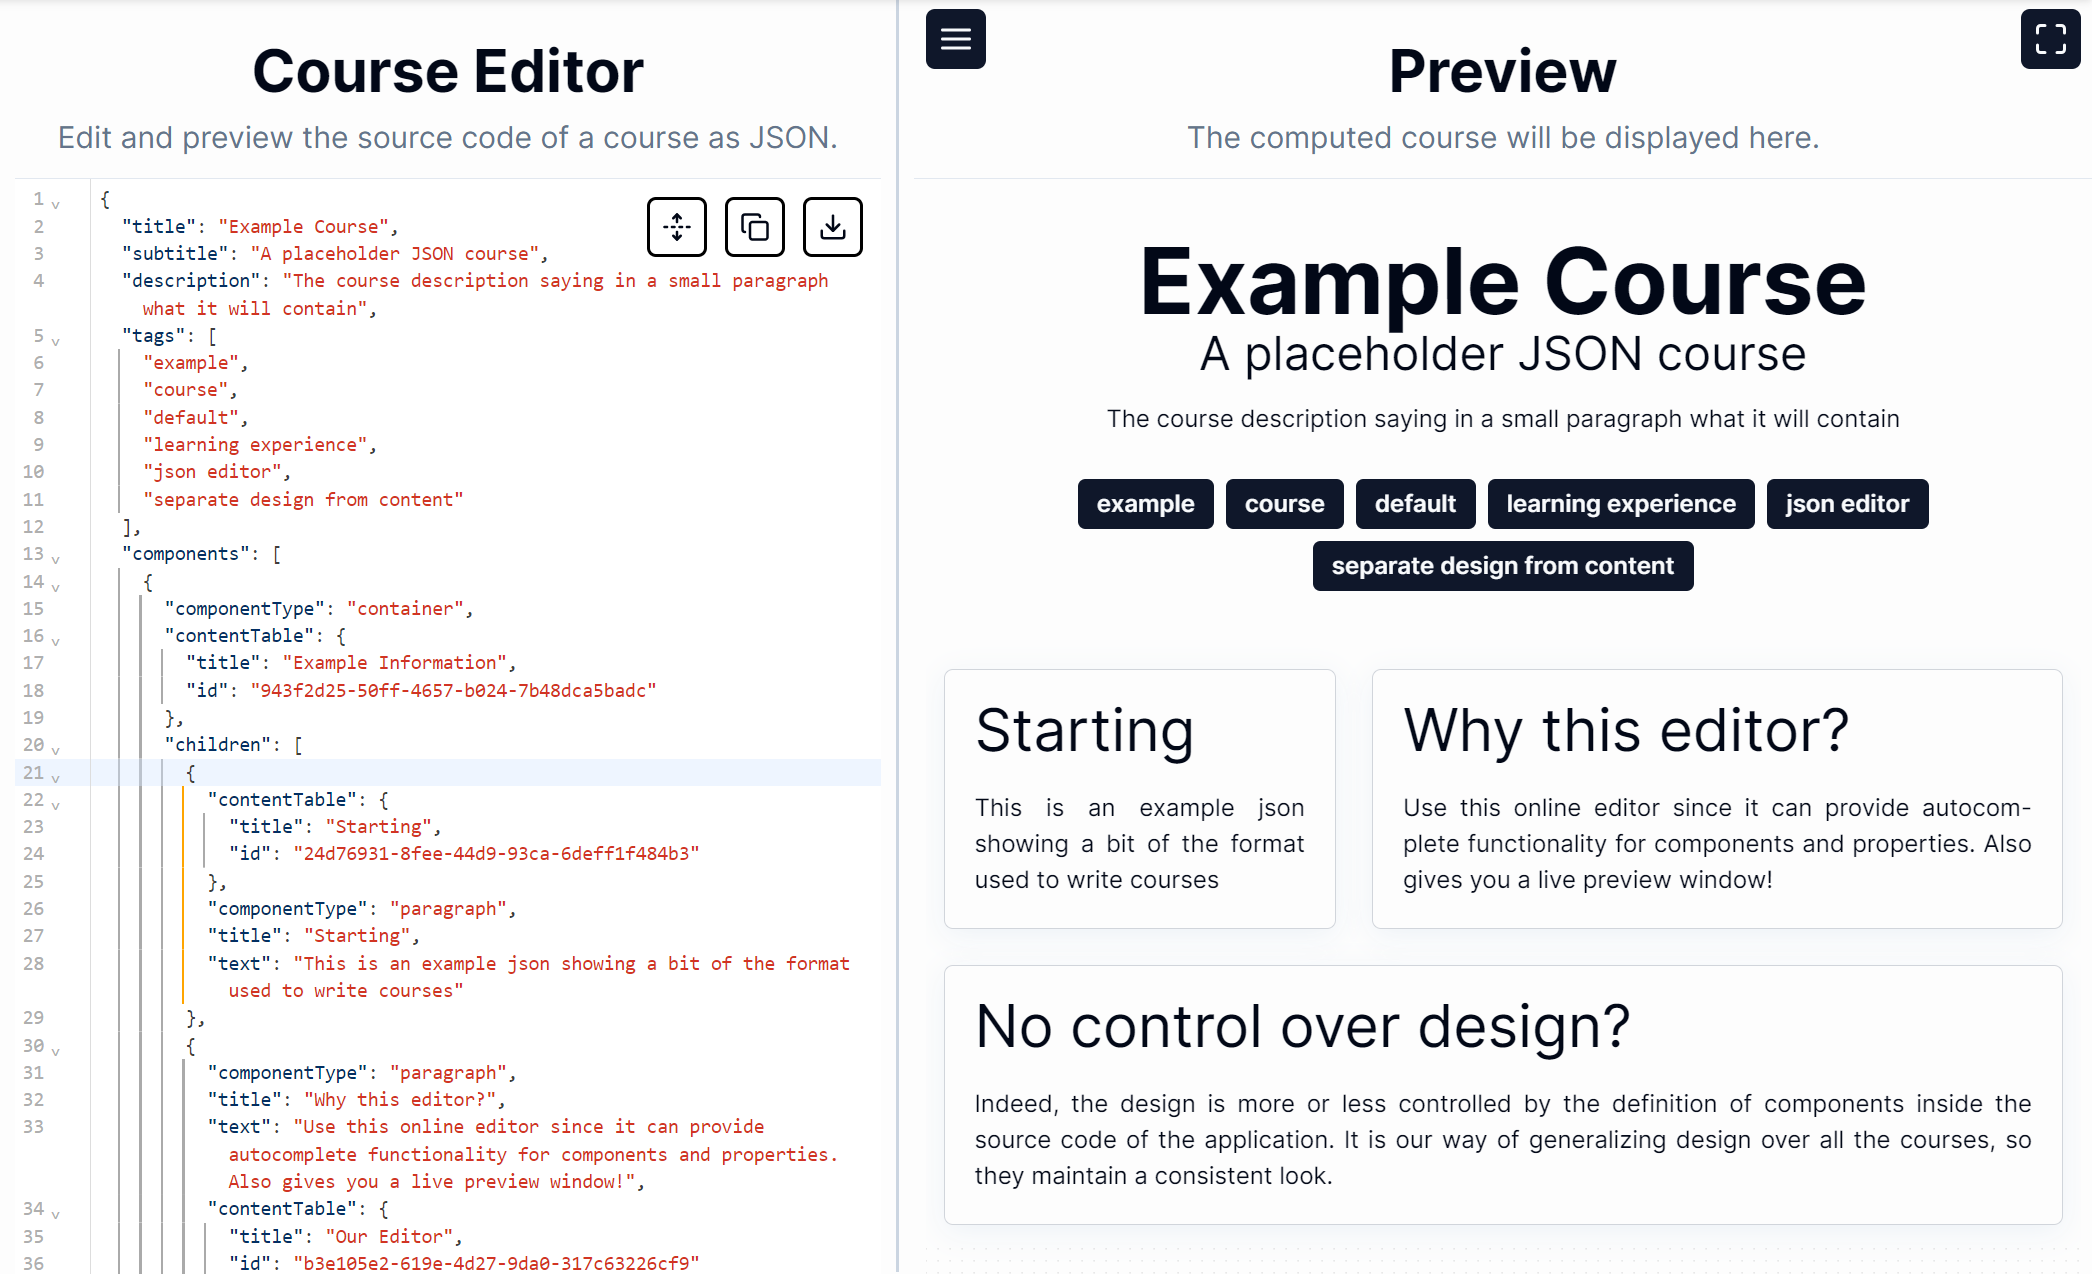
\includegraphics[scale=0.45]{images/live-preview-editor.png}
    \caption{JSON Editor with Live Preview}
    \label{fig:live-preview-editor}
\end{figure}
\newpage
\noindent To facilitate the \textbf{Save changes} option of the editor, the JSON is stored in two variables, initialCourseJSON and inEditCourseJSON. The two JSONs are used to compare the changes made by the user. If the user decides to save the changes, the inEditCourseJSON will be sent to the backend.
\\\\
\noindent To avoid desynchronization, the initialCourseJSON and the inEditCourseJSON need to be updated at the same time, when fetched from the database. For this reason they are both wrapped in the same variable, wholeJSON. To wholeJSON is exposed as courseJSON to the editor, along with three functions, setInitialCourseJSON and setInEditCourseJSON, that are used to update the JSONs, and internally use the setWholeJSON function to update the wholeJSON variable.
\\\\
\noindent Monitoring the inEditCourseJSON, the right side will rerender the live preview whenever the JSON changes. The live preview uses the actual course component, which was designed to allow for dynamic changes, by including error boundaries and having cached components based on the provided JSON.
\\\\
\noindent Since the right side might not be enough to fully visualize the course, in the top right corner a button is added that allows for a bigger display, by opening a dialog that spans over the entire page. Besides that, in the top left corner, a button for previewing the table of contents is added. The table of contents is a list of all the components that are present in the course, and it allows the user to navigate to a specific component by clicking on it. The user might not want to display all components inside the table, so only components annotated with the \textbf{contentTable} property are displayed. Based on their depth level, the components are indented, and the user can easily see the hierarchy of the course.

\section{Graphics/Diagrams}

Information can sometimes be better conveyed through graphics. For this reason, the web platform offers a graphic editor that can be used to create diagrams. Unlike the course editor, this one is not a code editor, but a visual editor (see Figure \ref{fig:graphic-editor}). The graphic editor is used to create graphics that can be used inside the course editor.

\begin{figure}[h]
    \centering
    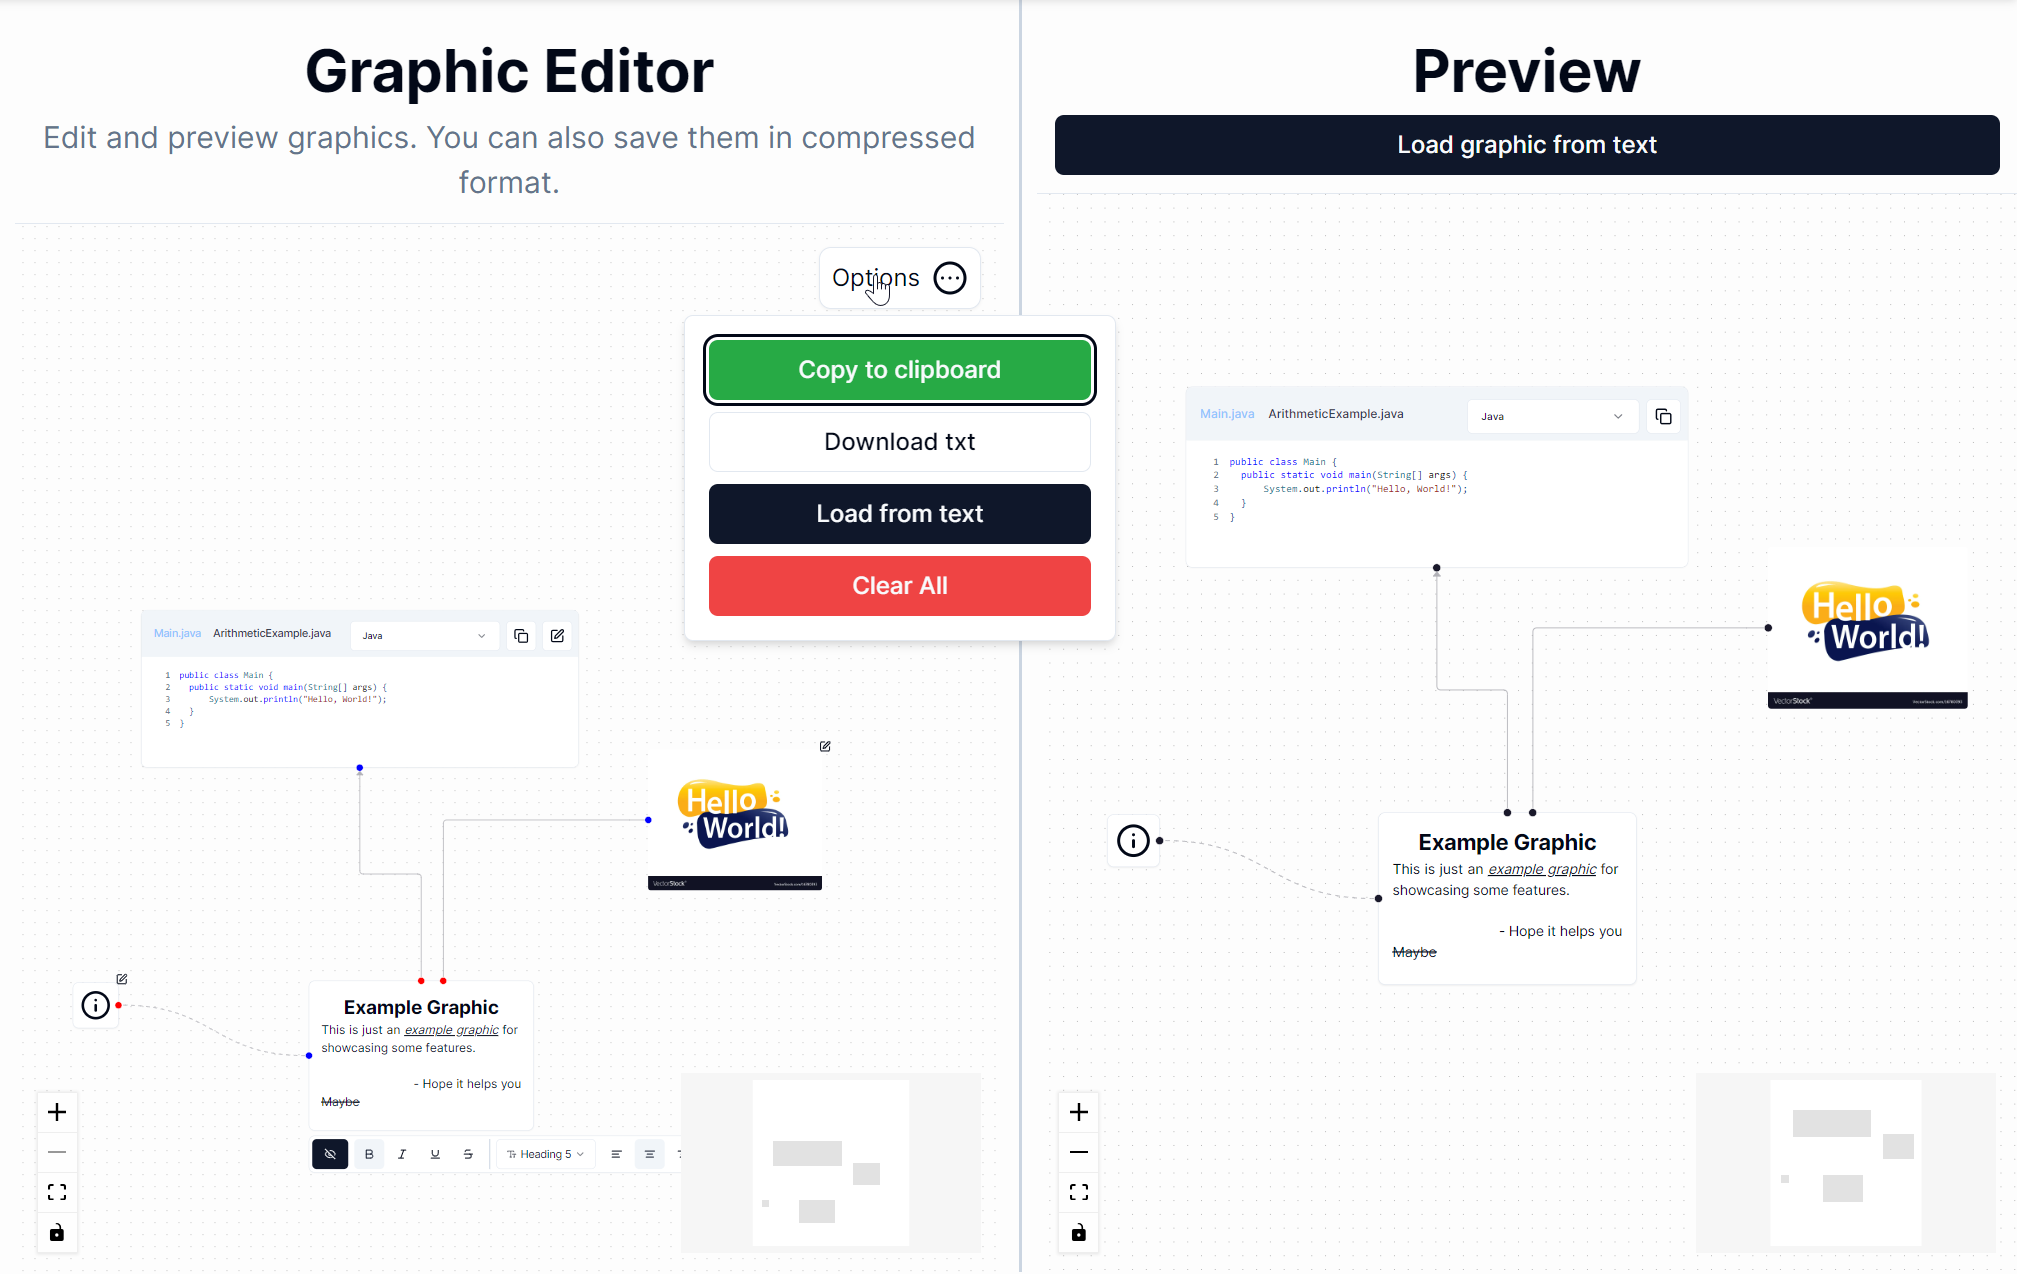
\includegraphics[scale=0.45]{images/graphic-editor.png}
    \caption{Graphic editor with example graphic}
    \label{fig:graphic-editor}
\end{figure}

\subsection{Diagrams Library}

\noindent For the graphics, the \textbf{ReactFlow} library \cite{reactflow} was chosen. This library offers a component with a graph like structure, that can be used to create diagrams. The library is very flexible, and it can be used to create a wide variety of diagrams, from flowcharts to mind maps.
\\\\\newpage
\noindent Elements are added to the graph via nodes and edges. Both the nodes and the edges offer various customization options, ReactFlow allowing developers to even create their own components for them. Besides that, the canvas itself is very customizable, allowing for zooming, panning, and even the creation of custom background elements. It also allows for the personalization of the actions menu.
\\\\
\noindent Besides the design customization, ReactFlow also offers dynamic interaction with the elements from the graph. The elements can be dragged, resized and connected. The canvas itself can be dynamically resized without causing elements inconsistencies.
\\\\
\noindent The state of the graph can also be stored in an external JSON, which can be used to recreate the graph at a later time. This is very useful for the web platform, as the graphics created by the user can be stored in the course JSON, and displayed in the course view. The JSON can also be used to recreate the graphic in the graphic editor, in case the user wants to make changes to it.
\\\\
\noindent The learning curve of this library also proved to be very low, as the documentation is very well written and the examples are very helpful.

\subsection{Nodes}

\noindent At the time at which this thesis was written, there are four types of nodes: image, code, rich text and information. More nodes might be added in the future, but the current ones are enough to cover a wide range of use cases. Besides the type of nodes, there exists two copies of each node, one for the graphic editor and one for the display inside the course. The nodes are stored in the \hl{@/modules/courses/components/graphic/nodes} folder.

\begin{figure}[h]
    \centering
    \begin{minipage}{0.45\textwidth}
        \centering
        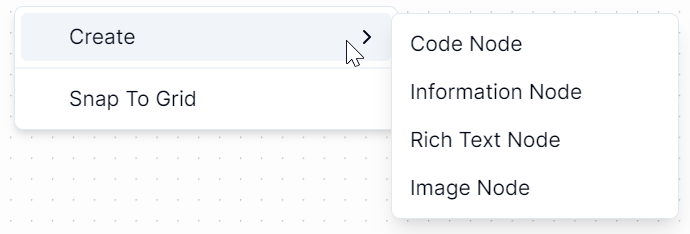
\includegraphics[width=1\linewidth]{images/canvas-context-menu.png}
    \end{minipage}%
    \hspace{0.1\textwidth}% 
    \begin{minipage}{0.45\textwidth}
        \centering
        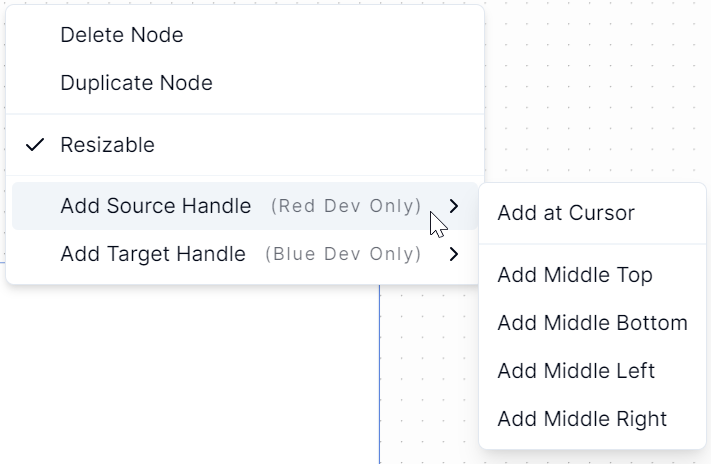
\includegraphics[width=1\linewidth]{images/node-context-menu.png}
    \end{minipage}
    \caption{Canvas and Node Context Menus}
    \label{fig:context-menus}
\end{figure}

\noindent For taking actions regarding nodes, the graphic editor relies on two context menus (Figure \ref{fig:context-menus}). The first one is the node context menu, which is displayed when right clicking on a node. The second one is the canvas context menu, which is displayed when right clicking on the canvas. The context menus are used to offer actions that can be taken on the nodes, such as creating a node at a given position, delete a selected one, or duplicate it. The context menus are stored in the \hl{@/modules/courses/components/graphic/context-menu} folder.
\\\\
\noindent The \textbf{rich text node} is a text editor itself, that gives you a bit more customization than just a textarea. For this, an equivalent for CodeMirror exists, named \textbf{ProseMirror}, which is a toolkit for building rich text WYSIWYG editors. To expand on the power of ProseMirror, a headless wrapper around it is used, to offer more out of the box extensions. The wrapper is \textbf{TipTap} \cite{tiptap}, that is also compatible with React. The editor is used to offer more customization options for the text, such as bold, italic, underline, lists, text alignment and so on. While very customizable, the functionalities of the editor are limited, as to focus on a consistent design, without too many overwhelming options.

\begin{figure}[hbt!]
    \centering
    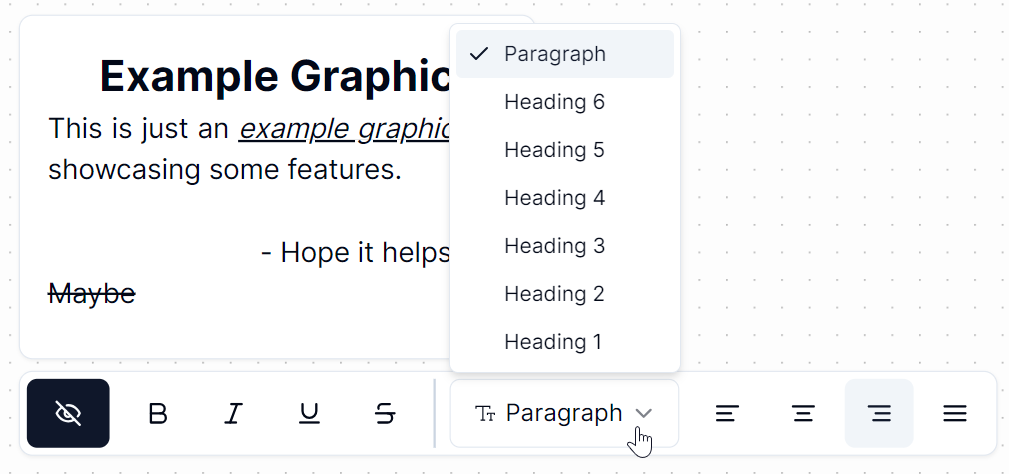
\includegraphics[scale=0.62]{images/rich-text-node.png}
    \caption{Rich text node with editor}
    \label{fig:rich-text-node}
\end{figure}

\noindent The \textbf{image node} is used to display images inside the graphic. Currently, images can only be added via a URL, but in the future, the user might be able to upload images from their computer. Since the node can be resized, an extra option is offered, to keep the aspect ratio of the image (see Figure \ref{fig:image-node-editor}).

\begin{figure}[hbt!]
    \centering
    \begin{minipage}{0.45\textwidth}
        \centering
        
\includegraphics[width=0.72\linewidth]{images/image-node.png}
        \caption{Initial Image Node}
        \label{fig:image-node}
    \end{minipage}%
    \hspace{0.1\textwidth}% 
    \begin{minipage}{0.45\textwidth}
        \centering
        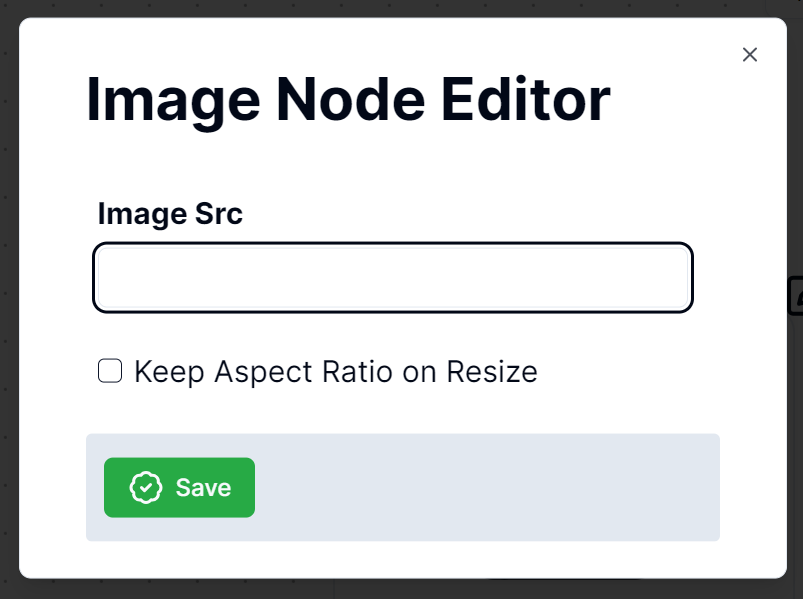
\includegraphics[width=1\linewidth]{images/image-node-editor.png}
        \caption{Image Node Editor}
        \label{fig:image-node-editor}
    \end{minipage}
\end{figure}

\noindent The \textbf{information node} is a small box with an information icon, that when hovered over, displays a tooltip with the information. This node is used to display information that is not directly visible in the graphic, as to not overwhelm the user. From its editor you can change the inner information and the side the tooltip should appear on.

\begin{figure}[hbt!]
    \centering
    \begin{minipage}{0.45\textwidth}
        \centering
        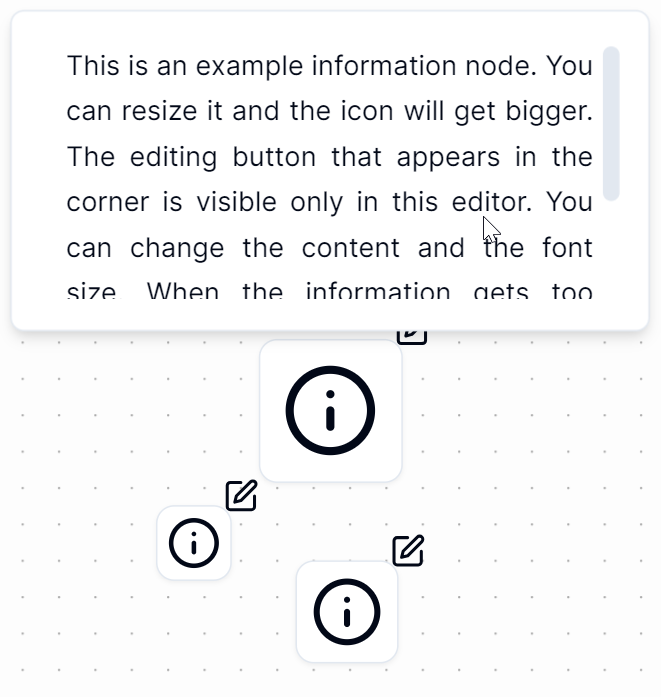
\includegraphics[width=1\linewidth]{images/information-node.png}
        \caption{Information Nodes}
        \label{fig:information-node}
    \end{minipage}%
    \hspace{0.1\textwidth}% 
    \begin{minipage}{0.45\textwidth}
        \centering
        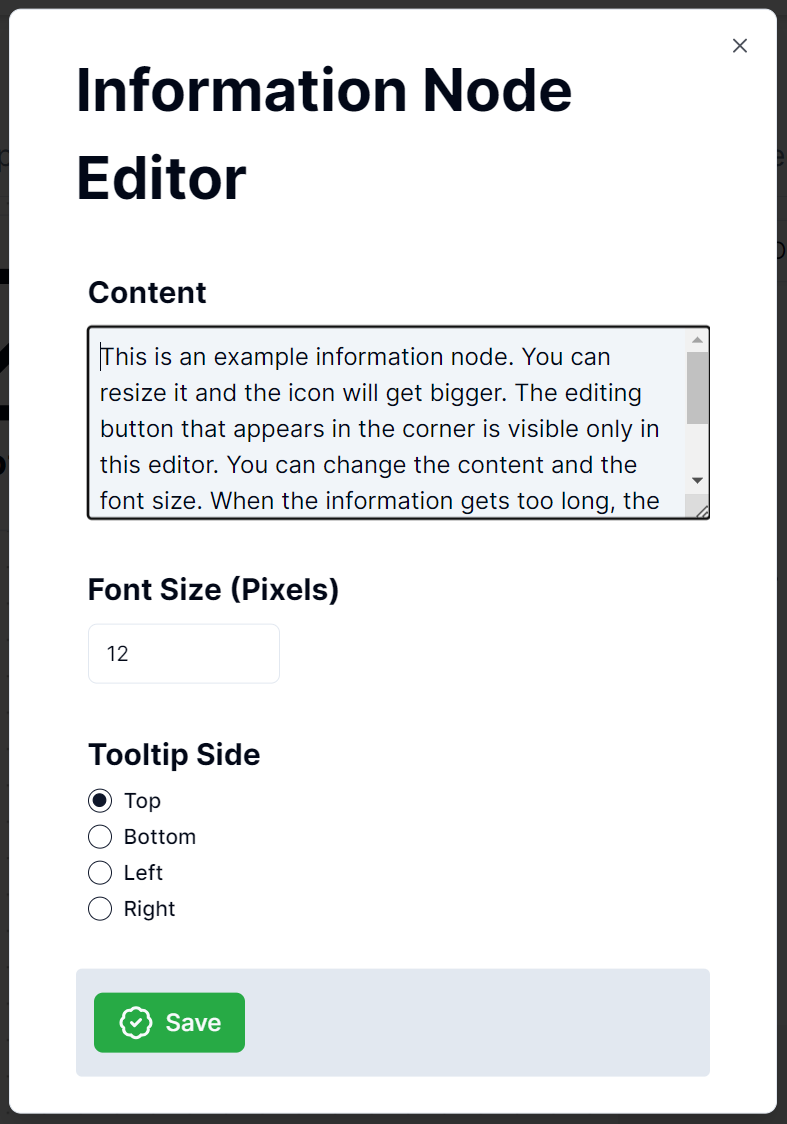
\includegraphics[width=1\linewidth]{images/information-node-editor.png}
        \caption{Information Node Editor}
        \label{fig:information-node-editor}
    \end{minipage}
\end{figure}
\noindent \\
\noindent The \textbf{code box node} is used to display code inside the graphic. For the highlight of the code, Prism.js \cite{prismjs} is used, which is a lightweight, extensible syntax highlighter. Prism.js is implemented in the web platform through a React wrapper, provided by the \textbf{prism-react-renderer} npm package. The code box node is used to display code snippets that are relevant to the graphic. The code box is designed to allow for multiple code snippets inside the display, either by having multiple files inside the code box, or by having a dropdown button that lets you change the language of the code snippet. Besides that, the code box contains a copy button, that will copy to clipboard the code from the active file. The editor of the code box is also very complex, and it relies on a JSON editor is as well. To avoid having a very long JSON, for the actual code snippets placeholders are used. You can create multiple snippets inside the editor, and then reference them inside the JSON configuration. The configuration itself is for specifying the languages the code box supports and the files that should be displayed.

\begin{figure}[hbt!]
    \centering
    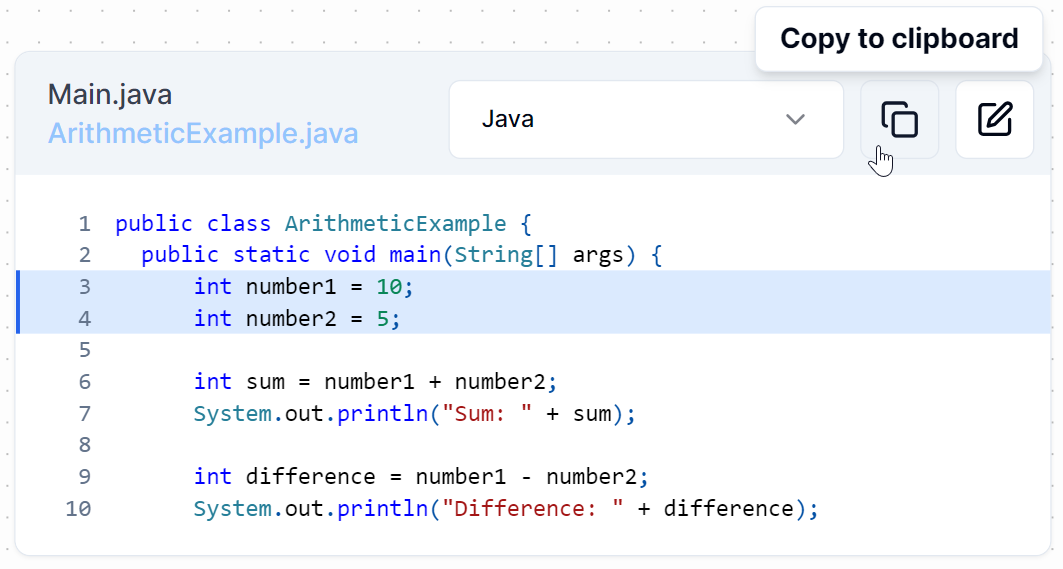
\includegraphics[scale=0.65]{images/code-node.png}
    \caption{Code node with example code}
    \label{fig:code-node}
\end{figure}
\newpage
\noindent If in the future there will be a need for more nodes, the graphic editor can be extended without affecting the current ones. If some of the current nodes will change or be deleted, the graphic's JSON like structure allows for simply ignoring the nodes that are not recognized.

\subsection{Edges}

\noindent By edges, it should be understood the lines between the nodes. The edges are used to show a connection between two nodes. They also have different customization options, from their display to the handles of the node they are connected with. The edges are stored in the \hl{@/modules/courses/components/graphic/edges} folder.
\\\\
\noindent The edges also have a context menu, that is displayed when right-clicking on an edge (see Figure \ref{fig:edges-context-menu}). The context menu is used to offer actions that can be taken on the edges, such as changing the line style, if it should be dashed or not, if it should have a marker at the start/end. The context menu is stored in the \hl{@/modules/courses/components/graphic/context-menu} folder.
\\\\
\noindent Edges can be straight, bezier, step or smoothstep (see Figure \ref{fig:edges}). The \textbf{straight edge} is the most basic one, connecting two nodes with a straight line. The \textbf{bezier edge} is a curved line, that connects two nodes. The \textbf{step edge} is a line that connects two nodes with a series of horizontal and vertical lines. The \textbf{smoothstep edge} is a line that connects two nodes with multiple straight lines, that are smoothed out at the corners. The markers that can be placed at the start and the end of the edges can be open/closed arrows or circles. They are optional, and can be added or removed from the context menu. When an edge becomes dashed, it will also have a flowing animation, from start to end.

\begin{figure}[hbt!]
    \centering
    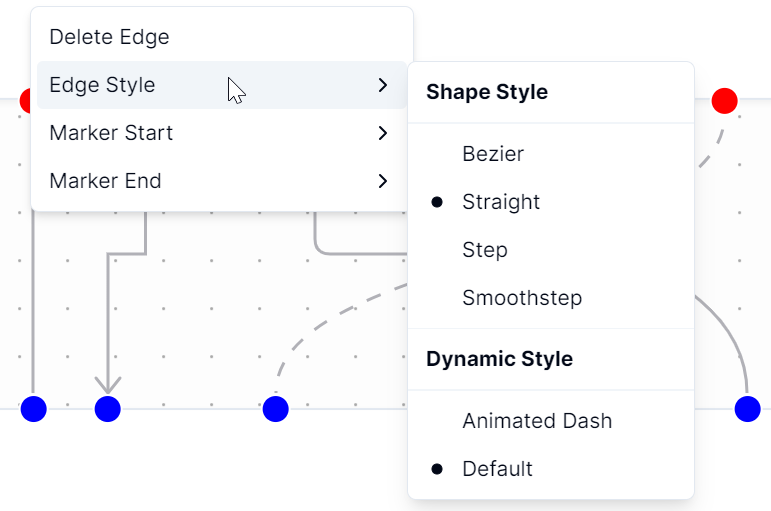
\includegraphics[scale=0.75]{images/edges-context-menu.png}
    \caption{Edge context menu}
    \label{fig:edges-context-menu}
\end{figure}

\begin{figure}[hbt!]
    \centering
    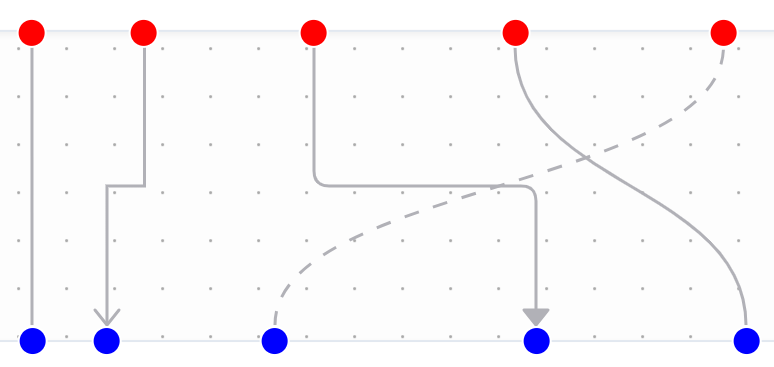
\includegraphics[scale=0.75]{images/edges.png}
    \caption{Edge types}
    \label{fig:edges}
\end{figure}

\noindent More customization can be added to the edges in the future, such as custom colors, thickness, or even animations. The current customization options are enough to cover a wide range of use cases, and they are very easy to use.
\\\\
\noindent The edges are connected to a node at specific points called handlers. The customization of these handles allows for easier understanding of the connections, as they can be added in dynamic positions of the node, while with fixed positions you might end up with overlapping lines. You can still add them in cardinal positions, middle right, middle left, middle top, middle button, but they can also be added relative to the position of the cursor.

\subsection{Graphic Object}

\noindent To avoid having to store graphics as JSON entities in the database, and giving them a tighter integration inside the course JSON a solution had to be found to make the graphic object a much more compact entity.
\\\\
\noindent To achieve this, the first thought was to store the graphic as a base64 string. This would have been a good solution, as the graphic would be stored as a string, and it would be easy to display it inside the course view. The problem with this solution is that the graphic would be very long, and it would take a lot of space.
\\\\
\noindent Since a base64 string is more compact than the raw JSON stringified, this approach was kept, but the source it is applied on had to change. For this reason, a compression algorithm on the stringified JSON, or on the bytes of the JSON themselves, could be applied to improve the memory usage. The graphic structure could for sure benefit of compression, as the JSON structure is very repetitive, and the same properties are used multiple times.
\\\\
\noindent In the end, the \textbf{JSONCrush} library \cite{jsoncrush} was used. It compresses JSON similar to the \textbf{zip} algorithm. Comparing the base64 string of the stringified JSON to the crushed JSON that the library outputs, it can be seen that the crushed JSON is much shorter, especially for more complex graphics.
\\\\
\noindent The graphic object ends up being a portable base64 string, obtained by stringifying the JSON, crushing it with the library, and finally converting it. When displaying the graphic, either in the editor or the course component, the process is reversed and the obtained JSON is processed by ReactFlow.

\section{Security}

Inside a web platform, we can't rely on the user to always have good intentions, so security for private data can't be implemented inside the frontend. For this reason, any private logic as session handling or database access is done either directly in the Spring Boot backend, or through the backend of the NextJS, the middleware. The frontend is only responsible for the visual representation of the data, and the user interaction with it.

\subsection{NextAuth Configuration}

\noindent The web platform uses \textbf{NextAuth} \cite{nextauth} for authentication. I opted for an open source solution that is well maintained and has a lot of features. NextAuth is a complete authentication solution for Next.js applications. It is easy to use, and it offers a lot of providers, such as Google, Facebook, Twitter, GitHub, and many more.
\newpage
\noindent In this web platform, three files are used for setting up NextAuth. The \textbf{route.ts} file, located inside the \hl{@/app/(users)/api/auth/[...nextauth]} folder, is used to catch all routes handled by nextauth. The \textbf{auth.config.ts} file which is responsible for configuration of the providers and adding callbacks, that is located inside the \hl{@/modules/users/next\_auth} folder. The \textbf{nextauth.d.ts} file, located at the root of the frontend project, is used to declare the types of the session object.
\\\\
\noindent The \textbf{route.tsx} is the entry point for NextAuth. It uses the configuration options defined in \textbf{auth.config.ts} to create a handler, that is exported using the GET and POST methods. Inside the \textbf{auth.config.ts} file, various options for NextAuth are declared. Firstly, the default login, logout and error pages are overridden with custom implemented routes. The \textbf{providers} array is used to declare the oauth2 sources that are used for authentication. The \textbf{callbacks} object is used to declare the callbacks that are used for the authentication process. The signIn, jwt and session callbacks are added here, to help process the user data. The \textbf{events} object is used to declare a signOut event, that will also signal the action to the backend.
\\\\
\noindent The \textbf{nextauth.d.ts} file is used to extend the types of the session and token objects. A user interface is declared that adds authorities and backend tokens to use inside the session object. The jwt object also receives this user.
\\\\
\noindent Although not a file with the express purpose of handling NextAuth, the \textbf{middleware.ts} file also uses a middleware object provided by NextAuth. The \textbf{withAuth} middleware is used to protect routes that require authentication. The middleware is used to check if the user is authenticated, and if not, redirect them to the login page.
\\\\
\noindent \textbf{Attention!} It is important to note that the Next's middleware can only intercept requests made between the client and the backend of the NextJS project! If requests to the Spring Boot backend are made directly inside the client, the middleware will not be able to intercept them.

\subsection{OAuth2}

\noindent To avoid the storage of passwords, the web platform uses OAuth2 for authentication. The connection to the third party providers is done through the NextAuth library. The user can choose to authenticate with Discord and GitHub. To connect to these providers, OAuth2 applications have been set up on the respective platforms. The client ID and client secret are stored in the environment variables of the NextJS backend.
\\\\
The access token obtained from the provider is used to further authenticate the user with the Spring Boot authorization server. The access token is sent to the backend, where it is validated and used to create a JWT token. The JWT token is then sent back to the frontend, and stored inside the session object. Two tokens are used, an access token that gives the user access to the resources, and a refresh token that is used to obtain a new access token when the old one expires.
\\\\
\noindent The custom login page, which contains the login card displayed in Figure \ref{fig:login-card}, uses the \textbf{signIn} method provided by NextAuth to initiate the OAuth2 flow with the specified provider. The method accepts two parameters, the name of the provider and the options. Only a callbackUrl is provided as an option, to redirect the user back to the login page after the authentication process is done. The \textbf{signIn} method is called when the user clicks on the login button of the provider.
\\\\
\noindent In the future, more providers can be added, such as Google, Facebook, Twitter, or even custom providers. The process is simple, as the NextAuth library offers a lot of providers, and the setup is easy.

\begin{figure}[hbt!]
    \centering
    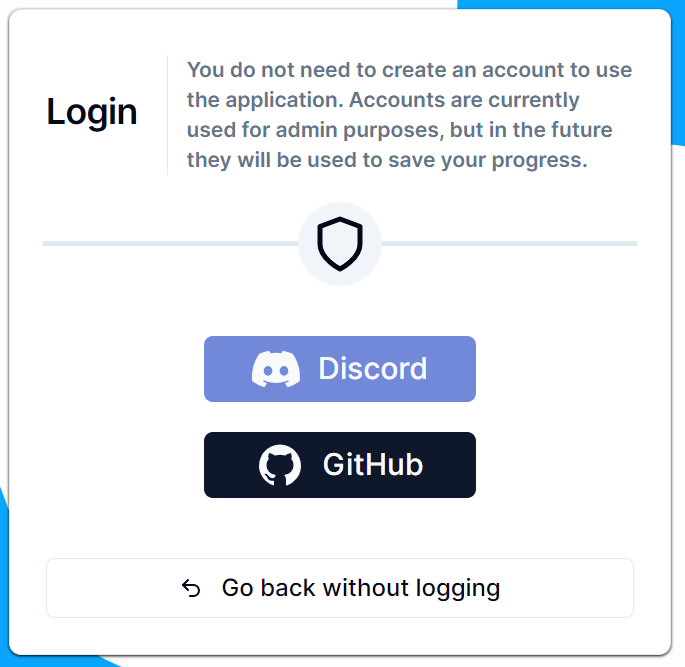
\includegraphics[scale=0.9]{images/login-card.png}
    \caption{Custom Login Card}
    \label{fig:login-card}
\end{figure}


\subsection{User Sessions}

\noindent The user session is stored inside the session object, which is provided by NextAuth. By default, the session object provides data such as email, username and so on. In the modified version used in this web platform, the session holds the user id, their authorities and access and refresh tokens that are used to authenticate the user with the backend.
\\\\
\noindent A global provider, \textbf{SessionEnsure} is used to monitor the session, forcefully signing out the user if the Spring Boot backend session is invalidated. In the context of JWTs, that would mean when the refresh token expires or is marked as invalid. To refresh the access token, two mechanics are employed. Firstly, the jwt callback in NextAuth's configuration is used to refresh the access token whenever it expires. Secondly, in the \textbf{SWR config}, a fetcher that handles onError events is used to refresh the access token whenever a 401 error is encountered.
\chapter{Web Platform Flows}

The previous chapters explain the logic behind the components of the web platform. In this chapter, some of the web platform's flows are explained, either from the user's perspective or from the system's perspective. Some flows presented below are subject to change as the application evolves.

\section{Reading courses}

\begin{figure}[h]
    \centering
    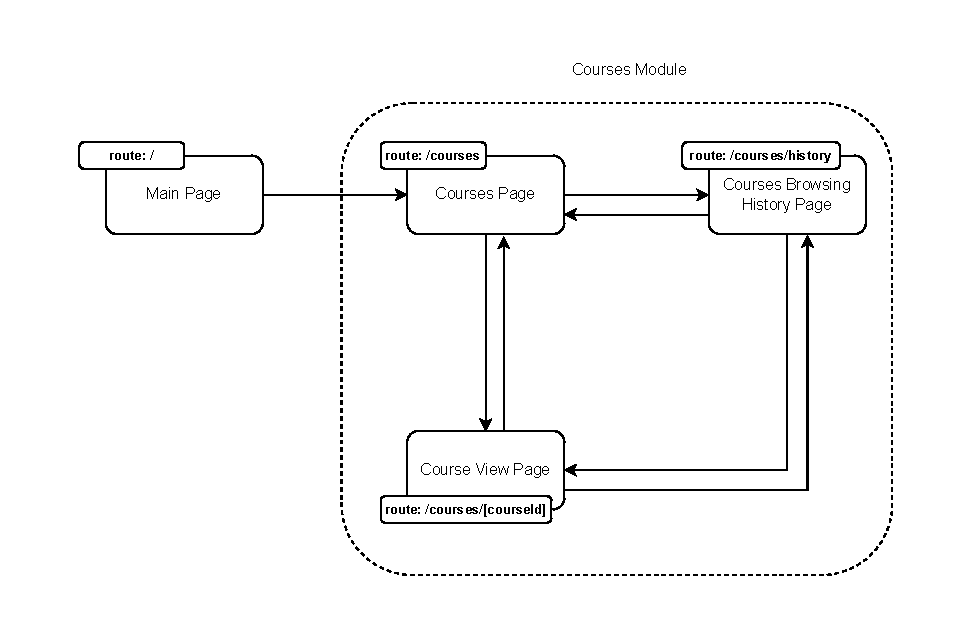
\includegraphics{images/course-reading-flow.pdf}
    \caption{User Flow - Reading courses}
    \label{fig:course-reading-flow}
\end{figure}

\newpage
\noindent Referring to the \textbf{main page} of the web platform as the starting point, the user can start reading courses by either clicking redirection links on the main page or by manually entering the course URLs. From Figure \ref{fig:course-reading-flow}, it can be observed that the user can navigate through the pages without being authenticated.
\\\\
\noindent The \textbf{courses page} is a list of all the courses available on the platform. From here, the user can click on a course from the list and be redirected to that course's view page. The route for the courses page can also receive the query parameter \textbf{search}, which will filter the courses based on the search query.
\\\\
\noindent The \textbf{courses browsing history page} is a list of all the courses that the user has visited. Selecting a course on this page will redirect to its view page.
\\\\
\noindent Both the courses page and the courses browsing history page are accessible through the global courses module navbar. Users can quickly navigate to these pages from any page that is part of the courses module.

\section{Manage courses}

\begin{figure}[h]
    \centering
    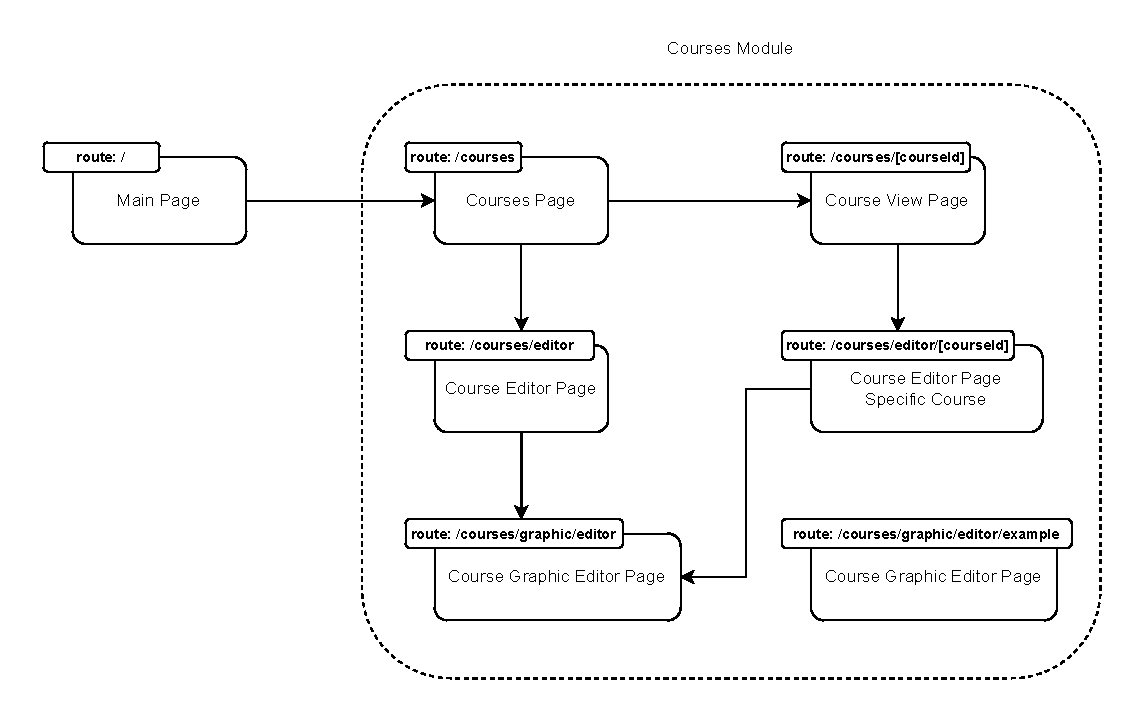
\includegraphics[scale=0.85]{images/course-manage-flow.pdf}
    \caption{User Flow - Manage courses}
    \label{fig:course-manage-flow}
\end{figure}

\newpage
\noindent All the editors are accessible even for unauthenticated users. The \textbf{course editor} is a page where a JSON editor is displayed, along with a live preview of how the editor's content will be rendered. It is accessible via the global courses module navbar. An unauthenticated user can play around in this editor and copy or download the JSON when they are satisfied with the result. In the case of authenticated users who also have the role of \textbf{Course Manager}, they can save the course to the database as a new course.
\\\\
\noindent The \textbf{course editor for a specific course} is the same as the course editor, but it is pre-filled with the content of the course given as a path variable. This editor is accessible from the course view page, by clicking the \textbf{Open in Editor} button. If the user is, once again, authenticated and has the role of \textbf{Course Manager}, they can save the course to the database as an update to the existing course. Unauthenticated users can still access a specific course editor, but they cannot save the course to the database. They are allowed because the official courses can be great examples of how to create their own courses.
\\\\
\noindent The graphic editor is a standalone editor that is accessible via the route mentioned in Figure \ref{fig:course-manage-flow} or via widgets from the course JSON editor. The difference between the two methods is that the first one opens an empty editor while the second method uses localStorage to pre-fill the graphic editor with one taken from the clicked widget. This page is the same for both authenticated and unauthenticated users, as the graphic needs to be copy-pasted into the course's content to be saved.
\\\\
\noindent The \textbf{course graphic editor page} from Figure \ref{fig:course-manage-flow} that is not connected to any other page can only be accessed via the route and contains a pre-filled example graphic that can still be edited.

\section{User authentication}

\noindent Authenticating the user is currently used only for allowing some people to manage the courses. The authentication flow is presented in Figure \ref{fig:user-auth-flow}.
\\\\
\noindent To start the authentication flow, you obviously need to do \textbf{step 1}, by entering the login page. The login page is accessible via the global navbar, by clicking the \textbf{Login} button. You can also manually navigate to the login page by entering the URL, but that would redirect to the main page.
\\\\
\noindent \textbf{Step 2} is to select the authentication provider. Currently, the only authentication providers usable are Discord and GitHub. Selecting a provider will trigger a redirection to one of \textbf{NextAuth's routes}, where the OAuth2 process will be started.
\\\\
\noindent \textbf{Step 3} is redirecting to the OAuth2 provider associated with the client registration selected. The user will be prompted to log in to the provider and authorize the web platform to access their account. After the user has authorized the web platform, they will be redirected back to the web platform in \textbf{step 4}.
\\\\
\noindent Based on the response from the OAuth2 provider, the NextAuth callback will decide if the user is authenticated or not. If an error has occurred, the user is redirected to the login page (taking the \textbf{5 error step}). If the user is authenticated with the OAuth2 server, the second part of the authentication process will be started. Following the \textbf{5 success step}, the Spring Boot authorization server will be called to generate a JWT token for the user. This token will be stored in the user's browser and will be used to authenticate the user in the future.
\\\\
\noindent The response, represented by \textbf{step 6}, will be processed by another NextAuth callback, which will either create a session for the user and redirect them to the page where the authentication flow started (\textbf{step 7 success}) or redirect them to the login page with an error message (\textbf{step 7 error}).
\\\\
\noindent Registration is not needed for the web platform, as the users are authenticated via OAuth2 providers. When authenticating the user, the backend auth server is responsible for managing the users and linking providers to the same account based on email.

\begin{figure}[h]
    \centering
    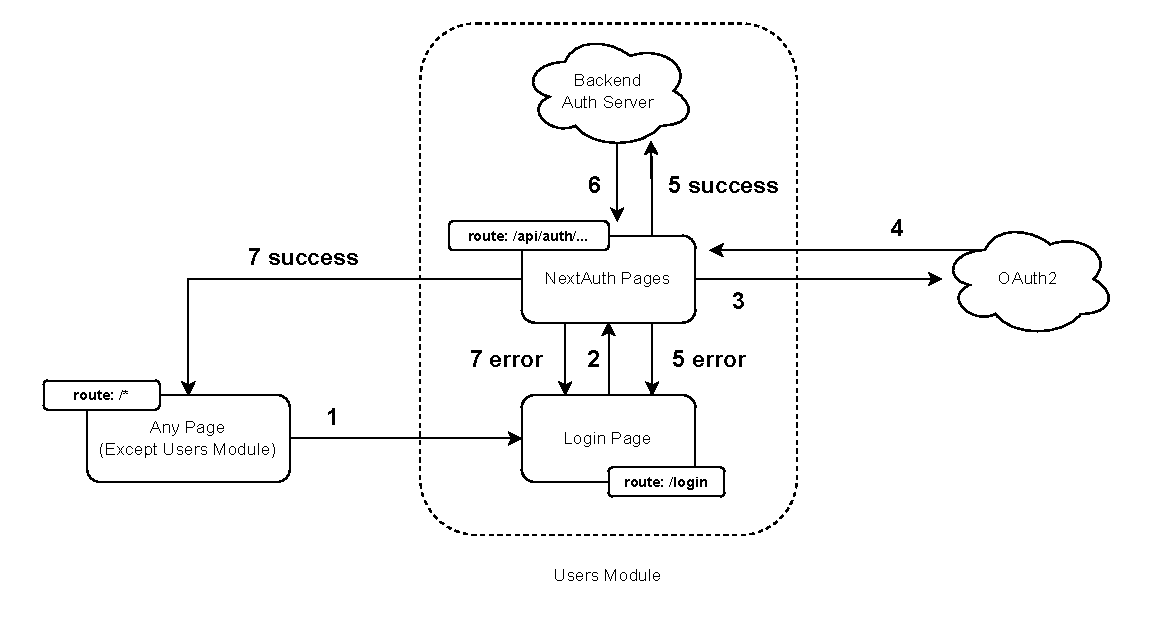
\includegraphics[scale=0.85]{images/user-auth-flow.pdf}
    \caption{User Flow - Authentication}
    \label{fig:user-auth-flow}
\end{figure}

\section{Accessing Resources}

\noindent After the user is authenticated, the session will contain two tokens generated by the authentication server. The first token is the access token, which is used to access protected resources. The second token is the refresh token, which is used to refresh the access token when it expires.
\\\\
\noindent Some resources are protected, while others are public but have protected actions. The public resources of the web platform are the courses, but editing them is a private action. The protected resources are the ones that require the user to be authenticated and have a specific role. The flow for accessing protected resources is presented in Figure \ref{fig:protected-resources-sequence}.

\begin{figure}[h]
    \centering
    \includegraphics{images/accessing-protected-resources-flow.pdf}
    \caption{Accessing protected resources sequence diagram}
    \label{fig:protected-resources-sequence}
\end{figure}

\noindent Requests from the frontend to access protected resources must be done with an access token, referred to in the Figure as a JWT. If no access token is specified in the request, the resource server will automatically reject the request with a 401 Unauthorized status code. That is only the case for resources that require authentication.
\\\\
\noindent The access token is validated in the second step, basically verifying that the token is properly formatted. This is done to prevent useless requests to the authorization server. If the token is not valid, the resource server will reject the request early with a 401 Unauthorized status code.
\\\\
\noindent To validate the token, the resource server will call the authorization server to check if the token is still valid. It will verify the signature of the token using the secret key of the authorization server. If the token is expired or has been tampered with, the resource server will reject the request with a 401 Unauthorized status code. The authorization server will also reject the token if it has been invalidated inside the database. If the token is valid, the resource server will continue processing the request.
\\\\
\noindent Now that the token is for sure valid, the resource server will check if the user has the required role to access the resource. If the user does not have the required role, the resource server will reject the request with a 403 Forbidden status code. If the user has the required role, the resource server will continue processing the request.
\\\\
\noindent The resource server will finally process the request and return the response to the frontend. The response will contain the requested data or an error message if something went wrong.
\\\\
\noindent The short dotted lines in the Figure represent an alternative flow, taken if the previous action was not already taken. For example, verifying if the token is valid is an alternative if the early reject action was not taken.
\\\\
\noindent Even if the Figure \ref{fig:protected-resources-sequence} presents the flow for accessing protected resources, the same flow applies to protected actions that do not necessarily involve returning data but are modifying it.
\chapter{Conclusions and Future Work}

\section{Conclusions}

In this thesis, I have documented the creation of a full-stack web application. The final product is a platform for visualizing design patterns through courses, which can be read and created within the application. The platform includes official courses and tools for creating more educational content. I've detailed the entire process, from choosing technologies to overcoming development challenges. This platform is useful for both students and teachers, offering a way to learn and teach design patterns. It separates course content from design, allowing course creators to focus on content while the platform handles the design. The source code is available on GitHub under the MIT license \cite{designoop}.
\\\\
\noindent Building a full stack application like this has been a goal of mine since I started programming. Creating a fully functional application from start to finish is a skill I believe I should have as a graduating computer science student. Through this project, I gained significant knowledge and experience, learning to use and integrate various technologies. I also focused on ensuring the application's security, performance, and ease of maintenance and extension.
\\\\
\noindent Although this was a complex and demanding project for one person, it lays the groundwork for an open-source community to contribute. This collaboration can improve the project, making it easier to maintain and manage with the shared expertise of experienced individuals.

\newpage
\section{Future Work}

The web platform leaves room for improvement and future work. If the project becomes popular within the open-source community, there will be many opportunities to improve the application. Here are some ideas for expanding the platform:

\begin{itemize}
\item \textbf{User Activity Tracking}: Currently, user accounts are only used for administrative purposes. This can be expanded to track user activity, such as course progress and completion.

\item \textbf{Course Recommendations}: The platform can be expanded to include course recommendations, allowing users to discover new courses based on their interests. This feature can be implemented using a recommendation engine that analyzes the previously mentioned user activity to recommend courses.

\item \textbf{Course Ratings and Reviews}: The platform can be expanded to include course ratings and reviews, allowing users to interact with the courses. Giving feedback can help improve the quality of the courses in the future.

\item \textbf{Quizzes}: Currently, the platform concentrates on design patterns courses, but it can be expanded to include quizzes as well. They would be a great addition to the platform and have a seamless integration with the courses. After a course or a group of courses is finished, the user can take a quiz to test their knowledge.

\item \textbf{Roadmaps}: When enough courses are established, branching in different directions and covering different topics, roadmaps can be created. These roadmaps can guide users through the courses, helping them understand the order in which they should take the courses.

\item \textbf{Community Forum}: Currently, the platform encourages user interaction externally, on either GitHub or Discord. A forum integrated within the platform could be a great addition. If a standalone forum is deemed unnecessary, the web platform could at least benefit from a section that unifies the discussions from external applications, such as a page that allows you to search through both GitHub issues and Discord topics at the same time.

\item \textbf{More Themes}: The application currently has a light and a dark theme. More themes can be added to the platform, allowing users to choose the one that suits them best. Besides the global themes for the application, course-specific themes may be added, providing themes that change only the course design while keeping the same content (e.g., a theme that makes the course more compact, one that adds more white space to it).

\item \textbf{Offline Mode}: The visited courses can be cached and made available offline. The course editor could be fully functional offline as well. Measures for this have already been taken, as the linting and suggestions are done on the client side.

\item \textbf{User Experience}: The user experience can be improved by adding more animations and transitions. The design of the courses themselves is also constantly evolving based on feedback received from users. The course and graphic editors can also be extended and modified to provide a better user experience for content creators. More intricate and specific features will be added to the editors as the platform grows and users request them.

\item \textbf{Design Patterns Editor}: Extending on the idea of helping users understand design patterns and interact with them more often, a special editor that highlights design patterns in the code can be developed. This editor could also offer suggestions on how to improve the code by applying design patterns. This idea can be implemented either as an editor inside the web platform or even as an extension to existing code editors.
\end{itemize}



\printbibliography[heading=bibintoc]

\end{document}